

\documentclass[letter,10pt,openany]{article}


\usepackage{amsmath,amsfonts,amssymb,amsthm}
\usepackage{color}
\usepackage{url}
\usepackage{fancyhdr}
\usepackage{alltt}
\usepackage{ifthen}
\usepackage{svn-multi}
\usepackage[latin1]{inputenc}
\usepackage{times}
\usepackage[T1]{fontenc}
\usepackage[pdftex]{graphicx}
\usepackage{array}
\usepackage[pdftex,colorlinks]{hyperref}
\graphicspath{{../figs/}{../Fig/}}  %% directories with  graphics files


\svnidlong          %experimenting with svn-multi
{$HeadURL: svn://zero.physics.gatech.edu/elton/blog/blog.tex $}
{$LastChangedDate: 2018-07-25 16:48:43 -0400 (Wed, 25 Jul 2018) $}
{$LastChangedRevision: 545 $}
{$LastChangedBy: predrag $}
\svnid{$Id: blog.tex 545 2018-07-25 20:48:43Z predrag $}
\svnkwsave{$RepoFile: elton/blog/blog.tex $}
\svnRegisterAuthor{jhalcrow}{Jonathan Halcrow}
\svnRegisterAuthor{elton}{John R. Elton}
\svnRegisterAuthor{predrag}{Predrag Cvitanovi{\'c}}
\svnRegisterAuthor{gibson}{John F. Gibson}
\svnRegisterAuthor{viswanath}{Divakar Viswanath}
\svnRegisterAuthor{afox33}{Adam Fox}
\svnRegisterAuthor{mfarazmand3}{Mohammad M. Farazmand}

%% If the svn information should be also placed
%% on the chapter page use:
%\fancypagestyle{plain}{%
%% otherwise use
\pagestyle{fancy}
\fancyhead{}
\fancyhead[er,ol]{\slshape \leftmark }
% \fancyfoot[er,ol]{rev. \svnrev\ (\svnfileauthor, rev. \svnfilerev )}
% \fancyfoot[el,or]{\svnfilemonth/\svnfileday/\svnfileyear}


% \input ../inputs/layout         %% page layout, ChaosBook environments
% editsDasbuch.tex
% $Author$ $Date$

% Predrag redefined \PC{...}							   15dec2010
% Predrag extracted from DasBuch def.tex                   25jun2008

\ifboyscout %%%%%%%% DISPLAY COMMENTS IN THE TEXT %%%%%%%%%%%%%%%%%%%%
            %%%%%%%% turn on labeling of equations on margins %%%%%%%%
    % also search the text for lines starting with %%  to
    % locate various internal comments, recent edits etc.
    \typeout{============ COMMENTED =====}
  \newcommand{\PublicPrivate}[2]
    {\marginpar{\color{blue}$\Downarrow$\footnotesize PRIVATE}%
    {\color{blue}#2}%
    \marginpar{\color{blue}$\Uparrow$\footnotesize PRIVATE}}
  \newcommand{\PC}[1]{$\footnotemark\footnotetext{Predrag: #1}$}
  % \newcommand{\PC}[1]{\\{\color{red} [{Predrag: #1}]}\\}
  \newcommand{\PCedit}[1]{{\color{magenta}#1}}
  \newcommand{\JG}[1]{$\footnotemark\footnotetext{John G: #1}$}
  \newcommand{\JGedit}[1]{{\color{magenta}#1}}
  \newcommand{\ES}[1]{$\footnotemark\footnotetext{Vaggelis: #1}$}
  \newcommand{\ESedit}[1]{{\color{red}#1}}
  \newcommand{\CS}[1]{$\footnotemark\footnotetext{Chao: #1}$}
  \newcommand{\CSedit}[1]{{\color{magenta}#1}}
  \newcommand{\AB}[1]{$\footnotemark\footnotetext{Annalisa: #1}$}
  \newcommand{\ABedit}[1]{{\color{red}#1}}
  \newcommand{\BB}[2]{$\footnotemark\footnotetext{Burak #1: #2}$}
  \newcommand{\BBedit}[1]{{\color{red}#1}}
  \newcommand{\RLD}[1]{$\footnotemark\footnotetext{Ruslan: #1}$}
  \newcommand{\RLDedit}[1]{{\color{magenta}#1}}
  \newcommand{\SF}[1]{$\footnotemark\footnotetext{Stefan: #1}$}
  \newcommand{\SFedit}[1]{{\color{magenta}#1}}
  \newcommand{\SOA}[1]{$\footnotemark\footnotetext{Sebastian: #1}$}
  \newcommand{\SOAedit}[1]{{\color{red}#1}}
  \newcommand{\DB}[2]{$\footnotemark\footnotetext{DB #1: #2}$} %date, comment
  \newcommand{\DBedit}[1]{{\color{green}#1}}
  \newcommand{\KC}[2]{$\footnotemark\footnotetext{KC #1: #2}$} %date, comment
  \newcommand{\KCedit}[1]{{\color{magenta}#1}}
  \newcommand{\Xiong}[2]{$\footnotemark\footnotetext{XD #1: #2}$} %date, comment
  \newcommand{\Xiongedit}[1]{{\color{green}#1}}
  \newcommand{\QG}[2]{$\footnotemark\footnotetext{QG #1: #2}$} %date, comment
  \newcommand{\QGedit}[1]{{\color{green}#1}}
  \newcommand{\MAP}[1]{$\footnotemark\footnotetext{Mason: #1}$}
  \newcommand{\LZ}[2]{$\footnotemark\footnotetext{LZ #1: #2}$} %date, comment
  \newcommand{\LZedit}[1]{{\color{green}#1}}
  \newcommand{\PMS}[2]{$\footnotemark\footnotetext{Pavel #1: #2}$} %date, comment
  \newcommand{\PMSedit}[1]{{\color{magenta}#1}}
  \newcommand{\TZ}[2]{$\footnotemark\footnotetext{Tingnan #1: #2}$} %date, comment
  \newcommand{\TZedit}[1]{{\color{green}#1}}
  \newcommand{\BM}[2]{$\footnotemark\footnotetext{Ben #1: #2}$} %date, comment
  \newcommand{\BMedit}[1]{{\color{green}#1}}
  \newcommand{\GX}[2]{$\footnotemark\footnotetext{Guopeng #1: #2}$} %date, comment
  \newcommand{\GXedit}[1]{{\color{green}#1}}
  \newcommand{\JPE}[2]{$\footnotemark\footnotetext{James #1: #2}$} %date, comment
  \newcommand{\JPEedit}[1]{{\color{red}#1}}
  \newcommand{\Private}[1]{{\color{blue}#1}}
    %    \newcommand{\Preliminary}[1]
    %{\marginpar{\color{magenta}$\Downarrow$\footnotesize PRELIMINARY}%
    %{\color{magenta}#1}%
    %\marginpar{\color{magenta}$\Uparrow$\footnotesize PRELIMINARY}}
\else % drop comments
      % do not turn on labeling of equations on margins
  \typeout{============ UNCOMMENTED =====}
  \newcommand{\PublicPrivate}[2]{#1}
  \newcommand{\PC}[1]{}
  \newcommand{\PCedit}[1]{#1}
  \newcommand{\JG}[1]{}
  \newcommand{\JGedit}[1]{#1}
  \newcommand{\ES}[1]{}
  \newcommand{\ESedit}[1]{#1}
  \newcommand{\CS}[1]{}
  \newcommand{\CSedit}[1]{#1}
  \newcommand{\AB}[1]{}
  \newcommand{\ABedit}[1]{#1}
  \newcommand{\BB}[2]{}{}
  \newcommand{\BBedit}[1]{#1}
  \newcommand{\RLD}[1]{}
  \newcommand{\RLDedit}[1]{#1}
  \newcommand{\SF}[1]{}
  \newcommand{\SFedit}[1]{#1}
  \newcommand{\SOA}[1]{}
  \newcommand{\SOAedit}[1]{#1}
  \newcommand{\DB}[2]{}{}
  \newcommand{\DBedit}[1]{#1}
  \newcommand{\KC}[2]{}{}
  \newcommand{\KCedit}[1]{#1}
  \newcommand{\Xiong}[2]{}{} %date, comment
  \newcommand{\Xiongedit}[1]{#1}
  \newcommand{\QG}[2]{}{} %date, comment
  \newcommand{\QGedit}[1]{#1}
  \newcommand{\MAP}[1]{}
  \newcommand{\LZedit}[1]{#1}
  \newcommand{\PMS}[2]{}
  \newcommand{\PMSedit}[1]{#1}
  \newcommand{\TZ}[2]{}
  \newcommand{\TZedit}[1]{#1}
  \newcommand{\BM}[2]{}
  \newcommand{\BMedit}[1]{#1}
  \newcommand{\Private}[1]{}
\fi  %%%%%%%%%%%% END OF ON/OFF COMMENTS SWITCH %%%%%%%%%%%%%%%%%%%%
  %% editing comments, DasBuch style
% def.tex
% $Author$ $Date$

%%%%%%%%%%%%%%%%%%%%%%%%%%%%%%%%%%%%%%%%%%%%%%%%%%%%%%%%%%%%%%%%%%%%%%%%%
%% defines macros used throughout ChaosBook and related
%%%%%%%%%%%%%%%%%%%%%%%%%%%%%%%%%%%%%%%%%%%%%%%%%%%%%%%%%%%%%%%%%%%%%%%%%

%               Predrag         27feb2012
%               Predrag         17feb2012
%               Predrag          4feb2012
%               Predrag          9oct2009
%               Predrag         12jun2008
%               Predrag         15dec2008
%               Predrag         29oct2005
%               Predrag         13jul2005
%               Predrag         24apr2005
%               Predrag         14feb2005
%               Predrag         22jan2005
%               Predrag         16nov2004
%               Predrag         13jun2004
%               Predrag          3may2004
%               Predrag         10apr2004
%               Predrag         21feb2004
%               Predrag          4oct2003
%               Predrag         30aug2003
%               Predrag         20jun2003
%               Predrag         17jan2003
%               Predrag          6dec2002
%               Predrag          7jul2002
%               Predrag         19nov2000
%               Ronnie          23sep2000
% Predrag disabled \basedirectory machine identifier    25aug2000
% Predrag created               30oct1994

\ifpaper % prepare for B&W paper printing:
       \newcommand{\href}[2]{{#2}}  % no hyperref
       \newcommand{\HREF}[2]{{#2}}
       \renewcommand{\color}[1]{}       % B&W
       \newcommand{\wwwcb}[1]{{ChaosBook.org#1}}
       \newcommand{\wwwgt}{{birtracks.eu}}
       \newcommand{\wwwQFT}[1]{{ChaosBook.org/\-Field\-Theory#1}}
       \newcommand{\wwwcnsQFT}[1]{{ChaosBook.org/\-Field\-Theory#1}}
       \newcommand{\weblink}[1]{{#1}}
       \newcommand{\arXiv}[1]{ {arXiv:#1}}
       \newcommand{\mpArc}[1]{{mp\_arc~#1}}
\else % prepare hyperlinked pdf
        \newcommand{\wwwcb}[1]{       % keep homepage flexible:
                  {\href{http://ChaosBook.org#1}
              {ChaosBook.org#1}}}
       \newcommand{\wwwgt}{{\href{http://birtracks.eu}
              {birtracks.eu}}}
       \newcommand{\wwwQFT}[1]{
                  {\href{http://ChaosBook.org/FieldTheory#1}
              {ChaosBook.org/\-Field\-Theory#1}}}
       \newcommand{\wwwcnsQFT}[1]{
                  {\href{http://ChaosBook.org/FieldTheory#1}
              {ChaosBook.org/\-Field\-Theory#1}}}
       \newcommand{\weblink}[1]{{\href{http://#1}{#1}}}
       \newcommand{\HREF}[2]{
              {\href{#1}{#2}}}
       \newcommand{\mpArc}[1]{
              {\href{http://www.ma.utexas.edu/mp_arc-bin/mpa?yn=#1}
                   {mp\_arc~#1}}}
       \newcommand{\arXiv}[1]{
              {\href{http://arXiv.org/abs/#1}{arXiv:#1}}}
\fi

%%%%%%%%%%%%%%%%%%%%%% QUOTATIONS %%%%%%%%%%%%%%%%%%%%%%%%%%%%%%%%%%%%%%
%
%  the learned/witty quotes at the chapter and section headings
%
\newsavebox{\bartName}
\newcommand{\bauthor}[1]{\sbox{\bartName}{\parbox{\textwidth}{\vspace*{0.8ex}
       %\hspace*{\fill}
       \hspace{2em}---\small\noindent #1}}}
\newenvironment{bartlett}{\hfill\begin{minipage}[t]{0.65\textwidth}\small}%
{\hspace*{\fill}\nolinebreak[1]\usebox{\bartName}\vspace*{1ex}\end{minipage}}
%
%  a quotation inserted into the text
%
\newenvironment{txtquote}{\begin{quotation} \small}{\end{quotation}}

\newcommand{\student}{Henriette Roux}
%\newcommand{\student}{Jens J. Jensen}

%%%%%%%%%%%%%%%%%%%%%% INDEXING %%%%%%%%%%%%%%%%%%%%%%%%%%%%%%%%%%%%%%%%%
\newcommand{\indx}[1] {#1\index{#1}}    % do not need to repeat the word

\newcommand{\file}[1]{$\footnotemark\footnotetext{{\bf file} #1}$}
% PC 9sep2008 commented out (is it used?):
%\newcommand{\lecture}[2]{ \addtocontents{toc}
%           {{\scriptsize #1}{\sf\small lecture: \scriptsize #2}} }

%%%%%%%%%%%%%%% EQUATIONS %%%%%%%%%%%%%%%%%%%%%%%%%%%%%%%
\newcommand{\beq}{\begin{equation}}
\newcommand{\continue}{\nonumber \\ }
\newcommand{\nnu}{\nonumber}
\newcommand{\eeq}{\end{equation}}
\newcommand{\ee}[1] {\label{#1} \end{equation}}
\newcommand{\bea}{\begin{eqnarray}}
\newcommand{\ceq}{\nonumber \\ & & }
\newcommand{\eea}{\end{eqnarray}}
\newcommand{\barr}{\begin{array}}
\newcommand{\earr}{\end{array}}

%%%%%%%%%%%%%%% REFERENCING EQUATIONS ETC. %%%%%%%%%%%%%%%%%%%%%%%%%%%%%%%
\newcommand{\rf}     [1] {~\cite{#1}}
\newcommand{\refref} [1] {ref.~\cite{#1}}
\newcommand{\refRef} [1] {Ref.~\cite{#1}}
\newcommand{\refrefs}[1] {refs.~\cite{#1}}
\newcommand{\refRefs}[1] {Refs.~\cite{#1}}
\newcommand{\refeq}  [1] {(\ref{#1})}
\newcommand{\refeqs} [2]{(\ref{#1}--\ref{#2})}
\newcommand{\refpage}[1] {page~\pageref{#1}}
\newcommand{\reffig} [1] {figure~\ref{#1}}
\newcommand{\reffigs} [2] {figures~\ref{#1} and~\ref{#2}}
\newcommand{\refFig} [1] {Figure~\ref{#1}}
\newcommand{\refFigs} [2] {Figures~\ref{#1} and~\ref{#2}}
\newcommand{\reftab} [1] {table~\ref{#1}}
\newcommand{\refTab} [1] {Table~\ref{#1}}
\newcommand{\reftabs}[2] {tables~\ref{#1} and~\ref{#2}}
\newcommand{\refsect}[1] {sect.~\ref{#1}}
\newcommand{\refsects}[2] {sects.~\ref{#1} and \ref{#2}}
\newcommand{\refSect}[1] {Sect.~\ref{#1}}
\newcommand{\refSects}[2] {Sects.~\ref{#1} and \ref{#2}}
\newcommand{\refsecttosect}[2] {Sects.~\ref{#1} to~\ref{#2}}
\newcommand{\refchap}[1] {chapter~\ref{#1}}
\newcommand{\refChap}[1] {Chapter~\ref{#1}}
\newcommand{\refchaps}[2] {chapters~\ref{#1} and~\ref{#2}}
\newcommand{\refchaptochap}[2] {chapters~\ref{#1} to~\ref{#2}}
\newcommand{\refappe}[1] {appendix~\ref{#1}}
\newcommand{\refappes}[2] {appendices~\ref{#1} and~\ref{#2}}
\newcommand{\refAppe}[1] {Appendix~\ref{#1}}
\newcommand{\refrem} [1] {remark~\ref{#1}}
\newcommand{\refexam}[1] {example~\ref{#1}}
\newcommand{\refExam}[1] {Example~\ref{#1}}
\newcommand{\refexer}[1] {exercise~\ref{#1}}
\newcommand{\refExer}[1] {Exercise~\ref{#1}}
\newcommand{\refsolu}[1] {solution~\ref{#1}}
\newcommand{\refSolu}[1] {Solution~\ref{#1}}

%%%%%%%%%%%%%%  Abbreviations %%%%%%%%%%%%%%%%%%%%%%%%%%%%%%%%%%%%%%%%
%%% APS (American Physiology Society, it seems) style:
%%%     Latin or foreign words or phrases should be roman, not italic.
%%%     Insert a `hard' space after full points
%%%                                         that do not end sentences.

\newcommand{\etc}{{etc.}}       % APS
\newcommand{\etal}{{\em et al.}}    % etal in italics, APS too
\newcommand{\ie}{{i.e.}}        % APS
\newcommand{\cf}{{\em cf.\ }}     % APS
\newcommand{\eg}{{e.g.\ }}        % APS, OUP, hard space '\eg\ NextWord'
% \newcommand{\etc}{{\em etc.}}     % etcetera in italics
% \newcommand{\ie}{{that is}}       % use Latin or English?  Decide later.
% \newcommand{\cf}{{cf.}}
% \newcommand{\eg}{{\it e.g.,\ }}   % Wirzba 2sep2001

%%%%%%%%%%%%%%% ChaosBook Abbreviations %%%%%%%%%%%%%%%%%%%%%%%%

\newcommand{\evOper}{evolution oper\-ator}
\newcommand{\EvOper}{Evolution oper\-ator}
 %% \newcommand{\evOp}{Ruelle operator} %could be ``evolution'' instead?
%\newcommand{\FPoper}{Frobenius-Perron oper\-ator}
\newcommand{\FPoper}{Perron-Frobenius oper\-ator} % Pesin's ordering
\newcommand{\FP}{Perron-Frobenius}
\newcommand{\statesp}{state space}
\newcommand{\Statesp}{State space}
\newcommand{\fixedpnt}{fixed point}
\newcommand{\Fixedpnt}{fixed point}
\newcommand{\maslov}{topological}
\newcommand{\Maslov}{Topological}
%\newcommand{\Maslov}{Keller-Maslov}
\newcommand{\jacobian}{Jacobian}        % determinant
% \newcommand{\jacobianM}{fundamental matrix} % no known standard name?
% \newcommand{\jacobianMs}{fundamental matrices}  %
% \newcommand{\JacobianM}{Fundamental matrix} %
% \newcommand{\JacobianMs}{Fundamental matrices}  %
\newcommand{\jacobianM}{Jacobian matrix}  % back to Predrag's name 20oct2009
\newcommand{\jacobianMs}{Jacobian matrices}   % matrices
\newcommand{\JacobianM}{Jacobian matrix} %
\newcommand{\JacobianMs}{Jacobian matrices}  %
\newcommand{\FloquetM}{Floquet matrix} % specialized to periodic orb
\newcommand{\FloquetMs}{Floquet matrices}  %
% \newcommand{\stabmat}{matrix of variations}   % Arnold, says Vattay
\newcommand{\stabmat}{stability matrix}     % stability matrix, velocity gradients
\newcommand{\Stabmat}{Stability matrix}     % Stability matrix
\newcommand{\stabmats}{stability matrices}
\newcommand{\monodromyM}{monodromy matrix} % monodromy matrix, Poincare cut
\newcommand{\MonodromyM}{Monodromy matrix} % monodromy matrix, Poincare cut
\newcommand{\dzeta}{dyn\-am\-ic\-al zeta func\-tion}
\newcommand{\Dzeta}{Dyn\-am\-ic\-al zeta func\-tion}
\newcommand{\tzeta}{top\-o\-lo\-gi\-cal zeta func\-tion}
\newcommand{\Tzeta}{Top\-o\-lo\-gi\-cal zeta func\-tion}
\newcommand{\BERzeta}{BER zeta func\-tion}
%\newcommand{\tzeta}{Artin-Mazur zeta func\-tion} %alternative to topological
\newcommand{\qS}{semi\-classical zeta func\-tion}
%\newcommand{\qS}{Gutz\-willer-Voros zeta func\-tion}
\newcommand{\Gt}{Gutz\-willer trace formula}
\newcommand{\Fd}{spec\-tral det\-er\-min\-ant}
%\newcommand{\fd}{spec\-tral det\-er\-min\-ant} %in many articles
\newcommand{\FD}{Spec\-tral det\-er\-min\-ant}
\newcommand{\cFd}{semiclass\-ic\-al spec\-tral det\-er\-mi\-nant}
\newcommand{\cFD}{Semiclass\-ic\-al spec\-tral det\-er\-mi\-nant}
% \newcommand{\cFd}{semiclass\-ic\-al Fred\-holm det\-er\-mi\-nant}
\newcommand{\Vd}{Vattay det\-er\-mi\-nant}
\newcommand{\cycForm}{cycle averaging formula}
\newcommand{\CycForm}{Cycle averaging formula}
\newcommand{\freeFlight}{mean free flight time}
\newcommand{\FreeFlight}{Mean free flight time}
\newcommand{\pdes}{partial differential equations}
\newcommand{\Pdes}{Partial differential equations}
\newcommand{\dof}{dof}         % Hamiltonian deegree of freedom
% \newcommand{\dof}{deegree of freedom}

%%%%%%%%%%%%%%% VECTORS, MATRICES, NORMS %%%%%%%%%%%%%%%%%%%%%%%%%%%%%%%%%

	% without large brackets:
\newcommand{\braket}[2]
		   {\langle{#1}\vphantom{#2}|\vphantom{#1}{#2}\rangle}
\newcommand{\bra}[1]{\langle{#1}\vphantom{ }|}
\newcommand{\ket}[1]{|\vphantom{}{#1}\rangle}
	% with large brackets:
%\newcommand{\bra}[1]{\left\langle{#1}\vphantom{ }\right|}
%\newcommand{\ket}[1]{\left|\vphantom{}{#1}\right\rangle}
%\newcommand{\braket}[2]{\left\langle{#1}
%                        \vphantom{#2}\right|\left.\vphantom{#1}
%                        {#2}\right\rangle}

\newcommand{\dual}[1]{{#1}^\ast}
% \newcommand{\transp}[1]{\bar{#1}}
\newcommand{\transp}[1]{{#1}{}^\top}

% Commented out AMS-style pmatrix, which is incompatible with TeX/LaTeX pmatrix
% used throughout dasbuch. Fri Oct 12 15:51:03 EDT 2007

\newcommand{\MatrixII}[4]{\left(
\begin{array}{cc}
{#1}  &  {#2} \\
{#3}  &  {#4} \end{array} \right)}
% a problem with \pmatrix 12oct 2007
%\newcommand{\MatrixII}[4]{
%   \begin{pmatrix}{#1}  &  {#2} \\
%                  {#3}  &  {#4} \end{pmatrix}}

\newcommand{\MatrixIII}[9]{
  \pmatrix{ {#1}  &  {#2} &  {#3} \cr
            {#4}  &  {#5} &  {#6} \cr
            {#7}  &  {#8} &  {#9}
          }               }
% \newcommand{\MatrixIII}[9]{
%    \begin{pmatrix} {#1}  &  {#2} &  {#3} \\
%                    {#4}  &  {#5} &  {#6} \\
%                    {#7}  &  {#8} &  {#9}  \end{pmatrix}}


% \newcommand{\transpVectorII}[2]{
%    \begin{pmatrix}{#1}  &  {#2}  \end{pmatrix}}

\newcommand{\VectorII}[2]{\left(
\begin{array}{cc}
{#1}  &  {#2} \end{array} \right)}
%
%\newcommand{\VectorII}[2]{
%  \pmatrix{ {#1} \cr {#2}}
%}

% \newcommand{\VectorII}[2]{
%    \begin{pmatrix} {#1} \\
%                    {#2}  \end{pmatrix}}

% \newcommand{\VectorIII}[3]{
%    \begin{pmatrix} {#1} \\
%                    {#2} \\
%                    {#3} \end{pmatrix}}

\newcommand{\transpVectorII}[2]{
  \pmatrix{ {#1}  &  {#2}}
}

\newcommand{\VectorIII}[3]{
  \pmatrix{ {#1} \cr
            {#2} \cr
            {#3}
          }
}

\newcommand{\combinatorial}[2]{ {#1 \choose #2}}

%%%%%%%%%%%%%%% Sundry symbols within math eviron.: %%%%%%%%%%%%

\newcommand{\obser}{\ensuremath{a}}     % an observable from phase space to R^n
\newcommand{\Obser}{\ensuremath{A}}     % time integral of an observable
\newcommand{\onefun}{\iota} % the function that returns one no matter what
\newcommand{\defeq}{=}      % the different equal for a definition
\newcommand {\deff}{\stackrel{\rm def}{=}}
\newcommand{\reals}{\mathbb{R}}
\newcommand{\complex}{\mathbb{C}}
\newcommand{\integers}{\mathbb{Z}}
\newcommand{\rationals}{\mathbb{Q}}
\newcommand{\naturals}{\mathbb{N}}
\newcommand{\LieD}{{{\cal L}\!\!\llap{-}\,\,}}  % {{\pound}} % Lie Derivative
\newcommand{\half}{{\scriptstyle{\frac{1}{2}}}}
\newcommand{\pde}{\partial}
\newcommand{\pdfrac}[2]{\frac{\partial #1}{\partial #2}}
\renewcommand\Im{\ensuremath{{\rm Im}\,}}
\renewcommand\Re{\ensuremath{{\rm Re}\,}}
\renewcommand{\det}{\mbox{\rm det}\,}
\newcommand{\Det}{\mbox{\rm Det}\,}
\newcommand{\tr}{\mbox{\rm tr}\,}
\newcommand{\Tr}{\mbox{\rm tr}\,}
%\newcommand{\Tr}{\mbox{Tr}\,}
\newcommand{\sign}[1]{\sigma_{#1}}
%\newcommand{\sign}[1]{{\rm sign}(#1)}
\newcommand{\mInv}{{I}}                 % material invariant
\newcommand{\msr}{\ensuremath{\rho}}                % measure
\newcommand{\Msr}{{\mu}}                % coarse measure
\newcommand{\dMsr}{{d\mu}}              % measure infinitesimal
\newcommand{\SRB}{{\rho_0}}             % natural measure
\newcommand{\vol}{{V}}                  % volume of i-th tile
\newcommand{\prpgtr}[1]{\delta\negthinspace\left( {#1} \right)}
%\newcommand{\Zqm}{\ensuremath{Z_{qm}}}         % Gutz-Voros zeta function
\newcommand{\Zqm}{\ensuremath{\det(\hat{H} - E)_{sc} }} % semicls spectr. det:
\newcommand{\Fqm}{\ensuremath{F_{qm}}}
\newcommand{\zfct}[1]{\zeta ^{-1}_{#1}}
\newcommand{\zetaInv}{\ensuremath{1/\zeta}}
% \newcommand{\zetaInv}{{\zeta^{-1}}}
\newcommand{\zetatop}{\ensuremath{1/\zeta_{\mbox{\footnotesize top}} }}
\newcommand{\zetaInvBER}[1]{1/\zeta_{\mbox{\footnotesize BER}}(#1)}
\newcommand{\BER}[1]{{\mbox{\footnotesize BER}}} % Baladi-Ruelle-Eckmann
\newcommand{\eigCond}{\ensuremath{F}}           % eigenvalue cond. function
\newcommand{\expct}    [1]{\left\langle {#1} \right\rangle}
\newcommand{\spaceAver}[1]{\left\langle {#1} \right\rangle}
\newcommand{\timeAver} [1]{\overline{#1}}
\newcommand{\norm}[1]{\left\Arrowvert \, #1 \, \right\Arrowvert}
\newcommand{\pS}{\ensuremath{{\cal M}}}          % symbol for state space
\newcommand{\ssp}{\ensuremath{x}}                % state space point
\newcommand{\tissp}{\tilde{\Delta\ssp}} % Rytis \CostFct
\newcommand{\pSpace}{x}       % Hamiltonian phase space x=(q,p) coordinate
\newcommand{\coord}{q}        % configuration space p coordinate
\newcommand{\DOF}{\ensuremath{D}}          % Hamiltonian deegree of freedom
\newcommand{\NWS}{\ensuremath{\Omega}}     % symbol for the non--wandering set
\newcommand{\AdmItnr}{\Sigma}      % set of admissible itineraries
\newcommand{\intM}[1]{{\int_\pS{\!d #1}\:}} %phase space integral
\newcommand{\Cint}[1]{\oint\frac{d#1}{2 \pi i}\;} %Cauchy contour integral
\newcommand{\PoincS}{\ensuremath{{\cal P}}}  % symbol for Poincare section
\newcommand{\PoincM}{\ensuremath{P}}       % symbol for Poincare map
\newcommand{\PoincC}{\ensuremath{U}}       % symbol for Poincare constraint function
\newcommand{\arc}{\ensuremath{s}}          % symbol for billiard wall arc
\newcommand{\mompar}{\ensuremath{p}}       % billiard wall parall. momentum
\newcommand{\restCoeff}{\ensuremath{\gamma}}  % billiard wall restitution coeff
\newcommand{\timeIn}[1]{{t^{-}_{#1}}} % billiard wall time of arrival
\newcommand{\timeOut}[1]{{t^{+}_{#1}}}   % billiard wall time of departure
%\newcommand{\PoincS}{\partial{\cal M}}          % billiard Poincare section
\newcommand{\Lop}{\ensuremath{{\cal L}}}       % evolution operator
\newcommand{\Uop}{\ensuremath{{\cal K}}}       % Koopman operator, Driebe notation
%\newcommand{\Uop}{\ensuremath{{\cal L}^\dagger}}  % Koopman, adjoint notation
\newcommand{\Aop}{\ensuremath{{\cal A}}}       % evolution generator
\newcommand{\TrOp}{\ensuremath{{\cal T}}}       % transfer operator, like in statmech
\newcommand{\matId}{\ensuremath{{\bf 1}}}      % matrix identity
\newcommand{\eigenvL}{\ensuremath{s}}      % evolution operator eigenvalue
\newcommand{\eigenvG}{\ensuremath{m}}      % compact group eigenvalues
\newcommand{\inFix}[1]{{\in \mbox{\footnotesize Fix}f^{#1}}}
\newcommand{\inZero}[1]{{\in \mbox{\footnotesize Zero} \, f^{#1} }}
\newcommand{\xzero}[1]{{x_{#1}^\ast}}
\newcommand{\fractal}{{{\cal F}}}
\newcommand{\contract}{F}
% \newcommand{\presentation}{P} % PC commented out 7sep2008
\newcommand{\orderof}[1]{o(#1)} % Rytis 22mar2005

     %%%%%%%%%% flows: %%%%%%%%%%%%%%%%%%%%%%%%%%%%
\newcommand\map{f}                  % other people like \phi's etc
\newcommand\flow[2]{{f^{#1}(#2)}}
\newcommand{\vel}{\ensuremath{v}}   % state space velocity
\newcommand\velField[1]{{v(#1)}}    % ODE velocity field
\newcommand\invFlow{F}
\newcommand\hflow[2]{{\hat{f}^{#1}(#2)}}
\newcommand\timeflow{{f^t}}
\newcommand\tflow[2]{{\tilde{f}^{#1}(#2)}}
%\newcommand\tflow{\tilde{f}^\tau}        %RECHECK USE OF THIS!
\newcommand\xInit{{x_0}}        %initial x
%\newcommand\xInit{\xi}     %initial x, Spiegel notation
\newcommand{\para}{\parallel}
\newcommand\multiX{x}       %multi point n-dim vector
\newcommand\multiF{f}       %multi point n-dim vector mapping

   %%%%%%% 3D physical flow
\newcommand{\stagp}{stagnation point}
\newcommand{\Stagp}{Stagnation point}
\newcommand{\relstagp}{traveling stagnation point}
\newcommand{\Relstagp}{Traveling stagnation point}
\newcommand{\velgradmat}{velocity gradients matrix}

   %%%%%%%% Siminos thesis %%%%%%%%%%%%%%%%%%%%%%%%%%%%
\newcommand{\Le}{Lorenz equations}
\newcommand{\rLor}{\rho}    % parameter r in Lorenz paper
\newcommand{\cLe}{complex Lorenz equations}
\newcommand{\cLf}{complex Lorenz flow}
\newcommand{\CLe}{Complex Lorenz equations}
\newcommand{\CLf}{Complex Lorenz flow}
\newcommand{\RerCLor}{\rho_1}    % real      part of parameter r, CLe
\newcommand{\ImrCLor}{\rho_2}    % imaginary part of parameter r, CLe
% \newcommand{\AGHe}{Armbruster-Guckenheimer-Holmes flow}

     %%%%%%%%%% periods: %%%%%%%%%%%%%%%%%%%%%%%%%%%%
\newcommand\period[1]{{\ensuremath{T_{#1}}}}         %continuous cycle period
%\newcommand\period[1]{{\tau_{#1}}}
\newcommand{\cl}[1]{{\ensuremath{n_{#1}}}}   % discrete length of a cycle, Predrag
%\newcommand{\cl}[1]{|#1|}  % the length of a periodic orbit, Ronnie
\newcommand{\nCutoff}{N}    % maximal cycle length
                % maximal stability cutoff:
\newcommand{\stabCutoff}{\ExpaEig_{\mbox{\footnotesize max}}}
\newcommand{\timeSegm}[1]{{\tau_{#1}}}      %billiard segment time period
\newcommand{\timeStep}{\ensuremath{{\delta \tau}}}  %integration step
\newcommand{\deltaX}{\ensuremath{{\delta x}}}       %trajectory displacement
\newcommand{\unitVec}{\ensuremath{\hat{n}}}     %unit vector

\newcommand{\Mvar}{\ensuremath{A}}  % stability matrix
\newcommand{\derF}[1]{\ensuremath{A(#1)}}   % Predrag stability matrix
 %\newcommand{\derF}[1]{{DF |_{#1}}}        % Gibson stability matrix
\newcommand{\jMps}{\ensuremath{J}}   % jacobian matrix, phase space/state space
% \newcommand{\jMps}{\ensuremath{{\bf J}}}  % bold fundamental matrix phase space
\newcommand{\derf}[2]{\ensuremath{{J}^{#1}(#2)}}    % Predrag fundamental matrix
% \newcommand{\derf}[2]{\ensuremath{{\bf J}^{#1}(#2)}}  % Predrag bold fundamental matrix
 % \newcommand{\derf}[2]{{Df^{#1}|_{#2}}}   % Gibson fundamental matrix
\newcommand{\jMConfig}{\ensuremath{{\bf j}}}    % fundamental matrix, configuration space
\newcommand{\jConfig}{\ensuremath{j}}      % jacobian, configuration space
\newcommand{\jMP}{\ensuremath{\hat{J}}}   % jacobian matrix, Poincare return
% \newcommand{\jMP}{\ensuremath{{\bf \hat{J}}}}   % bold jacobian matrix, Poincare return
\newcommand{\monodromy}{\ensuremath{M}}   % monodromy matrix, full Poincare cut
% \newcommand{\monodromy}{\ensuremath{{\bf M}}}   % bold monodromy matrix, full Poincare cut
                   % Fredholm det jacobian weight:
%\newcommand{\jEigvec}[1]{\ensuremath{{\bf e}^{(#1)}}}  % right jacobiam eigenvector
%\newcommand{\jEigvecT}[1]{\ensuremath{{\bf e}_{(#1)}}}  % left jacobiam eigenvector
\newcommand{\jEigvec}[1][]{\ensuremath{{\bf e}^{(#1)}}} % right jacobiam eigenvector
\newcommand{\jEigvecT}[1][]{\ensuremath{{\bf e}_{(#1)}}} % left jacobiam eigenvector
\newcommand{\oneMinJ}[1]
           {\left|\det\!\left(\matId-\monodromy_p^{#1}\right)\right|}
\newcommand{\maslovInd}{\ensuremath{m}}        % Maslov index
\newcommand{\ExpaEig}{\ensuremath{\Lambda}}
\newcommand{\Lyap}{\ensuremath{\lambda}}            %Lyapunov exponent

%%   optional parameter comes in [\ldots], for example
%%   \newcommand\eigRe[1][ ]{\ensuremath{\mu_{#1}}}
%%   no subscript: \eigRe\
%%   with subscript j: \eigRe[j]
%%
% \newcommand{\eigExp}[1][ ]{\ensuremath{\lambda_{#1}}}   % complex eigenexponent
%%  Guckenheimer&Holmes:  lambda = alpha + i beta
%%  Hirsch-Smale:         lambda = a     + i b
%%  Boyce-di Prima:       lambda = mu    + i nu
% \newcommand{\eigRe}[1][ ]{\ensuremath{\mu_{#1}}}    % Re eigenexponent
% \newcommand{\eigIm}[1][ ]{\ensuremath{\nu_{#1}}}    % Im eigenexponent

\newcommand{\eigExp}[1][]{
     \ifthenelse{\equal{#1}{}}{\ensuremath{\lambda}}{\ensuremath{\lambda^{(#1)}}}}
\newcommand{\eigRe}[1][]{
     \ifthenelse{\equal{#1}{}}{\ensuremath{\mu}}{\ensuremath{\mu^{(#1)}}}}
\newcommand{\eigIm}[1][]{
     \ifthenelse{\equal{#1}{}}{\ensuremath{\omega}}{\ensuremath{\omega^{(#1)}}}}

\newcommand\LyapTime{T_{\mbox{\footnotesize Lyap}}} %Lyapunov time
\newcommand{\hatx}{{\hat{x}}}
% \newcommand{\hatx}{{\hat{x}_t}}               %RECHECK USE OF THIS!
\newcommand{\hatp}{{\hat{x}_p}}
\newcommand{\phat}{{\hat{p}}}
\newcommand{\curvR}{\rho}           %billiard curvature
\newcommand{\dz}{{\delta z}}
\newcommand{\dth}{{\delta \theta}}
\newcommand{\delh}{{\delta h}}
\newcommand{\NN}{{{\cal N}}}

%%%%%%%%%%%%%%% symbolic dynamics %%%%%%%%%%%%%%%%%%%%%%%%%%%%%%%%%%
\newcommand{\MarkGraph}{Transition graph} % following Yorke
\newcommand{\markGraph}{transition graph} % following Yorke
% \newcommand{\MarkGraph}{Markov graph}
\newcommand{\admissible}{admissible}
\newcommand{\Admissible}{Admissible}
\newcommand{\inadmissible}{inadmissible}
\newcommand{\cycle}[1]{{\ensuremath{\overline{#1}}}}
\newcommand{\cycpt}{_{p,m}}
\newcommand\sumprime{\mathop{{\sum}'}}
\newcommand{\pseudos}{\pi}
% \newcommand{\pseudos}{{p_1+p_2+\dots+p_k}}
% \newcommand{\pseudos}{{\{p_1 p_2 \dots p_k\}}}
\newcommand{\block}[1]{\ensuremath{#1}} % PC 07sep2008: conflict with beamer
\newcommand{\prune}[1]{\ensuremath{\_{#1}\_}}        % fits into math env.
%\newcommand{\prune}[1]{\ldots{#1}\ldots}
%\newcommand{\strng}[1]{$\_#1\_$}    % fits into text without $'s
% replaced \strng by \prune throughout
\newcommand{\biinf}[2]{\ensuremath{\cdots#1.#2\cdots}}
\newcommand{\rctngl}[2]{\ensuremath{[#1.#2]}}
\newcommand{\BKsym}[1]{\ensuremath{S_{#1}}}
\newcommand{\Ksym}[1]{{\ensuremath{\sigma_{#1}}}}
\newcommand{\Ssym}[1]{{\ensuremath{s_{#1}}}}
\newcommand{\gmax}{\ensuremath{\hat{\gamma}}}
\newcommand{\Spast}{\ensuremath{S^\textrm{-}}}       % past itenerary
\newcommand{\Sfuture}{\ensuremath{S^\textrm{\scriptsize +}}} % future itenerary
\newcommand{\Sbiinf}{\ensuremath{S}}             % biinf. itenerary
\newcommand{\str}{\ensuremath{\epsilon_{1},\epsilon_{2}, \ldots} } % Ronnie's problems

%%%%%%%%%%%%%%% relative periodic orbits: %%%%%%%%%%%%%%%%%%%%%%%%%%%%
\newcommand{\po}{periodic orbit}
\newcommand{\Po}{Periodic orbit}
\newcommand{\rpo}{rela\-ti\-ve periodic orbit}
%   \newcommand{\rpo}{equi\-vari\-ant periodic orbit}
\newcommand{\Rpo}{Rela\-ti\-ve periodic orbit}
%   \newcommand{\Rpo}{Equi\-vari\-ant periodic orbit}
\newcommand{\eqv}{equi\-lib\-rium}
\newcommand{\Eqv}{Equi\-lib\-rium}
\newcommand{\eqva}{equi\-lib\-ria}
\newcommand{\Eqva}{Equi\-lib\-ria}
\newcommand{\reqv}{rela\-ti\-ve equi\-lib\-rium}
%   \newcommand{\reqv}{equi\-vari\-ant equilibrium}
%   \newcommand{\reqv}{travelling wave}
\newcommand{\Reqv}{Rela\-ti\-ve equi\-lib\-rium}
%   \newcommand{\Reqv}{Equi\-variant equi\-librium}
%   \newcommand{\Reqv}{travelling wave}
\newcommand{\reqva}{rela\-ti\-ve equi\-lib\-ria}
%   \newcommand{\reqva}{equivariant equilibria}
\newcommand{\Reqva}{Rela\-ti\-ve equi\-lib\-ria}
%   \newcommand{\Reqva}{Equivariant equilibria}
\newcommand{\equilibrium}{equi\-lib\-rium}
\newcommand{\equilibria}{equi\-lib\-ria}
\newcommand{\Equilibria}{Equi\-lib\-ria}
% \newcommand{\equilibrium}{steady state}
% \newcommand{\equilibria}{steady states}
% \newcommand{\Equilibria}{Steady states}
\newcommand{\Hec}{Hetero\-clinic connect\-ion}
\newcommand{\hec}{hetero\-clinic connect\-ion}
\newcommand{\HeC}{Hetero\-clinic Connect\-ion}

%%%%%%%%%%%%%%% SECTIONS, SLICES %%%%%%%%%%%%%%%%%%%%%%%%%%%%%%%%%

\newcommand{\Poincare}{Poincar\'e }
\newcommand{\PoincSec}{Poincar\'e section}
% \newcommand{\reducedsp}{orbit space}
% \newcommand{\Reducedsp}{Orbit space}
\newcommand{\reducedsp}{reduced state space}
\newcommand{\Reducedsp}{Reduced state space}
\newcommand{\fixedsp}{fixed-point subspace}
\newcommand{\Fixedsp}{Fixed-point subspace}
\newcommand{\csection}{cross-section} % eventually eliminate
\newcommand{\Csection}{Cross-section} % eventually eliminate
\newcommand{\slice}{slice}
\newcommand{\Slice}{Slice}
\newcommand{\mslices}{method of slices}
\newcommand{\Mslices}{Method of slices}
\newcommand{\mframes}{method of moving frames}
\newcommand{\Mframes}{Method of moving frames}
\newcommand{\chartBord}{chart border}
\newcommand{\ChartBord}{Chart border}
\newcommand{\poincBord}{section border}
\newcommand{\PoincBord}{Section border}
% \newcommand{\poincBord}{\PoincSec\ border}
% \newcommand{\PoincBord}{\PoincSec\ border}
% \newcommand{\poincBord}{border of transversality}
\newcommand{\template}{template} % {slice-fixing point} % {reference state}
\newcommand{\sliceBord}{slice border}
\newcommand{\SliceBord}{Slice border}
\newcommand{\Sset}{Inflection hyperplane}
\newcommand{\sset}{inflection hyperplane} 	% {singularity hyperplane}
											% {singular set}
\newcommand{\pSRed}{\ensuremath{\hat{\cal M}}} % reduced state space Jan 2012
%\newcommand{\pSRed}{\ensuremath{\bar{\cal M}}} % reduced state space
\newcommand{\sspRed}{\ensuremath{\hat{\ssp}}}    % reduced state space point Jan 2012
% \newcommand{\sspRed}{\ensuremath{y}}    % reduced state space point, experiment
% \newcommand{\sspRed}{\ensuremath{\bar{x}}}    % reduced state space point
\newcommand{\velRed}{\ensuremath{\hat{\vel}}}    % ES reduced state space velocity Jan 2012
% \newcommand{\velRed}{\ensuremath{\bar{v}}}    % PC reduced state space velocity
% \newcommand{\velRed}{\ensuremath{u}}    % ES reduced state space velocity

\newcommand{\slicep}{{\ensuremath{\sspRed'}}}   % slice-fixing point Jan 2012
% \newcommand{\slicep}{{\ensuremath{y'}}}   % slice-fixing point, experimental
% \newcommand{\slicep}{\ensuremath{\ssp'}}   % slice-fixing point
%\newcommand{\sliceTan}[1]{\ensuremath{t_{#1}(y')}}    % tangent at slice-fixing, experimental
\newcommand{\sliceTan}[1]{\ensuremath{t'_{#1}}}    % group orbit tangent at slice-fixing
\newcommand{\groupTan}{\ensuremath{t}}    % group orbit tangent
%\newcommand{\Group}{\ensuremath{\Gamma}}    % Siminos Lie group
\newcommand{\Group}{\ensuremath{G}}         % Predrag Lie or discrete group
%\newcommand{\Lg}{\mathfrak{a}}             % Siminos Lie algebra generator
\newcommand{\Lg}{\ensuremath{\mathbf{T}}}   % Predrag Lie algebra generator
%\newcommand{\LieEl}{\ensuremath{\mathbb{G}}}  % Wiczek project Lie group element
\newcommand{\LieEl}{\ensuremath{g}}  % Predrag Lie group element

\newcommand{\zeit}{\ensuremath{t}}  %time variable Ashley
\newcommand{\sspSing}{\ensuremath{\ssp^\ast}} 	% inflection point
\newcommand{\sspRSing}{\ensuremath{\sspRed^\ast}} 	% inflection point, reduced space

%%%%%%%%%%%%%%% LIE GROUP PARAMETRIZATIONS %%%%%%%%%%%%%%%%%%%%%%
\newcommand{\gSpace}{\ensuremath{{\bf \phi}}}   % MA group rotation parameters
% \newcommand{\gSpace}{\ensuremath{{\bf \theta}}}   % PC group rotation parameters
\newcommand{\velRel}{\ensuremath{c}}    % relative state or phase velocity
\newcommand{\angVel}{angular velocity}      % Froehlich
\newcommand{\angVels}{angular velocities}   % Froehlich
\newcommand{\phaseVel}{phase velocity}      % pipe slicing
\newcommand{\phaseVels}{phase velocities}   % pipe slicing
\newcommand{\PhaseVel}{Phase velocity}      % pipe slicing
\newcommand{\PhaseVels}{Phase velocities}   % pipe slicing

%%%%%%%% Siminos macros %%%%%%%%%%%%%%%%%%%%%%%%%%%%%%
\newcommand{\Rls}[1]{\ensuremath{\mathbb{R}^{#1}}}
%\newcommand{\Idg}{\ensuremath{\mathbf{1}}}
%\newcommand{\Clx}[1]{\ensuremath{\mathbb{C}^{#1}}}
%\newcommand{\conj}[1]{\ensuremath{\bar{#1}}}
%\newcommand{\trace}{\mbox{\rm trace}\,}
%\newcommand{\On}[1]{\ensuremath{\mathbf{O}(#1)}}
\newcommand{\Un}[1]{\ensuremath{\textrm{U}(#1)}}         % in DasBuch
\newcommand{\On}[1]{\ensuremath{\textrm{O}(#1)}}
%\newcommand{\SOn}[1]{\ensuremath{\mathbf{SO}(#1)}} % in Siminos thesis
\newcommand{\SOn}[1]{\ensuremath{\textrm{SO}(#1)}}         % in DasBuch
\newcommand{\SUn}[1]{\ensuremath{\textrm{SU}(#1)}}         % in DasBuch
\newcommand{\Spn}[1]{\ensuremath{\textrm{Sp}(#1)}}         % in DasBuch
%\newcommand{\Dn}[1]{\ensuremath{\mathbf{D}_{#1}}    % in Siminos thesis
\newcommand{\Dn}[1]{\ensuremath{\textrm{D}_{#1}}}              % in DasBuch
%\newcommand{\Zn}[1]{\ensuremath{\mathbf{Z}_{#1}}}    % in Siminos thesis
\newcommand{\Zn}[1]{\ensuremath{\textrm{C}_{#1}}}              % in DasBuch
%\newcommand{\Ztwo}{\ensuremath{\mathbf{Z}_2}}      % in Siminos thesis
\newcommand{\Ztwo}{\ensuremath{\textrm{C}_2}}                % in DasBuch
%\newcommand{\Refl}{\ensuremath{\kappa}}            % Siminos uses R for rotations.
\newcommand{\Refl}{\ensuremath{\sigma}}             % in DasBuch
%\newcommand{\Shift}{\ensuremath{\tau}}
\newcommand{\Rot}[1]{\ensuremath{C^{#1}}}           % in DasBuch, e.g. C^{1/3}
%\newcommand{\Rot}[1]{\ensuremath{R(#1)}}           % Siminos uses R for rotations.
%\newcommand{\Drot}{\ensuremath{\zeta}}
%\newcommand{\Lg}{\mathcal{G}}
%\newcommand{\stab}[1]{\ensuremath{\Sigma_{#1}}}
\newcommand{\stab}[1]{\ensuremath{G_{#1}}}
\newcommand{\shift}{\ensuremath{d}}
\newcommand{\Fix}[1]{\ensuremath{\mathrm{Fix}\left(#1\right)}}

%%%%%%%%%%%%%%% symmetric, asymmetric orbits: %%%%%%%%%%%%%%%%%%%%%%%%%%%%
\newcommand{\sym}{{s}}
\newcommand{\nsym}{{n_s}}
\newcommand{\asym}{{a}}
\newcommand{\nasym}{{n_a}}
% fundamental domain:
\newcommand{\pf}{{\tilde p}}
\newcommand{\nf}{n_{\tilde p}}
\newcommand{\symf}{{\tilde s}}
\newcommand{\nsymf}{n_{\tilde s}}
%\newcommand\stagn{*}        %equilibrium/stagnation point suffix
\newcommand\stagn{q}      %equilibrium/stagnation point suffix
\newcommand{\rpprime}{{\tilde{p}}}  % relative periodic prime orbit

%%%%%%%%%%%% loopDef.tex, defCrete.tex specific %%%%%%%%%%%%%
% Predrag   defCrete.tex             4mar2003
% Predrag   loopDefs.tex            10jul2003
\newcommand{\descent}{Newton descent}
\newcommand{\Descent}{Newton Descent}
\newcommand{\CostFct}{Cost function}    % functional to minimize
\newcommand{\costFct}{cost function}    % functional to minimize
\newcommand{\costF}{F^2}        % cost function,
\newcommand{\Loop}{L}
\newcommand{\pVeloc}{v}         % phase-space velocity
\newcommand{\lSpace}{\tilde{x}}     % a point on a loop
\newcommand{\lVeloc}{\tilde{v}}     % loop tangent
\newcommand{\damp}{\Delta\tau}      % descrete fictitous time step
% \newcommand{\pSpaceDer}[1]{x^{(#1)}}
% \newcommand{\lSpaceDer}[1]{\tilde{x}^{(#1)}}

%%%%%%%%%%%%%% ks.tex specific %%%%%%%%%%%%%%%%%%%%%%%%%%%%
\newcommand{\KS}{Kuramoto-Siva\-shin\-sky}
\newcommand{\KSe}{Kuramoto-Siva\-shin\-sky equation}
\newcommand{\pCf}{plane Couette flow}
\newcommand{\PCf}{Plane Couette flow}
\newcommand{\dmn}{-dimensional}  %  experimental 220ct2009
%\newcommand{\dmn}{\ensuremath{d}}  %  n-dimensional
%\newcommand{\dmn}{\ensuremath{\!-\!d}}  %  n-dimensional
\newcommand{\expctE}{\ensuremath{E}}    % E space averaged
\newcommand{\tildeL}{\ensuremath{\tilde{L}}}
\newcommand{\EQV}[1]{\ensuremath{EQ_{#1}}} %experimental
% \newcommand{\EQV}[1]{\ensuremath{q_{#1}}} %ChaosBook
% \newcommand{\EQV}[1]{\ensuremath{E_{#1}}} %Ruslan
% E_0: u = 0 - trivial equilibrium
% E_1,E_2,E_3, for 1,2,3-wave equilibria
\newcommand{\REQV}[2]{\ensuremath{TW_{#1#2}}} % #1 is + or -
% TW_1^{+,-} for 1-wave traveling waves (positive and negative velocity).
\newcommand{\PO}[1]{\ensuremath{PO_{#1}}}
% PO_{period to 2-4 significant digits} - periodic orbits
\newcommand{\RPO}[1]{\ensuremath{RPO_{#1}}}
% RPO_{period to 2-4 significant digits} - relative PO.  We use ^{+,-}
% to distinguish between members of a reflection-symmetric pair.
% Gibson likes:
\newcommand{\tEQ}{\ensuremath{{EQ}}}

%%%%%%%%%%%%%%% Lorentz gas section %%%%%%%%%%%%%%%%%%%%%%%%%%%%%%%%
\def\hn{\hat n}
\newcommand\hM{\hat \pS}
%\def\hM{\widehat M}
\newcommand\hx{\hat x}
\def\tx{\tilde x}
\def\tpk{_{\tilde p,k}}
\def\tpk{}              %why redefined?
\def\ttime{\sigma_{\tilde{p}}}

%%%%%%%%%%%%%%% Henon map specific %%%%%%%%%%%%%%%%%%%%%%%%%%%%%%%%%%
\newcommand{\fullTent}{full tent map}
\newcommand{\FullTent}{Full tent map}
% \newcommand{\fullTent}{Ulam tent map}
% \newcommand{\FullTent}{Ulam tent map}
\newcommand{\logisticm}{quadratic map}
\newcommand{\Logisticm}{Quadratic map}
\newcommand{\stretchf}{`stretch \&\ fold'}
\newcommand{\Stretchf}{`Stretch \&\ fold'}
\newcommand{\ofm}{once-folding map}
\newcommand{\Ofm}{Once-folding map}
\newcommand{\mHt}{map of the H\'enon type}
\newcommand{\mHts}{maps of the H\'enon type}
\newcommand{\MHts}{Maps of the H\'enon type}
\newcommand{\opres}{orientation preserving}
\newcommand{\Opres}{Orientation preserving}
\newcommand{\orev}{orientation reversing}
\newcommand{\Orev}{Orientation reversing}
\newcommand{\nws}{non--wandering set}
\newcommand{\stranges}{non--wandering set}
%\newcommand{\stranges}{strange set}
\newcommand{\ki}{kneading value}
\newcommand{\Ki}{Kneading value}
\newcommand{\ks}{kneading sequence}
\newcommand{\turn}{turning point}    % {turnback} ??
\newcommand{\Turn}{Turning point}    % {Turnback} ??
\newcommand{\pturn}{primary turning point}    % {turnback} ??
\newcommand{\Pturn}{Primary turning point}    % {Primary turnback} ??
\newcommand{\topc}{topological coordinate}
\newcommand{\Topc}{Topological coordinate}
\newcommand{\critVal}{f(x_c)}
\newcommand{\topcv}{maximal value}
\newcommand{\Topcv}{Maximal value}
\newcommand{\toppar}{topological parameter}
\newcommand{\toppp}{topological parameter plane}
\newcommand{\topp}{symbol square}
\newcommand{\Topp}{Symbol square}
\newcommand{\bimappr}{bimodal approximation}
\newcommand{\Bimappr}{Bimodal approximation}
\newcommand{\henappr}{bimodal approximation}
\newcommand{\fourfa}{four-folds approximation}
\newcommand{\Fourfa}{Four-folds approximation}
\newcommand{\snbif}{saddle-node bifurcation}
\newcommand{\Snbif}{Saddle-node bifurcation}

%%%%%%%% Noisy stuff %%%%%%%%%%%%%%%%%%%%%%%%%%%%
\newcommand{\Fokker}{Fokker-Planck}
\newcommand{\evOperFP}{Fokker-Planck evo\-lution oper\-ator} % Dec 2012
% \newcommand{\DiffC}{\ensuremath{D}}       % diffusion constant, Gabor's
\newcommand{\diffCon}{\ensuremath{D}}       % diffusion constant
\newcommand{\diffTen}{\ensuremath{\Delta}}  % diffusion tensor
\newcommand{\covMat}{\ensuremath{Q}}             % covariance matrix
% \newcommand{\Lnoise}[1]{{\cal L}^{#1}}    % noisy evolution operator, Lippolis
% \newcommand{\Lnoise}[1]{{\cal L}_D^{#1}}  % noisy evolution operator, ChaosBook
\newcommand{\Lnoise}[1]{{\cal L}_{FP}^{#1}} % noisy evolution operator, Dec 2012
\newcommand{\LopFP}{\ensuremath{{\cal L}_{PF}}} % Perron-Frob operator Dec 2012
\newcommand{\Lmat}[1]{{{\bf L}_{#1}}}       % evolution matrix
\newcommand{\orbitDist}{\ensuremath{z}}     % Langevin distance from orbit point


%%%%%%%%%%%%%% Quantum mechanical stuff %%%%%%%%%%%%%%%%%%%%%%%%%%%%
\newcommand{\HamPrincFct}[4]{R_{#4}({#1},{#2},{#3})}
               % \HamPrincFct{q}{q'}{t}{j}

%%%%%%%%%%%%%% SPECIFIC TO lattFT.tex NOTES %%%%%%%%%%%%%%%%%%%%%%%%%%%%
\newcommand{\unit}{{\bf 1}}
%\newcommand{\hopMat}{{\bf h}}
%\newcommand{\hop}{h}
\newcommand{\hopMat}{\mathbf{\sigma}} % Dec 2012 experimental
\newcommand{\hop}{\sigma} % Dec 2012 experimental
\newcommand{\stepOp}{stepping operator}
\newcommand{\StepOp}{Stepping operator}
\newcommand{\fix}{\marginpar{$\diamond$}}
\newcommand{\source}{{J}}
\newcommand{\sourceFT}{{\tilde{J}}}
\newcommand{\derSource}{\frac{d~}{d\source}}
\newcommand{\derSourceFT}{\frac{d~}{d\sourceFT}}
\newcommand{\field}{{\phi}}     % used in lattFT.tex
%\newcommand{\field}{{x}}       % not a good notation
\newcommand{\fieldFT}{{\tilde{\phi}}}
\newcommand{\derField}{\frac{d~}{d\field}}
\newcommand{\saddleField}{{\field^c}}
\newcommand{\saddleCoord}{{\coord^c}}
\newcommand{\Laplacian}{\Delta}
% \newcommand{\Prpgtr}{{G_0}}       % modified in lattFT.tex
\newcommand{\Prpgtr}{{M}}
\newcommand{\PrpgtrFT}{{\tilde{G}_0}}
% \newcommand{\InvPrpgtr}{{G_0^{-1}}}   % modified in lattFT.tex
\newcommand{\InvPrpgtr}{{M^{-1}}}
\newcommand{\GreenF}{{G}}
\newcommand{\Df}[1]{f^{'}_{#1}}
\newcommand{\DDf}[1]{f^{''}_{#1}}
\newcommand{\nosum}{\not\!\!{\scriptstyle\sum}}
\newcommand{\doublespace}{\baselineskip = \normalbaselineskip \multiply\baselineskip by 2}
%%%%%%%%%%%%%% end of SPECIFIC TO lattFT.tex NOTES %%%%%%%%%%%%%%%%%%%%%%%%%%%%

%%%%  gli commandi di Commandottore Roberto   %%%%%%%%%%%%
\newcommand {\tidue}{{\mbox{\bf T}}^{2}}
\newcommand {\bom}[1]{\mbox{\boldmath $#1$}}
\newcommand {\polit}{{\cal P}_{T}}
\newcommand {\id}{{\ \hbox{{\rm 1}\kern-.6em\hbox{\rm 1}}}}
\newcommand {\ep}{\epsilon}

%%%%%%%%%%%%%%% Ronnie's problems %%%%%%%%%%%%%%%%%%%%%%%%%%%%%%%%
\newcommand{\estr}[1] {\epsilon_{1},\epsilon_{2}, \ldots, \epsilon_{#1}}
\newcommand{\eestr}[2] {#1,\epsilon_{1},\epsilon_{2}, \ldots,\epsilon_{#2}}

%%%%%%% Wirzba scattering.tex  %%%%%%%%%%%%%%%%%%%%%%%%%%%%
\newcommand{\gesim}{\mbox{\raisebox{-.6ex}{$\,{\stackrel{>}{\sim}}\,$}}}
\newcommand{\lesim}{\mbox{\raisebox{-.6ex}{$\,{\stackrel{<}{\sim}}\,$}}}
\newcommand{\Ageom}[1]{{\bf A}^{#1}}
\newcommand{\Aghost}[1]{{\underline{\bf A}}^{#1}}
\newcommand{\Acreep}[1]{{\mathbb{A}}^{#1}}
%\newcommand{\Acreep}[1]{{\hat{\bf A}}^{#1}}

%%%%%%%%%%%%%%%%%%%%%% birdtracks SPECIFIC %%%%%%%%%%%%%%%%%%%%%%%%%%%%%%%
%% from def_group.tex
\newcommand{\PP}{{\mathbf P}}                   % projection operator
\newcommand{\RR}{{\mathbf R}}    % real part, projection operator
\newcommand{\QQ}{{\mathbf Q}}    % imaginary part, projection operator

%% Young diagrams (multiplication-stuff due to C. Holm -- cheers!)
%% command \btrackYt[size of one box (optional)]{filename}{number of boxes}
\newdimen\onebox
\newdimen\boxsize
\newcount\boxnum
\gdef\mult#1#2#3{% #1 = #2 * #3
    \ifx#1\relax\else%
      \ifx#2\relax\else%
        #1=#2%
        \ifx#3\relax\else%
          \multiply#1#3%
        \fi%
      \fi%
    \fi}

\newcommand{\btrack}[1]{\raisebox{-2.0ex}[3.5ex][2.5ex]
    {\includegraphics[height=5ex]{Fig/f_#1.eps}\negthinspace} }
    %{\epsfig{file=Fig/f_#1.eps,height=5ex}\negthinspace} }
%% A is 7/5-ths taller
\newcommand{\btrackA}[1]{\raisebox{-3.0ex}[4.5ex][3.5ex]
         { \epsfig{file=Fig/f_#1.eps,height=7ex}\negthinspace} }
%% B is 9/5-ths taller
\newcommand{\btrackB}[1]{\raisebox{-4.0ex}[5.5ex][4.5ex]
          { \epsfig{file=Fig/f_#1.eps,height=9ex}\negthinspace} }
%% BB is 11/5 larger
\newcommand{\btrackBB}[1]{\raisebox{-5.0ex}[6.5ex][5.5ex]
          { \epsfig{file=Fig/f_#1.eps,height=11ex}\negthinspace} }
%% C is 1/2 smaller
\newcommand{\btrackC}[1]{\raisebox{-0.4ex}[1.75ex][1.25ex]
          { \epsfig{file=Fig/f_#1.eps,height=2.5ex}\negthinspace} }
%% birtrack to be drawn:
\newcommand{\zzzz}{{\tt birdTrack}}
%%   Birdtracks with vertical alignment info
%%%% copied from Anders Johansen inputs/anders_def.tex  15 May 2002
\newlength{\verti}
\newcommand{\btrackAl}[3]{%
    \setlength{\verti}{-#3pt*5+2.5pt}% -(5pt*m)+2.5pt  m=#3
    \setlength{\boxsize}{#2pt*5}%
    \raisebox{\verti}{\includegraphics[width=\boxsize]{Fig/f_#1.eps}}}
%% Birdtracks with sizes in terms of #Young diagram boxes
\newcommand{\btrackYq}[3][5pt]{%
    \boxnum=#3%
    \onebox=#1%
    \mult{\boxsize}{\onebox}{\boxnum}%
    \parbox{\boxsize}{\includegraphics[width=\boxsize]{Fig/f_#2.eps}}}

%%%%%%%%%%%%%%%%%% FEYNMANN DIAGRAMS %%%%%%%%%%%%%%%%%%%%%%%%%%%%%%%%
\thicklines
\newlength{\Fsize}   % allow for easy resizing of diagrams
\newlength{\Fdotsize}
\setlength{\Fsize}{20pt}
\setlength{\Fdotsize}{5pt}
\setlength{\unitlength}{\Fsize}
\newcommand{\Fdot}{  % vertex
        \begin{picture}(0,0)
        \setlength{\unitlength}{\Fdotsize}
    \put(0,0){\circle*{1}}
        \end{picture}}
%Propagator naming conventions: \F(d|D)(h|[c](u|d|l|r)(u|d|l|r))
%d=dotted, D=solid, h=horizontal, c=curved, u=up, d=down, l=left, r=right
%The straight propagators are specified u|d then l|r
%The curved propagators end up in the location specified by the last letter
\newcommand{\Fdh}{   % horizontal dotted propagator
    \begin{picture}(0,0)
    \setlength{\unitlength}{\Fsize}
    \qbezier[10](0,0)(0.5,0)(1,0)
    \end{picture}}
\newcommand{\FDh}{   % horizontal solid propagator
        \begin{picture}(0,0)
        \setlength{\unitlength}{\Fsize}
    \put(0,0){\line(1,0){1}}
        \end{picture}}
\newcommand{\FDur}{  % diagonal solid propagators
        \begin{picture}(0,0)
        \setlength{\unitlength}{\Fsize}
    \put(0,0){\line(1,1){0.7}}
        \end{picture}}
\newcommand{\FDdr}{
        \begin{picture}(0,0)
        \setlength{\unitlength}{\Fsize}
        \put(0,0){\line(1,-1){0.7}}
        \end{picture}}
\newcommand{\FDul}{
        \begin{picture}(0,0)
        \setlength{\unitlength}{\Fsize}
        \put(0,0){\line(-1,1){0.7}}
        \end{picture}}
\newcommand{\FDdl}{
        \begin{picture}(0,0)
        \setlength{\unitlength}{\Fsize}
        \put(0,0){\line(-1,-1){0.7}}
        \end{picture}}
\newcommand{\Fdcul}{  % curved propagators
        \begin{picture}(0,0)
        \setlength{\unitlength}{\Fsize}
    \qbezier[15](0,0)(-1,1)(-1,0)
        \end{picture}}
\newcommand{\FDcdl}{
        \begin{picture}(0,0)
        \setlength{\unitlength}{\Fsize}
        \qbezier(0,0)(-1,-1)(-1,0)
        \end{picture}}
\newcommand{\Fdcur}{
        \begin{picture}(0,0)
        \setlength{\unitlength}{\Fsize}
        \qbezier[15](0,0)(1,1)(1,0)
        \end{picture}}
\newcommand{\FDcur}{
        \begin{picture}(0,0)
        \setlength{\unitlength}{\Fsize}
        \qbezier(0,0)(1,1)(1,0)
        \end{picture}}
\newcommand{\FDcdr}{
        \begin{picture}(0,0)
        \setlength{\unitlength}{\Fsize}
        \qbezier(0,0)(1,-1)(1,0)
        \end{picture}}
\newcommand{\Fdclu}{
        \begin{picture}(0,0)
        \setlength{\unitlength}{\Fsize}
        \qbezier[20](0,0)(-1,1)(1,1)
        \end{picture}}
\newcommand{\FDcld}{
        \begin{picture}(0,0)
        \setlength{\unitlength}{\Fsize}
        \qbezier(0,0)(-1,-1)(1,-1)
        \end{picture}}
\newcommand{\FDcru}{
        \begin{picture}(0,0)
        \setlength{\unitlength}{\Fsize}
        \qbezier(0,0)(1,1)(-1,1)
        \end{picture}}
\newcommand{\FDcrd}{
        \begin{picture}(0,0)
        \setlength{\unitlength}{\Fsize}
        \qbezier(0,0)(1,-1)(-1,-1)
        \end{picture}}
\setlength{\unitlength}{1pt}

%%%%%%%%%%%%      stuff below this line will probably be dropped%%%%%%%%%%%

\renewcommand{\b}{\beta}
\newcommand{\w}{\omega}
\newcommand{\p}{2\pi}
\newcommand{\J}{\mbox{  \rule[.03ex]{.03em}{1.5ex} \hspace*{-0.9em} \rm J}}
\newcommand{\f}{\varphi}

%%%%%%%%%%%%%%  Bibliography abbreviations %%%%%%%%%%%%%%%%%%%%%%%%%%%%%%%%
%\newcommand{\AP}[1]{{\em Ann.\ Phys.}\/ {\bf #1}}
%\newcommand{\CHAOS}[1]{{\em CHAOS}\/ {\bf #1}}
%\newcommand{\CM}[1]{{\em Cont.\ Math.}\/ {\bf #1}}
%\newcommand{\CMP}[1]{{\em Commun.\ Math.\ Phys.}\/ {\bf #1}}
%\newcommand{\INCB}[1]{{\em Il Nuov.\ Cim.\ B}\/ {\bf #1}}
%\newcommand{\JCP}[1]{{\em J.\ Chem.\ Phys.}\/ {\bf #1}}
%\newcommand{\JETP}[1]{{\em Sov.\ Phys.\ JETP}\/ {\bf #1}}
%\newcommand{\JETPL}[1]{{\em JETP Lett.}\/ {\bf #1}}
%\newcommand{\JMP}[1]{{\em J.\ Math.\ Phys.}\/ {\bf #1}}
%\newcommand{\JMPA}[1]{{\em J.\ Math.\ Pure Appl.}\/ {\bf #1}}
%\newcommand{\JPA}[1]{{\em J.\ Phys.}\/ {\bf A  #1}}
%\newcommand{\JPB}[1]{{\em J.\ Phys.}\/ {\bf B  #1}}
%\newcommand{\JPC}[1]{{\em J.\ Phys.\ Chem.}\/ {\bf #1}}
%\newcommand{\JchemP}[1]{{\em J.\ Chem.\ Phys.}\/ {\bf #1}}
%\newcommand{\NPA}[1]{{\em Nucl.\ Phys.}\/ {\bf A #1}}
%\newcommand{\NPB}[1]{{\em Nucl.\ Phys.}\/ {\bf B #1}}
%\newcommand{\NONLIN}[1]{{\em Nonlinearity}\/ {\bf #1}}
%\newcommand{\PLA}[1]{{\em Phys.\ Lett.}\/ {\bf A #1}}
%\newcommand{\PLB}[1]{{\em Phys.\ Lett.}\/ {\bf B #1}}
%\newcommand{\PRA}[1]{{\em Phys.\ Rev.}\/ {\bf A #1}}
%\newcommand{\PRD}[1]{{\em Phys.\ Rev.}\/ {\bf D #1}}
%\newcommand{\PRL}[1]{{\em Phys.\ Rev.\ Lett.}\/ {\bf #1}}
%\newcommand{\PST}[1]{{\em Phys.\ Scripta}\/ {\bf T #1}}
%\newcommand{\RMS}[1]{{\em Russ.\ Math.\ Surv.}\/ {\bf #1}}
%\newcommand{\USSR}[1]{{\em Math.\ USSR.\ Sb.}\/ {\bf #1}}
%\newcommand{\ZNat}[1]{{\em Z. Naturforschung}\/ {\bf #1}}

% \newcommand{\R}{\mbox{  \rule[.07ex]{.03em}{1.5ex} \hspace*{-0.75em} \rm R}}
% \newcommand{\nextchapter}{\newpage{\pagestyle{empty}\cleardoublepage}}

%\newcommand {\vett}[2]{\bepar{c} #1 \\ #2 \epar}
%\newcommand {\vettc}[2]{\bepar{c,c} #1 & #2 \epar}
%\newcommand {\vettq}[2]{\left[ \begin{array}{c,c} #1 & #2 \end{array} \right]}
%\newcommand {\ron}{\rho_{n}}
%\newcommand {\ronu}{\rho_{n+1}}
%\newcommand {\ggat}{\Gamma_{T}}
%\newcommand {\gga}{\Gamma}
%\newcommand {\ggan}{\Gamma_{n}}
%\newcommand {\figurino}[3]{\begin{figure}[b]  \vspace{#1}
%            \caption{\protect\small #2}  \label{#3} \end{figure}}
% \newcommand {\zitadef}{\prod_{p}(1-t_{p})}
%\def\t{\tilde}
%\def\h{\hat}
%\def\tf{\tilde f}
%\def\hf{\hat f}
% \def\time{\sigma_p}
%       %% try to understand what does this do?:
% \def\pmb#1{\setbox0=\hbox{$#1$}\kern-.025em\copy0\kern-\wd0
%        \kern-0.05em\copy0\kern-\wd0\kern-.025em\raise.0233em\box0}

    % Roberto's versions:
% \newcommand{\reals}{\mbox{\bf R}} % used in Ronnie's problems
% \newcommand {\natur}{{\hbox{{\rm I}\kern-.2em\hbox{\rm N}}}}
%\newcommand {\relativi}{{\ \hbox{{\rm Z}\kern-.4em\hbox{\rm Z}}}}
% \newcommand {\reali}{{\hbox{{\rm I}\kern-.2em\hbox{\rm R}}}}
% \newcommand{\RR}{{I\negthinspace\!R}}     % Reals: we honor Tresser

%%%% all \Fig to be eliminated in favor of \FIG eventually %%%%%%%%%
%%%% eventually eliminate epsfig by \includegraphics everywhere %%%%
%   \Fig{#1}    % \epsfig{file=Fig/f_name.ps,width=?cm} ... here
%   {#2}    % short caption text
%   {#3}    % full caption text
%   {#4}    % f-figure-label
%       defined here:
% \newcommand{\Fig}[4]{\begin{figure}
%           \centering{#1}
%                       \caption[#2]{#3}
%                       \label{#4} \end{figure} }

%%%%%%%%%%%%%%%%%%%%%%%%%%%%%%%%%%%%%%%%%%%%%%%%%%%%
% changes bars package collides with everything, abandoned Apr 2000
% \setlength{\changebarwidth}{0.5cm}    % margin changes bars width
% %?\setcounter{\changebargray}{85}     % margin changes bars blackness
%%%%%%%%%%%%%%%%%%%%%%%%%%%%%%%%%%%%%%%%%%%%%%%%%%%%
 %% do not edit; update fromdasbuch/book/inputs/def.te
% contrib.tex
% $Author: predrag $ $Date: 2014-11-15 14:39:28 -0500 (Sat, 15 Nov 2014) $

% Predrag extracted from def.tex                    5jun2008

%%%%%%%%%%%%%%%%%%%%%% CONTRIBUTORS %%%%%%%%%%%%%%%%%%%

\newcommand{\authorRA}%{\marginpar{RM+PC}}
     {\hfill (R. Artuso)}
\newcommand{\authorRAPC} %{\marginpar{EAS+PC}}
     {\hfill (R. Artuso and P. Cvitanovi\'c)}
\newcommand{\authorRAPD}
     {\hfill (R. Artuso and P. Dahlqvist)}
\newcommand{\authorRAPDGTPC}
     {\hfill (R. Artuso, P. Dahlqvist, G. Tanner and P. Cvitanovi\'c)}
\newcommand{\authorRAHHRPC}
     {\hfill (R. Artuso, H.H. Rugh and P. Cvitanovi\'c)}
\newcommand{\authorOBPC} %{\marginpar{EAS+PC}}
     {\hfill (O. Biham and P. Cvitanovi\'c)}
\newcommand{\authorOBCCPC}
     {\hfill (O. Biham, C. Chandre and P. Cvitanovi\'c)}
\newcommand{\authorNBB}
     {\hfill (N.B. Budanur)}
\newcommand{\authorNBBPC}
     {\hfill (N.B. Budanur and P. Cvitanovi\'c)}
\newcommand{\authorCCPSFKD}
     {\hfill (C. Chandre, F.K. Diakonos and P. Schmelcher)}
\newcommand{\authorFC} %{\marginpar{FC}}
     {\hfill (F. Christiansen)}
\newcommand{\authorHHR}
     {\hfill (H.H. Rugh)}
\newcommand{\authorJMPC}
     {\hfill (J. Mathiesen and P. Cvitanovi\'c)}
\newcommand{\authorGSPC}
     {\hfill (G. Simon and P. Cvitanovi\'c)}
\newcommand{\authorPCRALREAS}
     {\hfill (P. Cvitanovi\'c, R. Artuso, L. Rondoni, and  E.A. Spiegel)}
\newcommand{\authorPC} %{\marginpar{PC}}
     {\hfill (P. Cvitanovi\'c)}
\newcommand{\authorPD}
     {\hfill (P. Dahlqvist)}
\newcommand{\authorSFPC}
     {\hfill (S. Froehlich and P. Cvitanovi\'c)}
\newcommand{\authorSF}
     {\hfill (S. Froehlich)}
\newcommand{\authorMMFPC}
     {\hfill (M.M. Farazmand and P. Cvitanovi\'c)}
\newcommand{\authorMMF}
     {\hfill (M.M. Farazmand)}
\newcommand{\authorAG}
     {\hfill (A. Grigo)}
\newcommand{\authorJH}
     {\hfill (J. Halcrow)}
\newcommand{\authorJMH}%[1]
     {\hfill (J.M. Heninger)} % #1)}
\newcommand{\authorEASPC}
     {\hfill (E.A. Spiegel and P. Cvitanovi\'c)}
\newcommand{\authorLC}
     {\hfill (Y. Lan and P. Cvitanovi\'c)}
\newcommand{\authorYL} %{\marginpar{DL}
     {\hfill (Y. Lan)}
\newcommand{\authorYLLZ}
     {\hfill (Y. Lan and L. Zhang)}
\newcommand{\authorDL}
     {\hfill (D. Lippolis)}
\newcommand{\authorPCDL}
     {\hfill (P. Cvitanovi\'c and D. Lippolis)}
\newcommand{\authorRMPCEAS}
     {\hfill (R. Mainieri, P. Cvitanovi\'c and  E.A. Spiegel)}
\newcommand{\authorRM} %{\marginpar{RM+PC}}
     {\hfill (R. Mainieri)}
\newcommand{\authorRMPC} %{\marginpar{RM+PC}}
     {\hfill (R. Mainieri and P. Cvitanovi\'c)}
\newcommand{\authorRP} %{\marginpar{RP}}
     {\hfill (R. Pa\v skauskas)}
\newcommand{\authorRPPC} %{\marginpar{RM+PC}}
     {\hfill (R. Pa\v skauskas and P. Cvitanovi\'c)}
\newcommand{\authorLRPC} %{\marginpar{LR+PC}}
     {\hfill (L. Rondoni and P. Cvitanovi\'c)}
\newcommand{\authorLR} %{\marginpar{LR}}
     {\hfill (L. Rondoni)}
\newcommand{\authorLS}
     {\hfill (L. Saldana)}
\newcommand{\authorLSPC}
     {\hfill (L. Saldana  and P. Cvitanovi\'c)}
\newcommand{\authorES}
     {\hfill (E. Siminos)}
\newcommand{\authorESPC}
     {\hfill (E. Siminos and P. Cvitanovi\'c)}
\newcommand{\authorDWSPC}
     {\hfill (D.W. Spieker and P. Cvitanovi\'c)}
\newcommand{\authorCPDPC} %{\marginpar{CPD+PC}}
     {\hfill  (C.P. Dettmann and P. Cvitanovi\'c)}
\newcommand{\authorKTH} %{\marginpar{KTH+PC}}
     {\hfill  (K.T. Hansen)}
\newcommand{\authorKTHPC} %{\marginpar{KTH+PC}}
     {\hfill  (K.T. Hansen and P. Cvitanovi\'c)}
\newcommand{\authorGT} %{\marginpar{GT}}
     {\hfill  (G. Tanner)}
\newcommand{\authorMJFPC} %{\marginpar{MJF+PC}}
     {\hfill  (M.J. Feigenbaum and P. Cvitanovi\'c)}
\newcommand{\authorGV} %{\marginpar{GV+PC}}
     {\hfill (G. Vattay)}
\newcommand{\authorGVGTPC} %{\marginpar{GV+PC}}
     {\hfill (G. Vattay, G. Tanner and P. Cvitanovi\'c)}
\newcommand{\authorGVPC} %{\marginpar{GV+PC}}
     {\hfill (G. Vattay and P. Cvitanovi\'c)}
\newcommand{\authorGMWPC}
     {\hfill (G.M. Wadsworth and P. Cvitanovi\'c)}
\newcommand{\authorGMW}
     {\hfill (G.M. Wadsworth)}
\newcommand{\authorNW} %{\marginpar{FC}}
     {\hfill (N. Whelan)}
\newcommand{\authorRWPC} %[1] % Date 6 Jun 2009, for example
     {\hfill (R. Wilczak and P. Cvitanovi\'c)} %, #1)}
\newcommand{\authorRW} %[1]
     {\hfill (R. Wilczak)} %, #1)}
\newcommand{\authorAW} %{\marginpar{FC}}
     {\hfill (A. Wirzba)}
\newcommand{\authorCV} %{\marginpar{FC}}
     {\hfill (P. Cvitanovi\'c and L.V. Vela-Arevalo)}
\newcommand{\authorCW} %{\marginpar{FC}}
     {\hfill (A. Wirzba and P. Cvitanovi\'c)}
\newcommand{\authorWCW} %{\marginpar{FC}}
     {\hfill (A. Wirzba, P. Cvitanovi\'c and N. Whelan)}
\newcommand{\authorXD}
     {\hfill (X. Ding)}
\newcommand{\authorLZ}
     {\hfill (L. Zhang)}
       %% contributr bylines, DasBuch style
% elton/inputs/defsElton.tex
% $Author: predrag $ $Date: 2015-09-26 19:42:18 -0400 (Sat, 26 Sep 2015) $

%%%%%%%%%%%% MACROS, noisy project specific %%%%%%%%%%

    \ifboyscout
\newcommand{\toCB}{\marginpar{\footnotesize 2CB}}  % to compare with ChaosBook
\newcommand{\inCB}{\marginpar{\footnotesize now in CB}} % entered in ChaosBook
\newcommand{\JRE}[1]{$\footnotemark\footnotetext{JRE: #1}$}
\newcommand{\JREedit}[1]{{\color{red}#1}}
\renewcommand{\authorPC}[1]{\hfill (P. Cvitanovi\'c, #1)}
\renewcommand{\authorJMH}[1]{\hfill (J.M. Heninger, #1)}
\renewcommand{\authorMMFPC}[1]
     {\hfill (M.M. Farazmand and P. Cvitanovi\'c, #1)}
\renewcommand{\authorMMF}[1]{\hfill (M.M. Farazmand, #1)}
    \else
\newcommand{\toCB}{}
\newcommand{\inCB}{}
\newcommand{\JRE}[1]{}
\newcommand{\JREedit}[1]{#1}
\renewcommand{\authorPC}[1]{\hfill (P. Cvitanovi\'c)}
\renewcommand{\authorJMH}[1]{\hfill (J.M. Heninger)}
\renewcommand{\authorMMFPC}[1]
     {\hfill (M.M. Farazmand and P. Cvitanovi\'c)}
\renewcommand{\authorMMF}[1]{\hfill (M.M. Farazmand)}
   \fi %end of internal draft switch

\newcommand{\PCpost}[2]{\item[#1 Predrag] {#2}}
\newcommand{\APWpost}[2]{\item[#1 Ashley] {#2}}
\newcommand{\KYSpost}[2]{\item[#1 Kimberly] {#2}}
\newcommand{\BEpost}[2]{\item[#1 Bruno] {#2}}
\newcommand{\FFpost}[2]{\item[#1 Franco] {#2}}
\newcommand{\MMFpost}[2]{\item[#1 Mohammad] {#2}}
\newcommand{\AFpost}[2]{\item[#1 Adam] {#2}}
\newcommand{\YLpost}[2]{\item[#1 Lan] {#2}}
\newcommand{\NBBpost}[2]{\item[#1 Burak] {#2}}

%%%%%%%%%%%% MACROS, project specific %%%%%%%%%%


\newcommand{\NS}{Navier-Stokes}
\newcommand{\NSe}{Navier-Stokes equation}
\newcommand{\Reynolds}{\ensuremath{\textit{Re}}}  % Reynolds number
\newcommand{\Velgradmat}{Matrix of velocity gradients}

\newcommand{\steady}{\marginpar{{\color{green}\textdollar}}}

%%%%%%%%%%%%%%% Sundry symbols within math eviron.: %%%%%%%%%%%%
\newcommand{\pd}[2]{\frac{\partial #1}{\partial #2}}
\newcommand{\grad}{{\bf \nabla}}
\newcommand{\trHalf}[1]{\tau_{#1}}    % 1/2 cell translation
\newcommand{\DiffC}{\ensuremath{D}}     % diffusion constant

%%% 3D physical flow naming conventions
% PC \teq is the name, \seq is the  symbol
\newcommand{\teq}[1]{\ensuremath{{\text{eq#1}}}}
\newcommand{\teqa}{\ensuremath{{\text{eq0}}}}
\newcommand{\teqb}{\ensuremath{{\text{eq1}}}}
\newcommand{\teqc}{\ensuremath{{\text{eq2}}}}

\newcommand{\ttw}[1]{\ensuremath{{\text{tw#1}}}}
\newcommand{\ttwa}{\ensuremath{{\text{tw1}}}}  % spanwise
\newcommand{\ttwb}{\ensuremath{{\text{tw2}}}} % Divakar D1, lower streamwise
\newcommand{\ttwc}{\ensuremath{{\text{TW3}}}}  % upper streamwise

\newcommand{\bu}{\ensuremath{{\bf u}}}
\newcommand{\bx}{\ensuremath{{\bf x}}}
\newcommand{\be}{{\bf e}}
\newcommand{\ben}[1]{{\be}_{#1}}
\newcommand{\beUBg}[1]{\ensuremath{\be_{#1}}}
\newcommand{\butot}{\ensuremath{{\bf u_{tot}}}}
\newcommand{\bnabla}{\ensuremath{{\bf \nabla}}}
\newcommand{\lapl}{\ensuremath{{\nabla^{2}}}}
\newcommand{\Norm}[1]{\|{#1}\|}

\newcommand{\xeq}[1]{\ensuremath{\bx_{\text{\tiny eq#1}}}}
\newcommand{\xeqa}{\ensuremath{\bx_{\text{\tiny eq0}}}}
\newcommand{\xeqb}{\ensuremath{\bx_{\text{\tiny eq1}}}}
\newcommand{\xeqc}{\ensuremath{\bx_{\text{\tiny eq2}}}}

\newcommand{\xtw}[1]{\ensuremath{\bx_{\text{\tiny tw#1}}}(t)}
\newcommand{\xtwa}{\ensuremath{\bx_{\text{\tiny tw1}}}(t)}
\newcommand{\xtwb}{\ensuremath{\bx_{\text{\tiny tw2}}}(t)}
\newcommand{\xtwc}{\ensuremath{\bx_{\text{\tiny tw3}}}(t)}

%%%%%%%%%%%%%%%%%%%%%%%%%%%%%%%%%%%%%%%%%%%%%%%%%%%%%%%%%%%
% PC: experimental, for stagnation points
\newcommand{\tSP}[1]{{\ensuremath{{\text{SP#1}}}}}
\newcommand{\tSPone}{\ensuremath{{\text{SP1}}}}
\newcommand{\tSPtwo}{\ensuremath{{\text{SP2}}}}
\newcommand{\tSPthr}{\ensuremath{{\text{SP3}}}}
\newcommand{\xSP}[1]{{\ensuremath{\bx_{\text{\tiny SP#1}}}}}
\newcommand{\xSPone}{\ensuremath{\bx_{\text{\tiny SP1}}}}
\newcommand{\xSPtwo}{\ensuremath{\bx_{\text{\tiny SP2}}}}
\newcommand{\xSPthr}{\ensuremath{\bx_{\text{\tiny SP3}}}}

%%%%%%%%%%%%%%%%%%%%%%%%%%%%%%%%%%%%%%%%%%%%%%%%%%%%%%%%%%%
% JFG: Fluids literature uses bold to indicate vector
% quantities, so that one can use {\bf u} for the vector
% and u for the first component of the vector.
% PC \eqva/\reqva directory: \tAA is the name, \sAA is the  symbol
\newcommand{\tLM}{\ensuremath{{\text{EQ0}}}}
\newcommand{\tLB}{\ensuremath{{\text{EQ1}}}}
\newcommand{\tUB}{\ensuremath{{\text{EQ2}}}}
\newcommand{\tNNB}{\ensuremath{{\text{EQ3}}}}
\newcommand{\tNB}{\ensuremath{{\text{EQ4}}}}
\newcommand{\tEQfive}{\ensuremath{{\text{EQ5}}}}
\newcommand{\tEQsix}{\ensuremath{{\text{EQ6}}}}
\newcommand{\tEQsev}{\ensuremath{{\text{EQ7}}}}
\newcommand{\tEQeight}{\ensuremath{{\text{EQ8}}}}
\newcommand{\tEQnine}{\ensuremath{{\text{EQ9}}}}
\newcommand{\tEQten}{\ensuremath{{\text{EQ10}}}}

\newcommand{\tTW}[1]{\ensuremath{{\text{TW#1}}}}
\newcommand{\tTWone}{\ensuremath{{\text{TW1}}}}  % spanwise
\newcommand{\tTWDone}{\ensuremath{{\text{TW2}}}} % Divakar D1, lower streamwise
\newcommand{\tTWthree}{\ensuremath{{\text{TW3}}}}  % upper streamwise


\newcommand{\bCell}{\ensuremath{\Omega}}
\newcommand{\bNarrow}{\ensuremath{\Omega_{\text{\tiny W03}}}}
    % JG: W02 for Waleffe Tokyo proceedings 2002, where this cell first appears,
    % ok'd by wally
\newcommand{\bHKW}{\ensuremath{\Omega_{\text{\tiny{HKW}}}}}
\newcommand{\bSch}{\ensuremath{\Omega_{\text{\tiny{Sch}}}}} % Schmiegel
\newcommand{\bbR}{\mathbb{R}}
%\newcommand{\bbU}{\mathbb{U}}
%\newcommand{\bbUsymm}{\ensuremath{\bbU_{S}}}
\newcommand{\bbUS}{\ensuremath{\bbU_{S}}}
\newcommand{\bbUthree}{\ensuremath{\bbU_{s3}}}

% PC \eqva velocity field naming conventions
\newcommand{\uEQ}{\ensuremath{\bu_{\text{\tiny EQ}}}}
\newcommand{\uLM}{\ensuremath{\bu_{\text{\tiny EQ0}}}}
\newcommand{\uLB}{\ensuremath{\bu_{\text{\tiny EQ1}}}}
\newcommand{\uUB}{\ensuremath{\bu_{\text{\tiny EQ2}}}}
\newcommand{\uNNB}{\ensuremath{\bu_{\text{\tiny EQ3}}}}
\newcommand{\uNB}{\ensuremath{\bu_{\text{\tiny EQ4}}}}
\newcommand{\uEQfive}{\ensuremath{\bu_{\text{\tiny EQ5}}}}
\newcommand{\uEQsix}{\ensuremath{\bu_{\text{\tiny EQ6}}}}
\newcommand{\uEQsev}{\ensuremath{\bu_{\text{\tiny EQ7}}}}
\newcommand{\uEQeight}{\ensuremath{\bu_{\text{\tiny EQ8}}}}
\newcommand{\uEQnine}{\ensuremath{\bu_{\text{\tiny EQ9}}}}
\newcommand{\uEQten}{\ensuremath{\bu_{\text{\tiny EQ10}}}}

\newcommand{\GPKF}{\ensuremath{\Gamma}} % Hoyle notation, equivariant symmetry group
\newcommand{\trDiscr}[2]{\tau_{#1}^{#2}}    % discrete cell translation 1/4, ...
% isotropy subgroup $H \incl G$:
\newcommand{\isotropyG}[1]{\ensuremath{H_{\text{\tiny #1}}}}


%%%%%%%%%%%%%%%%%%% eventually remove these %%%%%%%%%%%%%%%%%%%%%%%%%%%%%
\newcommand{\huUB}{\ensuremath{\hbu_{\text{\tiny EQ2}}}}
\newcommand{\hbu}{\tilde{{\bf u}}}
\newcommand{\hbv}{\tilde{{\bf v}}}
\newcommand{\hu}{\tidle{u}}
\newcommand{\hv}{\tidle{v}}
\newcommand{\vc}{\mathbf}




\title{
Lagrangian Dynamics in Plane Couette Turbulence
        }
\author{
John R. Elton,
Predrag Cvitanovi\'{c},
John F. Gibson,
Jonathan Halcrow 
\vspace*{.15em}\\
  {\small School of Physics, Georgia Institute of Technology}
    }
    \date{}

\begin{document}

\maketitle

\begin{abstract}
\noindent 
Tracer particle trajectories for equilibrium solutions of the Navier-Stokes equations confined to a planar geometry are studied. A given equilibrium velocity field may be treated as a dynamical system, and by analyzing the behavior of flow trajectories within the velocity field, we analytically and numerically uncover special features where there is no fluid movement as well as heteroclinic connections between these points of stagnation. These topological features provide a Lagrangian skeleton of the flow dynamics for a turbulent fluid that may be used as a first step to studying bulk fluid properties such as mixing efficiency and diffusion.
\end{abstract}



%%% Introduction %%%
\section{Introduction}
\label{sec:intro}

We give a 
Lagrangian transport interpretation to equilibrium solutions of the Navier-Stokes equations and study the motion of tracer particles moving through a fluid.  Symmetry
arguments and numerical results allow us to make a phase portrait of such a flow by determining the fixed points and their stabilities.  Our eventual goal is putting this information
together to calculate quantities to characterize turbulent fluid mixing. The geometry used in this work is a planar shear flow in which two infinite plates move in opposite directions. This plane Couette geometry is studied extensively in (refs). Much of the work here is carried out on a particular equilibrium velocity field known as the Upper Branch or EQ2.
    We also repeat some of our analysis  for another equilibrium velocity field \tEQeight, for which the flow is more turbulent
    and possesses different invariant symmetries.


Eulerian equilibria have been computed for \pCf\ over a number of years. Nagata discovered the Upper Branch and Lower Branch equilibria in
1990 (ref) by continuing a known solution from Taylor-Couette flow to plane
Couette. Later Waleffe (ref)
calculated the same solutions a different way and noted that they
satisfy 'shift-rotate' and 'shift-reflect' symmetry. PC and JFG (ref) began explorations of plane Couette dynamics around
those equilibria, noting that the symmetries form a group 
and that the subspace of velocity fields under the action of the group was invariant under Navier-Stokes.
The search for new equilibria focused on this subspace, since it
fixes the $x,z$ phase of solutions and since the symmetry restriction
reduces the dimensionality of the equilibria unstable manifolds. The subspace is however unstable, and
some numerical simulations had sufficient deviation from the symmetric
subspace that the Newton search was able to detect equilbiria that lied
close to but were not actually within that subspace. That produced several new equilibria.

For analyzing fluid particle trajectories from the Lagrangian perspective, where we follow the motion of a tracer within a fixed velocity field,  we need to distinguish between
$3D$ physical fluid flow for a given invariant solution of Navier-Stokes
and the dynamical $\infty$-dimensional \statesp\ flow. We distinguish the two by using physically motivated nomenclature
for $3D$ physical fluid flow: We shall refer to the $3D$ position
 for which
$\bu(\bx_{_{SP}})=0$
as the {\em \stagp} $\bx_{_{SP}}$ or point $SP$. 

In this work we utilize the known information about equilibria of \pCf\ and their symmetries for studying the Lagrangian transport problem. In \refsect{sec:PCF} we discuss the underlying equations and geometry for plane Couette flow, how the equilibria are computed numerically, and give a deep dive on the symmetries. The group of symmetries for the Upper Branch equilibrium was already known (ref), and here we extend the discussion to show a larger symmetry group under which two of the known equilibria are invariant (EQ7 and EQ8).  In \refsect{sec:symm_stag} we show that the known symmetries automatically provide us with critical information for analyzing trajectories in each equilibrium velocity field by  determining where the velocity field must be 0; In other words we are able to locate the "fixed points" in dynamical systems terminology, or stagnation points in our lingo. In \refsect{sec:Lagrangian} we give our core results: namely a dynamical systems treatment of trajectories within an equilibrium velocity field that shows fixed points and heteroclinic connections, providing the basic dynamical structure for which fluid transport and mixing in a turbulent flow field may be analyzed. We specifically study a portrait of the motion for the Upper Branch equilibrium and also provide some results for EQ8.





\section{Plane Couette Flow}
\label{sec:PCF}

\subsection{The Navier-Stokes equations}
 The underlying equations
that govern the motion of \pCf\ are the \NS\ equations,
along with boundary conditions. The boundary conditions for \pCf\ in the $x$
and $z$ directions are periodic,
 $ \bu(x, y, z) = \bu(x+L_x, y, z) =
\bu(x, y, z + L_z) $.
 In the $y$ direction,
 $\bu = (1,0,0)$ at $\bx = (0,1,0)$ and $\bu = (-1,0,0)$ at $\bx =
 (0,-1,0)$.

 The fluid is taken to be incompressible, so in this case the
 \NS\ equations are
 \beq
 \frac{\partial \bu}{\partial t} + (\bu \cdot \nabla)\bu = -\nabla p + \frac{1}{Re} \nabla^{2} \bu
    \,,\qquad
\nabla \cdot \bu  = 0 \,. \label{eqn:NavierStokes} \eeq 



For an equilibrium velocity field that is not changing in time, the first equation in
\refeq{eqn:NavierStokes} simplifies to \beq
 (\bu \cdot \nabla)\bu = -\nabla p + \frac{1}{Re} \nabla^{2} \bu
    \,,\qquad \label{eqn:NavierStokes2} \eeq
 
  The Reynold's number parameter $\Reynolds$, which gives a measure of fluid viscosity and degree to which fluid motion may become turbulent, is given by \beq Re = \frac{\overline{u}L}{\nu}
\eeq where $\overline{u}$ is the average fluid velocity and $L$ is
the characteristic length. Thus the form of the NS equations and boundary conditions make use of rescaling to use non-dimensionalized variables. 
We use $\Reynolds = 400$, in the regime of moderate turbulence, for the \pCf\ simulations throughout the text unless otherwise indicated.

In most of our work  $\bu$
represents the {\em difference} from the laminar flow. 
So we can break up the total velocity field into two components: $\butot =
y \hat{\bf x} + \bu$. Here $y \hat{\bf x}$ is the laminar velocity
field and $\bu$ is then the difference between the total velocity and
laminar. Substitute $y \hat{\bf x} + \bu$ for $\bu$ in the
nondimensionalized Navier-Stokes equations above to get

\beq
    \frac{\partial \bu}{\partial t}
    + y  \frac{\partial \bu}{\partial x}
    + v \, \hat{\bf x}
    + \bu \cdot \bnabla \bu
=
    - \bnabla p
    + \frac{1}{\Reynolds}
        \lapl \bu  \,, \quad \nabla \cdot \bu = 0
\, \label{NavStokesDiff}
\eeq
with boundary conditions $\bu = 0 $ at $y \pm 1$.

The equilibrium velocity fields we study satisfy \refeq{NavStokesDiff}. This equation is a little more complicated than
\refeq{eqn:NavierStokes}, but having Dirichlet boundary conditions on
$\bu$ makes the analysis much easier, since the set of allowable velocity fields (those fields that satisfy incompressibility and boundary
conditions)
form a vector space. (Insert a Figure showing \pCf\ equilibrium velocity field for UB).






\subsection {\bf Computation of equilibrium velocity fields and trajectories}
\label{channelflow}
 In order to integrate streamlines of {\pCf}
and follow the paths of tracer particles, it is first
necessary to have numerically accurate \eqv\ $3D$-velocity fields.


The starting point for this task is to obtain the necessary data sets for evaluating velocity field values for a given \eqv, e.g. upper branch. These are made available at the website
{\tt Channelflow.org}. Essentially the data contains the spectral coefficients of the
expansion of a velocity field $\mathbf{u(x)}$. The form of the
expansion is
\begin{equation}
 \mathbf{u(x)} = \sum_{m_{y}=0}^{M_{y}-1}\sum_{m_{x}=0}^{M_{x}-1}\sum_{m_{z}=0}^{M_{z}-1}
 {\mathbf{\hat{u}}_{m_{x},m_{y},m_{z}} \bar{T}_{m_{y}}(y)e^{2\pi i(k_{x}x/L_{x} + k_{z}z/L_{z})}
 + \text{\small{(c.c.)}}}
\label{eqn:spectralsum}
 \end{equation}

  The
 $\bar{T}(y)$'s are Chebyshev polynomials defined on the interval [a,b] (in
 most cases [-1,1]). For a given velocity field expansion the upper bounds on the sums are known
 from the geometry, and the $k$'s are related to the $m$'s through
 the following relations:
 \beq k_{x} = \left \{ \begin{array}{l}
m_{x} \hspace{20 mm} 0 \leq m_{x} \leq M_{x}/2   \\
m_{x} - M_{x} \hspace{10 mm} M_{x} < m_{x} < M_{x}  \\
\end{array}  \right.
\eeq \beq k_{z} = m_{z} \hspace{10 mm} 0 \leq m_{z} < M_{z}
\,.
\eeq
Hence, with a knowledge of the spectral coefficients we can
compute $\mathbf{u(x)}$ by evaluating
this sum at a particular $\bx = (x,y,z)$.

Various internal functions within {\tt Channelflow.org} have been written to
compute $\bu$ on a set of gridpoints. It is possible, by
interpolation of the velocity fields on these gridpoint values, to
integrate a trajectory with great computational speed. However this
will not be nearly as accurate as evaluating the sum
\refeq{eqn:spectralsum} directly. So we evaluate
\refeq{eqn:spectralsum} to give the exact velocity field at every
point along a trajectory. We are able to perform these computations in Matlab with enough speed to compute many tracer particle trajectories within an equilibrium velocity for an adequate length of time to study the flow dynamics.  The code has been
checked to be correct by picking an $(x,y,z)$ coordinate that
\emph{happens} to lie on a gridpoint value and then comparing the
result to the value given by the internal {\tt Channelflow.org} functions. 




\subsection{Symmetries of plane Couette flow}
\label{PCF_symm}
As part of our theoretical analysis of trajectories of fluid particles within an equilibrium velocity field, it will be critical to use and understand the symmetries involved in the special geometry of plane Couette flow. Thus we take a quick detour to discuss these symmetries from a group-theoretic perspective. More details are provided in (paper).


\PCf\ is invariant under two reflections $\sigma_1,\sigma_2$ and a
continuous two-parameter group of translations $\tau(\shift_x, \shift_z)$:
\begin{align}
\sigma_1 \, [u,v,w](x,y,z) &= [u, v,-w](x,y,-z) \nnu \\
\sigma_2 \, [u,v,w](x,y,z) &= [-u,-v,w](-x,-y,z)  \label{reflSfit1}\\
\tau(\shift_x, \shift_z)[u,v,w](x,y,z) &= [u,v,w](x+\shift_x,y,z+\shift_z) \nnu\,.
\end{align}
The \NSe s and boundary conditions are invariant for any symmetry $s$
in the group generated by these elements:
$\partial (s \bu) / \partial t = s (\partial \bu / \partial t)$.

The plane Couette symmetries can be interpreted geometrically in the space of
fluid velocity fields. Let $\bbU$ be the space of
square-integrable, real-valued velocity fields that satisfy the kinematic
conditions of \pCf:
\begin{align}
 \bbU  &= \{\bu \in L^2(\Omega) \; | \; \grad \cdot \bu = 0,
               \; \bu(x, \pm 1, z) = 0, \notag  \\
         &\phantom{=} {} \qquad \qquad \qquad \; \; %\text{and }
          \bu(x, y, z) = \bu(x+L_x, y, z) = \bu(x, y, z + L_z)\}  \,.
\end{align} 
The continuous symmetry $\tau(\shift_x, \shift_z)$ maps each state
$\bu \in \bbU$ to a $2d$ torus of states with identical dynamic
behavior. This torus in turn is mapped to four equivalent tori by
the subgroup $\{1,\sigma_1,\sigma_2, \sigma_1 \sigma_2\}$. In
general a given state in $\bbU$ has four $2d$ tori of dynamically
equivalent states.

Most of the Eulerian \eqva\ that are currently known for \pCf\
are invariant under the `shift-reflect' symmetry
$s_1 = \tau(L_x/2,0) \, \sigma_1$ and the `shift-rotate' symmetry
$s_2 = \tau(L_x/2,L_z/2) \, \sigma_2$.  These symmetries form a subgroup
\beq
S = \{1, s_1, s_2, s_3\}, \qquad s_3 = s_1 s_2, 
\eeq

which is isomorphic to
the Abelian dihedral group $D_2$. The group acts on velocity fields
as:
\begin{align}
s_1 \, [u, v, w](x,y,z) &= [u, v, -w](x+L_x/2,\, y,\, -z) \nnu \\ 
s_2 \, [u, v, w](x,y,z) &= [-u, -v, w](-x+L_x/2,\,-y,\,z+L_z/2) \label{shiftRot} \\
s_3 \, [u, v, w](x,y,z) &= [-u,-v,-w](-x,\, -y,\, -z+L_z/2)  \nnu 
\,
\end{align}

Consider next the subgroup $S_3 = \{1,s_3\} \subset S$ (isomorphic to
dihedral group $D_1$). The $s_3$ operation flips both the streamwise
$x$ and the spanwise $z$, thus eliminating invariance under both $x$
and $z$ continuous translations. 


We denote the $S$-invariant subspace of states invariant under
symmetries \refeq{shiftRot} by
\begin{align}
\bbUsymm  &= \{\bu \in \bbU  \: | \;
              s_j \bu = \bu\,, \;\;  s_j \in S \}
              % \bu = \frac{1}{4} (1 + s_1 + s_2 + s_3)\,\bu \}
\,,
\label{symmSubspU}
\end{align}
and the $S_3$-invariant subspace by
\begin{align}
\bbUthree  &= \{\bu \in \bbU  \: | \;
              s_3 \bu = \bu\,, \;\; % s_3 \in S_3\,, \;\;
              s_1 \bu \neq \bu\,, \;\;  s_2 \bu \neq \bu
               \}
\,,
\label{symmUthree}
\end{align}
where $ \bbUsymm \subset \bbUthree \subset \bbU$.
%
$\bbUsymm$ and  $\bbUthree$ are flow-invariant subspaces: states initiated
in either remain within it under the Navier-Stokes dynamics.


Translations of half the cell length in the spanwise and/or streamwise
directions commute with $S$. These operators generate a discrete
subgroup of the continuous translational symmetry group $SO(2) \times
SO(2)$ :
\beq
T = \{e,\tau_x,\tau_z,\tau_{xz}\}
    \,,\qquad
    \tau_x = \tau(L_x/2,0)
    \,,\;
    \tau_z = \tau(0,L_z/2)
    \,,\;
    \tau_{xz} = \tau_x \tau_z
\,.
\ee{tauD2}
Since the action of $T$ commutes with that of $S$,
% the $T$-group orbit of each velocity field $\bu \in \bbUsymm$
% is also contained in $\bbUsymm$.
% More explicitly:
the three half-cell translations $\tau_x \bu, \, \tau_z \bu,$ and
$\tau_{xz} \bu$ of $\bu \in \bbUsymm$ are also in $\bbUsymm$.
Similarly, $\tau_{xz}$ commutes with $S_3$, so $S_3$-invariant
solutions appear in eight copies.

We know that the equilibria denoted EQ1-EQ8 are symmetric in $S = \{1, s_1, s_2, s_3 = s_1
s_2\}$ because they satisfy those symmetries numerically. There is no
a priori reason that the equilibria should be $S$-symmetric, other than $S$ symmetry
fixes $x,z$ phase and so rules out relative equilibria. But $s_3$ symmetry
alone does the same, and a few equilibria are known that have $s_3$ symmetry
but neither $s_1$ nor $s_2$ symmetry. There are equilibria with other symmetries
that fix $x,z$ phase but have other translations than the half-cell shifts.

It is also possible to form other subgroups from the plane Couette symmetries $\tau_x$, $\tau_z$, $\sigma_1$, $\sigma_2$. These elements generate a group of order 16, each of which is it's own inverse. It is known that different equilibria posses different symmetries, corresponding to different subgroups. For example, for equilibrium EQ8,  we find an invariance group of order 8 that is isomorphic to the dihedral group $D_4$. $S_8 = \{e, s1, s2, s3, s4, s5, s6, s7\}$, where $s_4 = \tau_z \, \sigma_1$, $s_5 = s_4 s_2$, $s_6 = \tau_x \tau_z$, $s_7 = \sigma_2$. The action of these additional symmetries on velocity fields is:
\begin{align}
s_4 \, [u, v, w](x,y,z) &= [u, v, -w](x,\, y,\, -z + L_z/2) \nnu \\ 
s_5 \, [u, v, w](x,y,z) &= [-u, -v, -w](-x+L_x/2,\,-y,\,-z) \label{S_8} \\
s_6 \, [u, v, w](x,y,z) &= [u,v,w](x+L_x/2,\, y,\, z+L_z/2)  \nnu  \\
s_7 \, [u, v, w](x,y,z) &= [-u,-v,w](-x,\, -y,\, z)  \nnu 
\,
\end{align}

Which symmetries exist for the different equilibria will have important implications for studying the dynamics of the flow.

\subsection{Symmetry and Stagnation Points}
\label{sec:symm_stag}



From the form of $s_3$ in \refeq{shiftRot}, we can see that any Eulerian equilibrium that
is invariant under $S$ has 4 Lagrangian \stagp s
which satisfy the condition:
\begin{equation}
 (x,y,z) = (-x, -y, -z+L_z / 2) \label{shiftRot_eqva}
\end{equation}
There are 4 points which satisfy this constraint:
\bea
  \bold{x}_{_{SP_{1}}} &=& (L_x/2,0,L_z/4) \continue
  \bold{x}_{_{SP_{2}}} &=& (L_x/2,0,3L_z/4) \continue
  \bold{x}_{_{SP_{3}}} &=& (0,0,L_z/4) \label{s3lagrange} \\
  \bold{x}_{_{SP_{4}}} &=& (0,0,3L_z/4) \nnu
 \,.
\eea

We refer to these as stagnation points $SP_1$-$SP_4$.
Due to the periodic boundary conditions, we equivalently have
 $(L_x,0,L_z/4)=SP_3$ and $(L_x,0,3L_z/4)=SP_4$.
Also of note is the fact that there can exist no $s_3$-invariant \reqva, since
$s_3$ operation flips both the $x$ and $z$ axes. These stagnation points will exist in all of the equilibria with $S$-symmetry. Additionally, for an equilibrium such as EQ8 which possesses $S_8$ symmetry, from the action of $s_5$ in \refeq{S_8}, we will find stagnation points wherever 
\begin{equation}
 (x,y,z) = (-x+L_x/2, -y, -z) \label{second_condition}
\end{equation}
which gives the additional points:
\bea
  \bold{x}_{_{SP_{5}}} &=& (L_x/4,0,0) \continue
  \bold{x}_{_{SP_{6}}} &=& (3L_x/4,0,0) \continue
  \bold{x}_{_{SP_{7}}} &=& (L_x/4,0,L_z/2) \label{s3lagrange} \\
  \bold{x}_{_{SP_{8}}} &=& (3L_x/4,0,L_z/2) \nnu
 \,.
\eea



In fact, we can generalize the discussion.
Looking at the way the plane Couette symmetries act on velocity
fields in \refeq{reflSfit1},
we see that since $\tau$ does not affect the velocity components,
the condition needed to produce a stagnation point (in which all three velocity components are negated at some shifted position) will work only for the combinations of these
elements which contain both $\sigma_{1}$ and $\sigma_{2}$ an odd
number of times. Within the group of order 16 of plane Couette
symmetries generated by $\sigma_{1}$, $\sigma_{2}$, $\tau_{x}$,
$\tau_{z}$, the requirement means we just have to identify elements that have a $\sigma_{1}\sigma_{2}$ term. 

There are in fact four such elements of the full group that contain a
$\sigma_{1}\sigma_{2}$ term. These are $g_1 = \sigma_{1}\sigma_{2}$,
$g_2 = \sigma_{1}\sigma_{2}\tau_{x}$, $g_3 =
\sigma_{1}\sigma_{2}\tau_{z}$, and $g_4 = \sigma_{1}\sigma_{2}\tau_x
\tau_z$. 
\begin{align}
g_1 \, [u,v,w](x,y,z) &= [-u,-v,-w](-x,-y,-z)  \\
g_2 \, [u,v,w](x,y,z) &= [-u,-v,-w](-x+L_{x}/2,-y,-z)  \\
g_3 \, [u,v,w](x,y,z) &= [-u,-v,-w](-x,-y,-z+L_{z}/2)  \\
g_4 \, [u,v,w](x,y,z) &= [-u,-v,-w](-x+L_{x}/2,-y,-z+L_{z}/2)
\end{align}


Different invariance groups may or may not have a symmetry which corresponds to one of these $g$ elements. Any $g$ that is part of an invariance group for an equilibrium implies the existence of four symmetrically-located \stagp s in the
$y = 0$ plane. Note that $g_3$ and $g_2$ are the elements
already  discussed that produce $SP_1$-$SP_8$.

 Any equilibrium with $g_1$ symmetry implies that there would additionally be \stagp s at $(0,0,0)$, $(L_{x}/2,0,0)$, $(0,0,L_{z}/2)$, and
$(L_{x}/2,0,L_{z}/2)$. And similarly, $g_4$ symmetry implies the existence of
\stagp s at $(L_{x}/4,0,L_{z}/4)$, $(L_{x}/4,0,3L_{z}/4)$,
$(3L_{x}/4,0,L_{z}/4)$, and $(3L_{x}/4,0,3L_{z}/4)$. The set of all possible stagnation points based on various \pCf\ symmetries
 is shown in \reffig{eltonFig:stags7_26}.

So the question of existence of \stagp s for a given equilibrium is, which of the
$g$ symmetries does that equilibrium possess? This is a question related to
invariance under the isotropy subgroups. Of importance, this does not
address the question of whether \textit{other} nontrivial \stagp s may exist that are not based on symmetry arguments alone. For the known equilibria EQ1 - EQ11 all of
them have $g_3$ symmetry and EQ7, EQ8 additionally have $g_2$ symmetry. This is likely related to the fact that searches for
equilibria were done in a symmetric subspace which contained the
$g_3$ elements (the $S$-symmetric subspace).


\begin{figure}[!h]
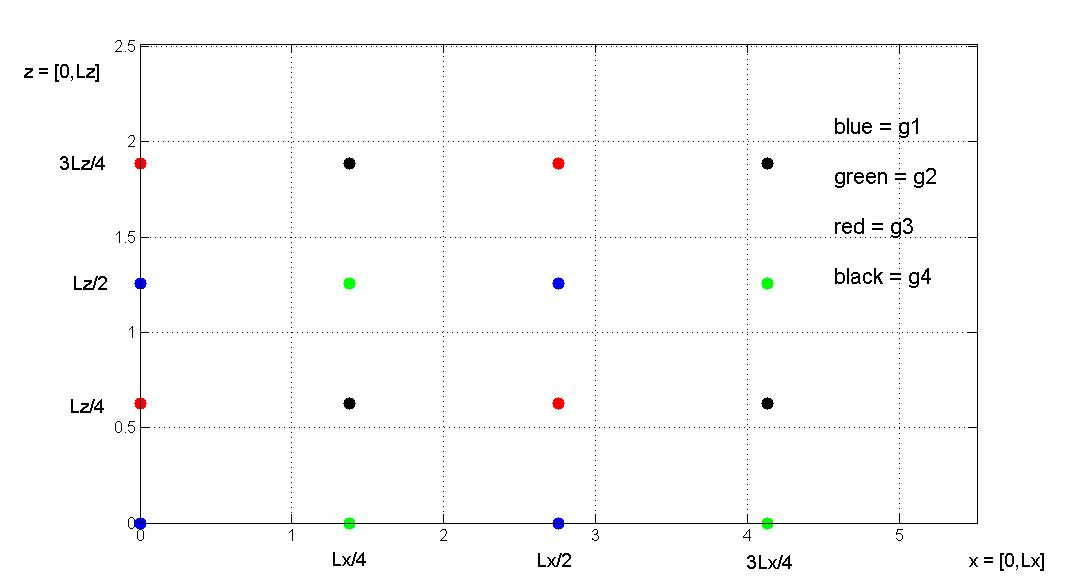
\includegraphics[width=1.0\textwidth]{stags7_26.jpg}
  \caption{
   Sets of possible \stagp s. If one of the $g$ symmetries is
   possessed, the velocity field will have \stagp s of the color
   corresponding to that symmetry.
   }
  \label{eltonFig:stags7_26}
 \end{figure}



\begin{large}
\noindent \textbf{Proof that any new \stagp\ must have a partner, symmetric about one of the previously known stagnation points} \\
\end{large}


Though our symmetry arguments do not determine whether or not there may exist \textit{additional} stagnation points which are not forced by the $g$ symmetries in the preceding section, we can in fact that show that for equilibria which exist in one of the flow-invariant subspaces that contains a $g$-symmetry (for example, $S$ has $g_3$ symmetry and $S_8$ has both $g_2$ and $g_3$ symmetry), any additional nontrivial stagnation points that exist must occur in symmetric pairs centered around the other known stagnation points.

Consider one of the equilibria in the $S$-invariant subspace, such as EQ2. Again, the
 action of $s3 \in S$ on velocity fields gives:
 \beq    s_3 \, [u, v, w](x,y,z) = [-u,-v,-w](-x,\, -y,\, -z+L_z/2)\nnu\, .
 \eeq
 If $(x_{_{SP}},y_{_{SP}},z_{_{SP}})$ is a \stagp, $[u, v,
 w](x_{_{SP}},y_{_{SP}},z_{_{SP}}) = [0,0,0]$, then
 \begin{align} s_3 \, [u, v, w](x_{_{SP}},y_{_{SP}},z_{_{SP}}) &= [-u,-v,-w](-x_{_{SP}},\, -y_{_{SP}},\, -z_{_{SP}}+L_z/2) \nnu\, \\
 &= [0,0,0](-x_{_{SP}},\, -y_{_{SP}},\, -z_{_{SP}}+L_z/2) .
 \end{align}
 Thus $(-x_{_{SP}},\, -y_{_{SP}},\, -z_{_{SP}}+L_z/2)$ is also a \stagp.


 \noindent We may parameterize a line passing through two points $(x_{1}, y_{1}, z_{1}),(x_{2}, y_{2}, z_{2})$
 as
 \begin{align}
  x &= x_{1} + (x_{2} - x_{1})t \\
  y &= y_{1} + (y_{2} - y_{1})t \\
  z &= z_{1} + (z_{2} - z_{1})t \\
  t &\in (-\infty,\infty)
 \end{align}
 
 Using the two stagnation points $(x_{_{SP}},y_{_{SP}},z_{_{SP}})$ and $(-x_{_{SP}},-y_{_{SP}},-z_{_{SP}} + L_z/2)$ this becomes
 
 \begin{align}
  x &= x_{_{SP}}(1-2t) \\
  y &= y_{_{SP}}(1-2t) \\
  z &= z_{_{SP}}(1-2t) + \frac{L_{z}}{2} t
 \end{align}
 When $t = 1/2$ this system returns $(x,y,z) = (0,0,L_{z}/4)$, showing
 that $SP_3$ lies on the line between these two \stagp s, halfway
 in between them.

 If we invoke the box periodicities: $x = x + L_{x}$, $z = z +
 L_{z}$, it is easy to show that this pair of stagnation points is also symmetric
 about any of $SP_1$-$SP_4$. For example, \\

 \noindent$\mathbf{x = x + L_{x}}$:

 \noindent $(x_{_{SP}},y_{_{SP}},z_{_{SP}})$ is a \stagp\ $\Rightarrow$
 $(-x_{_{SP}}+L_{x},-y_{_{SP}},z_{_{SP}}+L_{z}/2)$ a \stagp.
 \begin{align}
  x &= x_{_{SP}}(1-2t) + L_{x}t \\
  y &= y_{_{SP}}(1-2t) \\
  z &= z_{_{SP}}(1-2t) + \frac{L_{z}}{2} t
 \end{align}
 When $t = 1/2$ this returns $(x,y,z) = (L_{x}/2,0,L_{z}/4)$, so that the new stagnation
 points lie symmetrically on a line passing through $SP_1$. 

 For an equilibrium invariant under $S_8$, such as EQ8, existence of any additional nontrivial stagnation point will then imply \textit{two} additional stagnation points, based on the action of $g_2$ and $g_3$.
 If $(x_{_{SP}},y_{_{SP}},z_{_{SP}})$ is a \stagp, then  $(-x_{_{SP}},\, -y_{_{SP}},\, -z_{_{SP}}+L_z/2)$ and $(-x_{_{SP}} + L_x/2,\, -y_{_{SP}},\, -z_{_{SP}})$ are also \stagp s. 

 We will investigate numerical methods to determine existence of any such nontrivial stagnation points, in fact for EQ2, as we show in the next section, we do find such a point and it's symmetric partner. These additional stagnation points are critical for understanding the flow dynamics in the equilibrium field, as the stable and unstable manifolds provide us with a skeleton of the overall dynamics.
 

 
 



\section{Lagrangian Dynamics}
\label{sec:Lagrangian}


\subsection{Approach}
\label{sec:approach}

We know of the existence of  \stagp s in the flow of an equilibrium velocity field
predicted from the symmetries of \pCf. Thus the starting point for our investigation is clear; treating an equilibrium velocity field as an autonomous dynamical system we have already identified the "fixed points" of the system, which we refer to in this context as the \stagp s.  Starting a small
sphere of initial conditions around the \stagp s and evolving them
forward and backward in time gives a good estimate of what the stable and
unstable manifolds should look like. 

Using the sum formula for computing velocities at
any point in the \pCf\ domain \refeq{eqn:spectralsum}, by differentiating this formula it is a simple
matter to compute the $[3\!\times\! 3]$ {\velgradmat}
at any point. Eigenvalues and eigenvectors of this matrix will
provide linear stability analysis results and allow for more accurate computation of the stable
and unstable manifolds by starting our initial points along the directions of the eigenvectors. 


 In order to investigate additional places in the domain for which no movement occurs, we may numerically compute $|\bu|^{2}$ along a fine
grid and try to ascertain regions where it's value falls below a given threshold. Then
using interpolation in these regions, any additional  \stagp s can be
pinned down. 

Potential applications that could follow from having an understanding of the Lagrangian dynamics would range from being able to compute mixing
and diffusion properties, Lyapunov exponents, material stretching,
striation thickness, time to mix etc... Similar investigations tend to be in two dimensional closed systems (refs), but if we find we
have good Lagrangian chaos, this could provide a tangible 3D system for such investigations.






\subsection{A colorful portrait of the Upper Branch equilibrium}
\label{sec:eq2}


Our analysis is carried out for the Nagata/Walleffe
"Upper Branch" \eqv\ velocity field, EQ2, at $\Reynolds = 400$.
The cell size parameters are \beq   [L_x,2,L_z]
         = \; [2\pi/1.14,2,4\pi/5]
         ~ [5.512,2,2.513].
\label{cellW03}
\eeq

To begin, we look at the evolution of Lagrangian tracers starting on a grid of points, shown in \reffig{eltonFig:UBs}. The grid
is chosen to lie in the $[y,z]$ plane, centered at $x = L_x/2$. The initial
points are equally spaced, and offset by one position from the edge
of the box. If the number of points is chosen to be one less than a
multiple of 4, there will be points starting at $\bold{x}_{_{SP_{1}}}=(L_x/2,0,L_z/4)$ and
$\bold{x}_{_{SP_{2}}}=(L_x/2,0,3L_z/4)$. The
trajectories are integrated and run for a relatively short time. Here, the tracers are shown for $\bu$ defined as the difference from laminar flow. Just from evolving the grid of points alone we begin to get a feel for the dynamics.




EQ2 invariance under the symmetry group $S$, explained  in
\refsect{sec:symm_stag}, implies the existence of 4 \stagp s $SP_1$-$SP_4$,
\refeq{s3lagrange}.
%\bea
%  \xSP{1} &=& (L_x/2,0,L_z/4) \continue
%  \xSP{2} &=& (L_x/2,0,3L_z/4) \continue
%  \xSP{3} &=& (0,0,L_z/4) \label{s3lagrange} \\
%  \xSP{4} &=& (0,0,3L_z/4) \nnu
% \,.
%\eea
In \reffig{eltonFig:UBs}(b) the figure
from part (a) has been rotated in order
to reveal these \stagp s. The behavior of trajectories near these
fixed points reveals their  qualitative nature.
The point at $3L_z/4$ in \reffig{eltonFig:UBs}(b) appears to be an
unstable spiral, whereas the point at $L_z/4$ is probably hyperbolic. In order to verify these hypotheses, eigenvalues and
stable/unstable manifolds for these \stagp s are computed. \\


\begin{figure}[!h]
(a)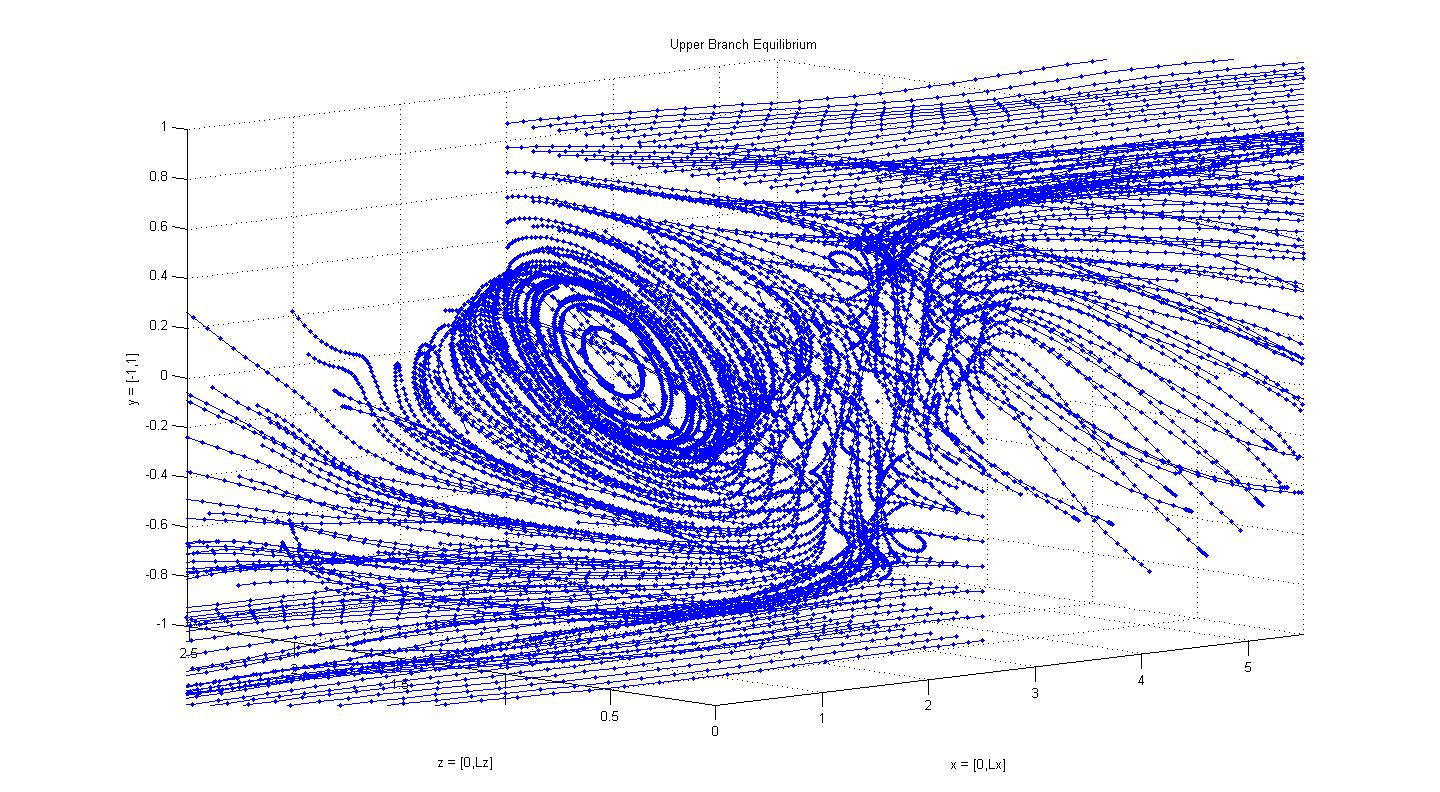
\includegraphics[width=1.0\textwidth ]{fig_UB1.jpg}
(b)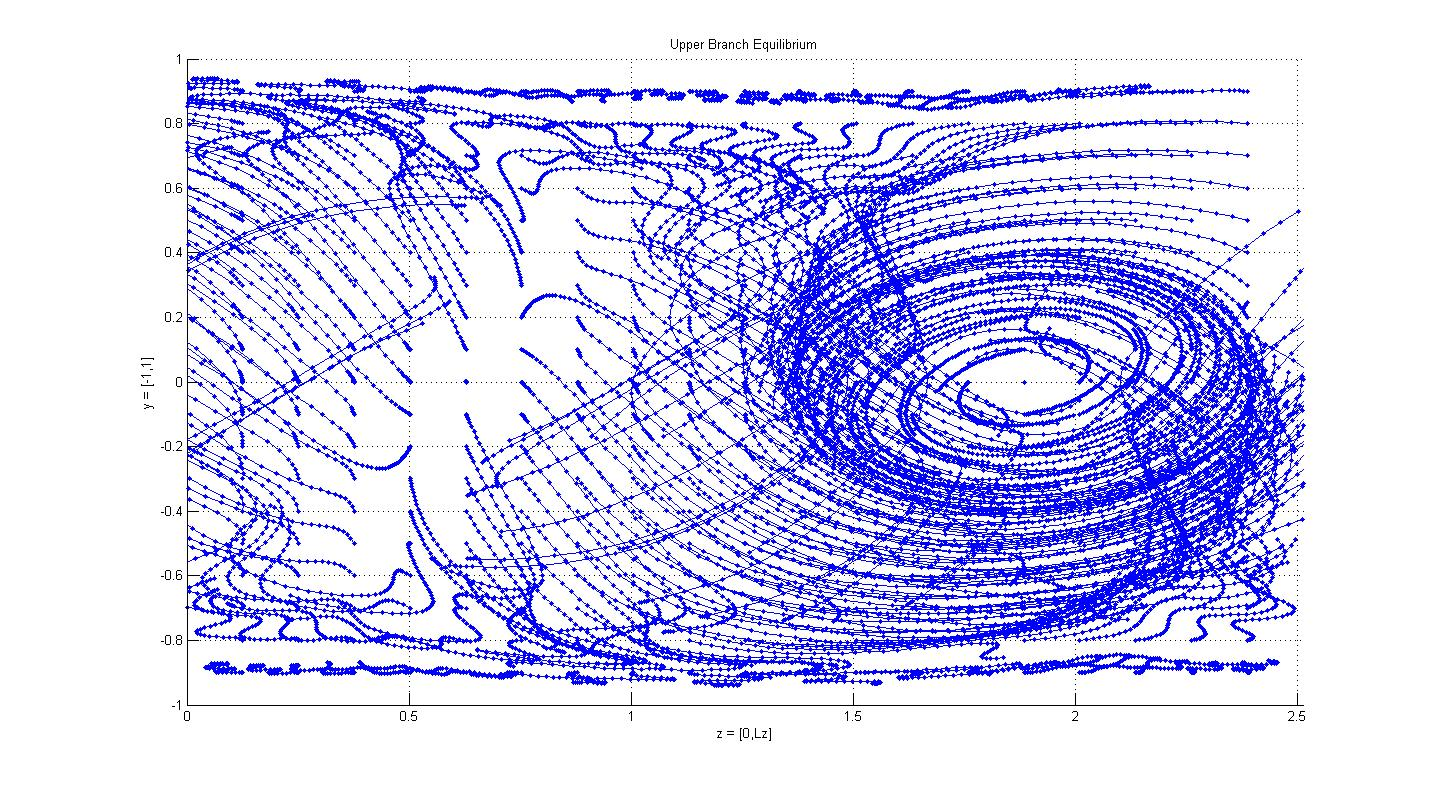
\includegraphics[width=1.0\textwidth]{fig_UB1eq.jpg}
  \caption{
  (a) {Grid of $19 \times 19$  initial points in the $[y,z]$ plane,
centered at $x = L_x/2$; integrated for 15 time units.}
    (b) { Rotated to show the 2 \stagp s}.
      }
  \label{eltonFig:UBs}
 \end{figure}

%  \begin{figure}[!h]
% (a)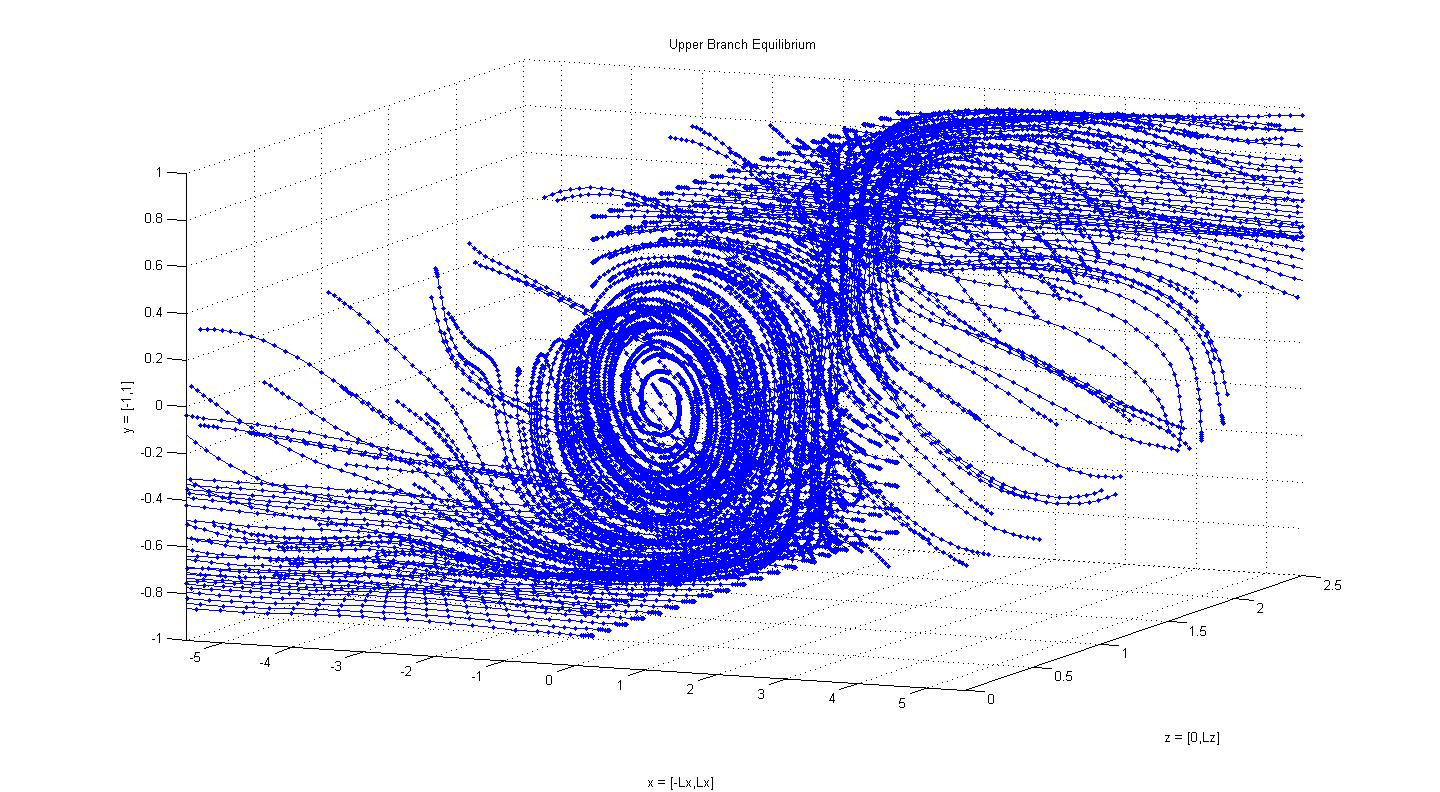
\includegraphics[width=0.8\textwidth]{fig_UB2.jpg}
% (b)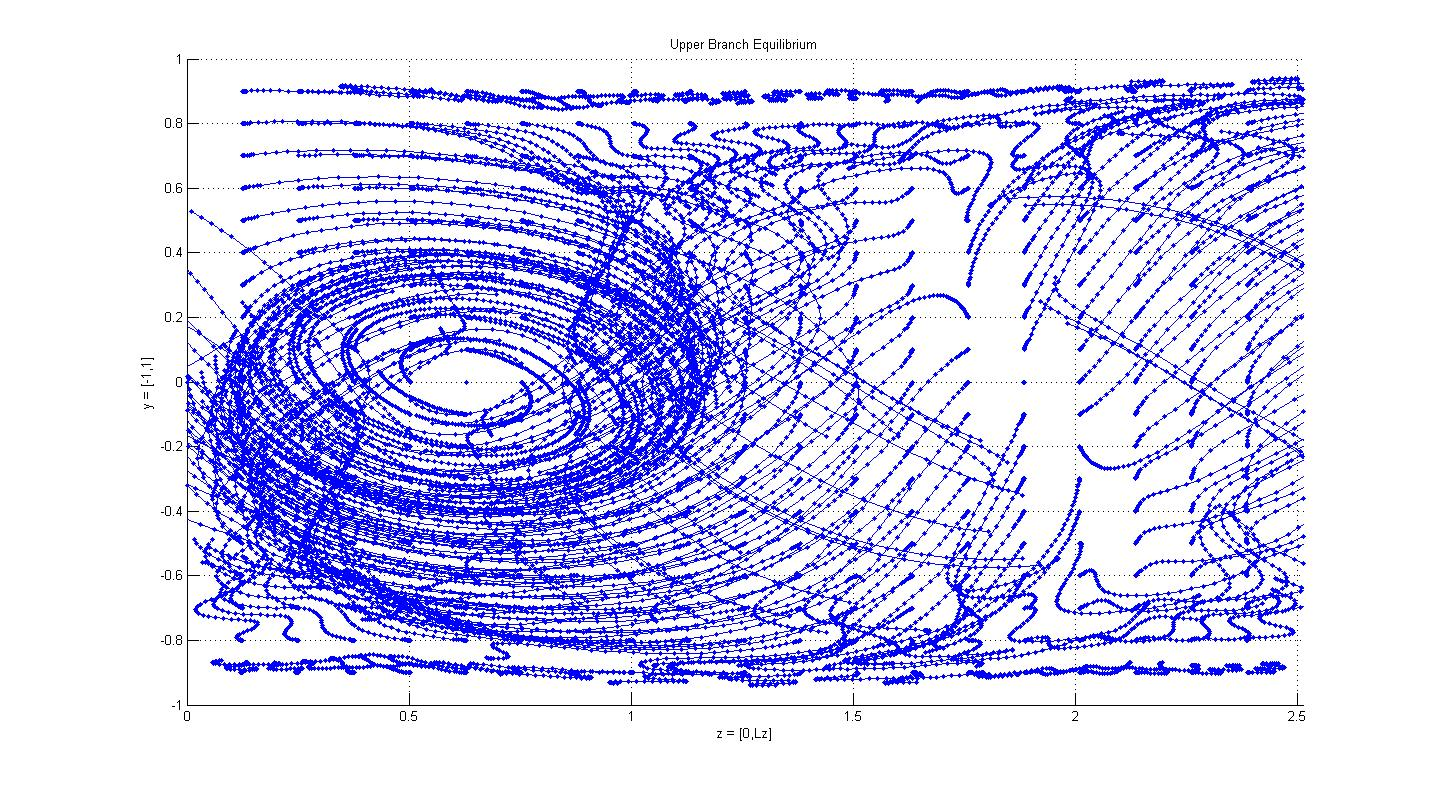
\includegraphics[width=0.8\textwidth]{fig_UB2eq.jpg}
%   \caption{
%   (a) {Grid of $19 \times 19$ initial points in the $[y,z]$ plane,
% centered at $x = 0$; integrated for 15 time units.}
%   (b) { Rotated to show the other 2 \stagp s}.
%          }
%   \label{eltonFig:UBw}
%  \end{figure}




\begin{large}
\noindent \textbf{Linearization and Stability} \\
\end{large}

For a perturbation $\delta$\bx\ away from one of the stagnation points,
the change in the velocity field is given by $\delta\bu = \Mvar
\delta\bx$ where $\Mvar$ is the nine component \velgradmat\ defined
by $\Mvar_{ij}=\frac{\partial u_{i}}{\partial x_{j}}$. Since \bu\ is
given by \refeq{eqn:spectralsum}, it is a relatively simple
extension of this formula to evaluate these partials. To find
$\partial\bu/\partial y$, one needs to use the relation
$\frac{\partial}{\partial y}T_{n}(y) = n U_{n-1}(y)$ where $T_{n}$
is the $n$th Chebyshev polynomial of the first kind and $U_{n}$ is
the $n$th Chebyshev polynomial of the second kind. Everything else
is straightforward.
The eigenvalues of $\Mvar$, evaluated at a \stagp\  give local stability
and reveal the qualitative nature of the motions nearby the \stagp.
For the \stagp s $SP_1$ - $SP_4$, the eigenvalues, eigenvectors,
and velocity gradients matrices are as follows. \\

$\bold{x}_{_{SP_{1}}}=(L_x/2,0,L_z/4)$: There are 3 real eigenvalues, two positive and one
negative.
\begin{align}
&\eigExp[1] = -0.4652099 \,,\quad
\jEigvec[1] =
\begin{pmatrix}
             {0.9844417} \cr
             {0.1743315} \cr
             {0.0219779} \cr
   \end{pmatrix} \\
    &\eigExp[2] = 0.4008961 \,,\quad \jEigvec[2] =
\begin{pmatrix}
             {0.5704000} \cr
             {-0.7666749} \cr
             {0.2947091} \cr
   \end{pmatrix} \\
    &\eigExp[3] = 0.0643139 \,,\quad \jEigvec[3] =
\begin{pmatrix}
             {0.4082166} \cr
             {0.7525949} \cr
             {0.5166819} \cr
   \end{pmatrix} \end{align}
   The \velgradmat\ is
\beq
   \Mvar =
   \begin{pmatrix}
   {-0.4305385} &  {-0.3002042} &{0.8282447} \cr
   {-0.1221356} &   {0.2456107} & {-0.1675796} \cr
   {0.0001651}  &   {-0.0828951}  & {0.1849278} \cr
            \end{pmatrix}
\eeq
    The point is a saddle; It has 1 stable dimension and a 2D plane
    of instability spanned by $\jEigvec[2]$ and $\jEigvec[3]$.
    The eigenvalues sum to 0, as is required by volume conservation.
    
     The \stagp\ $SP_4$ at
    $(0,0,3L_z/4)$ has the same eigenvalues as for $SP_1$. It's
    eigenvectors and \velgradmat\ differ by a minus sign
    in the third component (except for $\Mvar_{33}$ where the two minuses
    cancel). \\

$\bold{x}_{_{SP_{2}}}=(L_x/2,0,3L_z/4)$: There is one real, negative eigenvalue and a complex
pair with positive real part.

\begin{align}
&\eigExp[1] = -0.0352362 \,,\quad \jEigvec[1] =
\begin{pmatrix}
             {-0.9452459} \cr
             {-0.1893368} \cr
             {-0.2658228} \cr
   \end{pmatrix}
   \\
&\eigRe[2] \pm i\,\eigIm[2] = 0.0176181 \pm i\,0.0862176
   \\
&\jEigvec[2] =
\begin{pmatrix}
             {0.3737950 + 0.0544113i} \cr
             {0.2098940 - 0.4925773i} \cr
             {0.7554000} \cr
   \end{pmatrix}
\,,\quad
\jEigvec[3] =
\begin{pmatrix}
             {0.3737950 - 0.0544113i} \cr
             {0.2098940 + 0.4925773i} \cr
             {0.7554000} \cr
   \end{pmatrix}
\nnu\,.
\end{align}
The \velgradmat\ is \beq
   \Mvar =
   \begin{pmatrix}
   {-0.0316935} & {-0.0708737} &  {0.0378835} \cr
  {-0.0250579} & {-0.0218884} &  {0.0795969} \cr
   {0.0014742} & {-0.1320575} &  {0.0535818} \cr
   \end{pmatrix}
                    \eeq

    This \stagp\ spirals out in a plane given by the complex pair of
    eigenvectors. It is stable in one dimension that is dominantly
    along the $x$ direction. 
    
    $SP_3$
 at $(0,0,L_z/4)$ has the same eigenvalues as $SP_2$ and again, the
    \velgradmat\ is the same except for sign changes in
    the third component. This follows from the plane Couette symmetries. \\

\begin{large}
\noindent \textbf{Additional Stagnation Points} \\
\end{large}

Having analyzed stagnation points $SP_1$-$SP_4$, before further investigating the dynamics, it is natural to wonder whether other such stagnation points may exist that do not necessarily follow from a symmetry argument. To answer this question, as mentioned in \refsect{sec:approach}, we numerically compute $|\bu|^{2}$ along a fine
grid and look for where it's value falls below a given threshold. 

We create a more refined grid of velocities which
  is $144 \times 105 \times 144$. This is three times the 48 $\times$ 35
  $\times$ 48 grid in each dimension used to show the initial tracer trajectories, and contains about 2.2 million
  points. At each point $|\bu|^{2}$ is then calculated and at
  every point that satisfies $|\bu|^{2} < \epsilon$ for some
  arbitrarily chosen $\epsilon$, the point is plotted.

In \reffig{eltonFig:fine_usquare} we show regions in the cell where $|\bu|^{2}$ is very small for $\epsilon = 10^{-4}$, notated by the globs of blue dots. The trajectories shown, explained below, are also suggestive of the existence of a stagnation point in this region within the spiraling region. The four previously known stagnation points are identified in the figure, but we also see a couple of additional clumps. Honing in one of the suspicious clusters,
starting from the gridpoint value with smallest velocity in the suspicious region,
$\bx_{0} \approx (2.33476, 0.40952, 0.64577)$, and its reflection through
$\bold{x}_{_{SP_{1}}}$, $\bx_{0}' =2 \bold{x}_{_{SP_{1}}} - \bx_{0}$, the Newton iteration
 \beq
 \bx_{k+1} = \bx_{k} -
          {\Mvar}^{-1}(\bx_{k}) \, \bu(\bx_{k})
 \eeq
%  where $\Mvar$ is the \velgradmat.
converges rapidly to verify \textit{another} pair of \stagp s. Because we have already used notation to define points $SP_1$-$SP_8$ in \refsect{sec:symm_stag}, we refer to these new numerically discovered stagnation points as $SP_{N1}$ and $SP_{N2}$: 

\begin{align}
&\bold{x}_{_{SP_{N1}}} =(2.35105561774981,0.42293662349708,0.65200166068573)
\\
&\bold{x}_{_{SP_{N2}}}=(3.16051044117966,-0.42293662349708,0.60463540075018)
\label{eqn:newspNewt}
\,.
\end{align}
%         = [5.51156605892946182182,2,2.51327412287183459075]
We see the
 symmetry in the $y$-component of this pair, as was expected looking
 at \reffig{eltonFig:fine_usquare}.
These points are seen to be
 symmetric about the point $SP_1$
 \beq
    (\bold{x}_{_{SP_{N1}}} +\bold{x}_{_{SP_{N2}}})/2 = \bold{x}_{_{SP_{1}}}
 \,.
 \eeq

 

  \begin{center}
\begin{figure}[!h]
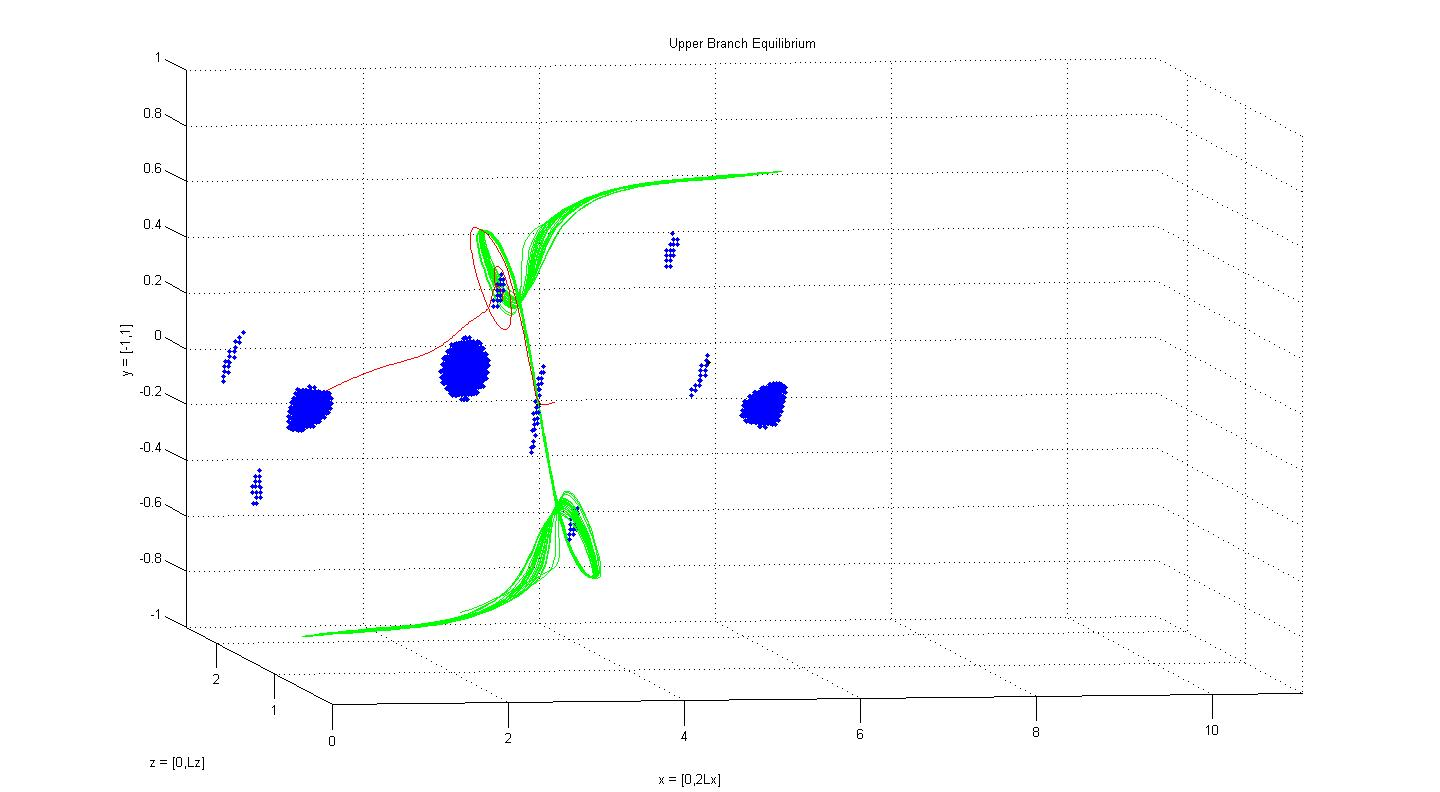
\includegraphics[width=1.0\textwidth]{fine_usquare.jpg}
  \caption{
   Blue clumps of points are where velocity squared is very close to zero.
   Shown along with the stable manifold
   of $SP_3$ (black) and the unstable manifold of $SP_1$ (green).
          }
  \label{eltonFig:fine_usquare}
 \end{figure}
\end{center}



 Repeating the linear stability analysis for $SP_{N1}$ and $SP_{N2}$: There is one real, positive eigenvalue
 and a complex pair with negative real part.

  \begin{align} &\eigExp[1] = 0.1453207 \,,\quad \jEigvec[1] =
\begin{pmatrix}
             {0.9307982} \cr
             {0.3502306} \cr
             {0.1046576} \cr
   \end{pmatrix}
   \\
&\{ \eigExp[2],\eigExp[3]\}
  = \eigRe[2] \pm i \,\eigIm[2] =  -0.0726603 \pm i\, 0.3733478
   \nnu\\
&\jEigvec[2] =
\begin{pmatrix}
             {~0.5226203} \cr
             {-0.6703938} \cr
             {~0.2065610} \cr
   \end{pmatrix}
    \,,\quad
\jEigvec[3] =
\begin{pmatrix}
             {~0.3779843} \cr
             {~
             0} \cr
             {- 0.3031510} \cr
   \end{pmatrix}
\,.
\end{align}
The \velgradmat\ is
\beq
   {\Mvar} =
   \begin{pmatrix}
   {0.0225166} &  {0.0985763} &{0.7623083} \cr
   {0.1714566} &   {-0.1275193} & {-0.6118476} \cr
   {-0.0615378}  &   {0.1755954}  & {0.1050028} \cr
            \end{pmatrix}
\,.
\eeq
We have this time a 1D unstable manifold and a 2D spiraling stable
manifold. 

 \begin{figure}[!h]
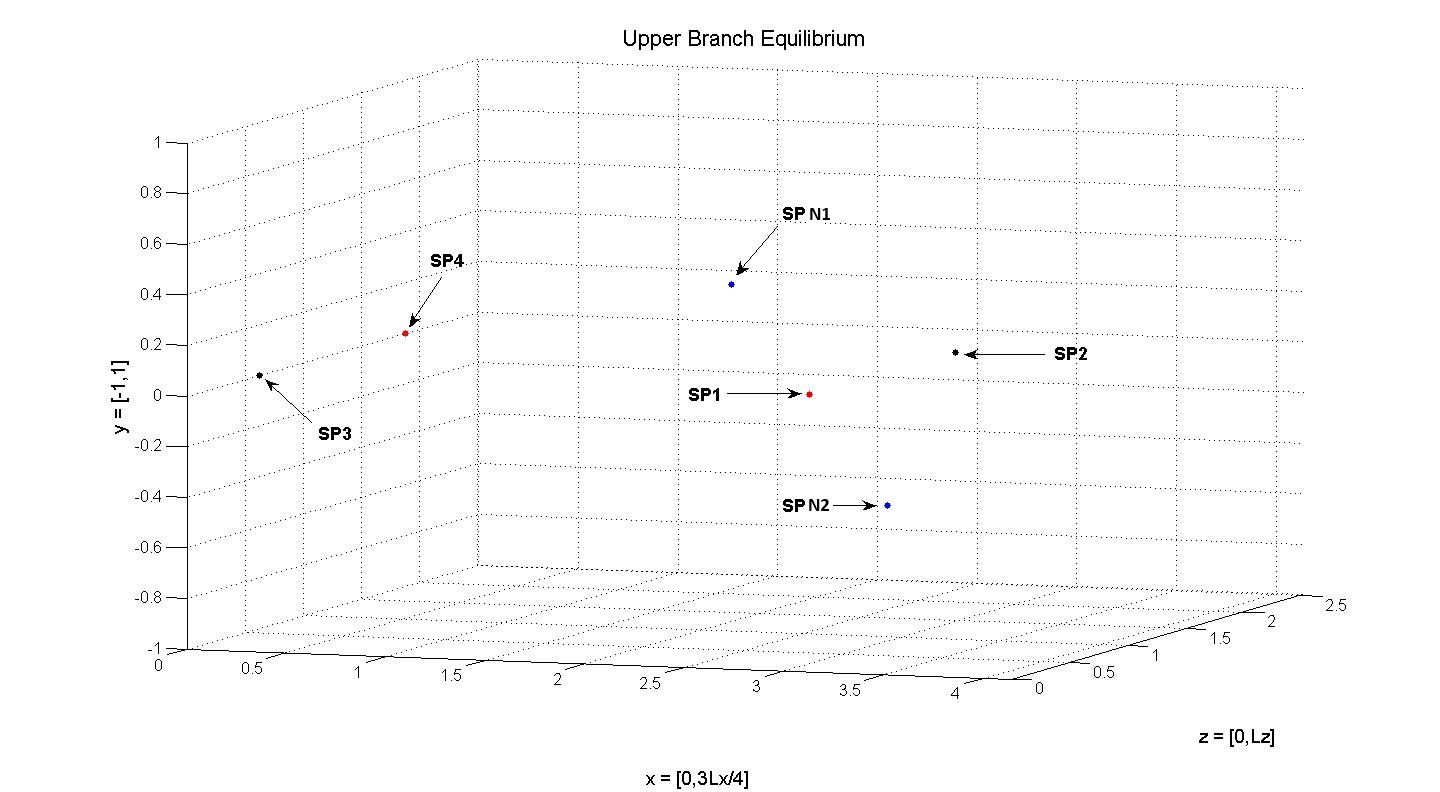
\includegraphics[width=1.0\textwidth]{stagps_edited.jpg}
  \caption{
   The 6 known unique \stagp s within one periodic box for EQ2. $SP_1$-$SP_4$ are guaranteed by EQ2 symmetries, $SP_{N1}$ and $SP_{N2}$ are determined numerically. 
   }
  \label{eltonFig:stagps_label}
 \end{figure}

 \begin{figure}[!h]
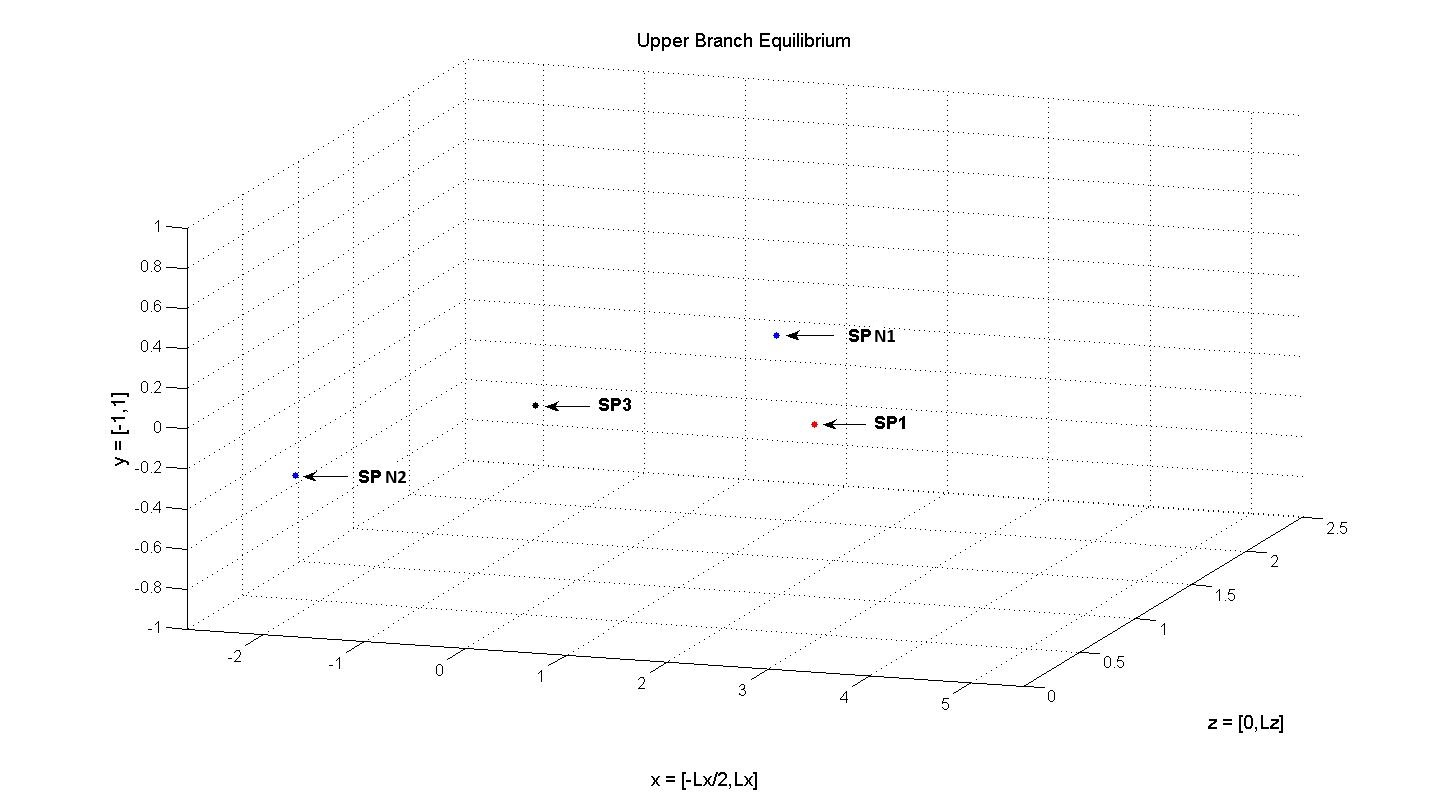
\includegraphics[width=1.0\textwidth]{stagps2_edited.jpg}
  \caption{
   The 4 \stagp s that occur within the domain $\Omega$.
   }
  \label{eltonFig:stagps_label2}
 \end{figure}

   We have been describing all \stagp s which are
   inside a single periodic cell, pictured in \reffig{eltonFig:stagps_label}. However even within this cell
   there is a redundancy in labeling all of these points as
   distinct. 
   The interesting dynamics and connections between the different \stagp s occur
 along the $x$ direction. To understand what is happening one needs
 to look only at a subset of these \stagp s that lies in the right or left half of the box, that
 is, in the interval $[0,L_{z}/2]$ or the interval $[L_{z}/2,L_{z}]$. We have chosen
 the interval $[0,L_{z}/2]$. In
 the $x$ direction the most convenient interval is not actually
 $[0,L_{x}]$, rather we look at the \stagp s in the open interval
 $(-L_{x}/2,L_{x})$, open so as to ignore the repeated translations on the boundary. Thus an alternate domain of investigation that will be conventient to sometimes use is
 \beq \Omega = (-L_{x}/2,L_{x}) \times [-1,1] \times [0,L_{z}/2].
 \eeq
 Within this domain $\Omega$ there are four \stagp s. They are $SP_1$, $SP_3$, $SP_{N1}$, and
 $SP_{N2}$, shown in
  \reffig{eltonFig:stagps_label2}. Note that $SP_{N2}$ is a
 translated version from the way it was viewed in
 \reffig{eltonFig:stagps_label}.  \\ \\
   
   

\begin{large}
\noindent \textbf{Phase portrait and heteroclinic connections} \\
\end{large}

With identification of all of the stagnation points within either the original periodic box or the cell $\Omega$, as well as the corresponding linear stability analysis, we are ready to make a complete phase space portrait for the Upper Branch, EQ2. \\

\begin{figure}[!h]
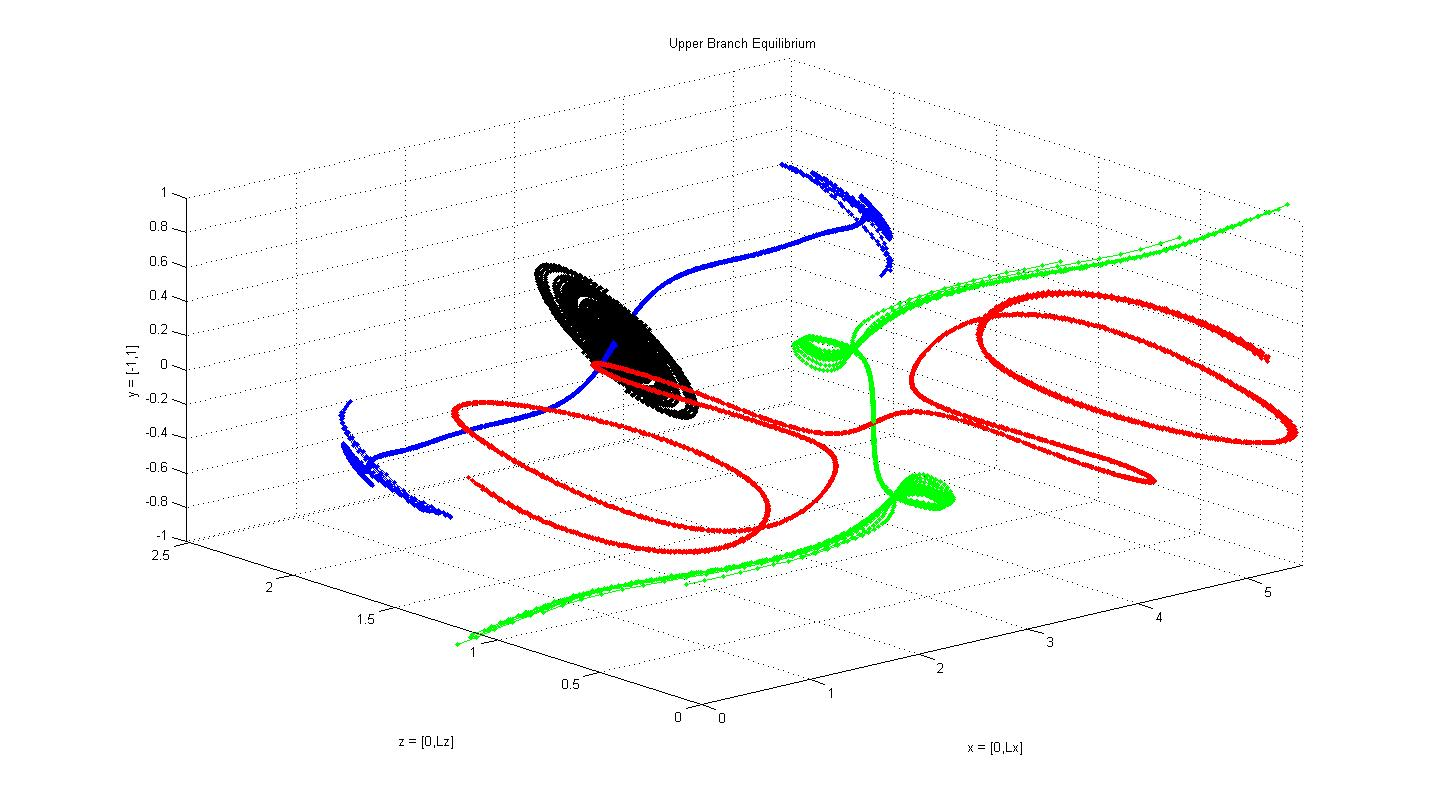
\includegraphics[width=1.1\textwidth]{manifolds_both.jpg}
  \caption{
   Segments of the stable and unstable manifolds of the \stagp s
   $\bold{x}_{_{SP_{1}}} = (L_x/2,0,L_z/4)$ and
   $\bold{x}_{_{SP_{2}}} = (L_x/2,0,3L_z/4)$. Black and green are unstable.
   }
  \label{eltonFig:manifolds_both}
 \end{figure}


    \begin{figure}[!h]
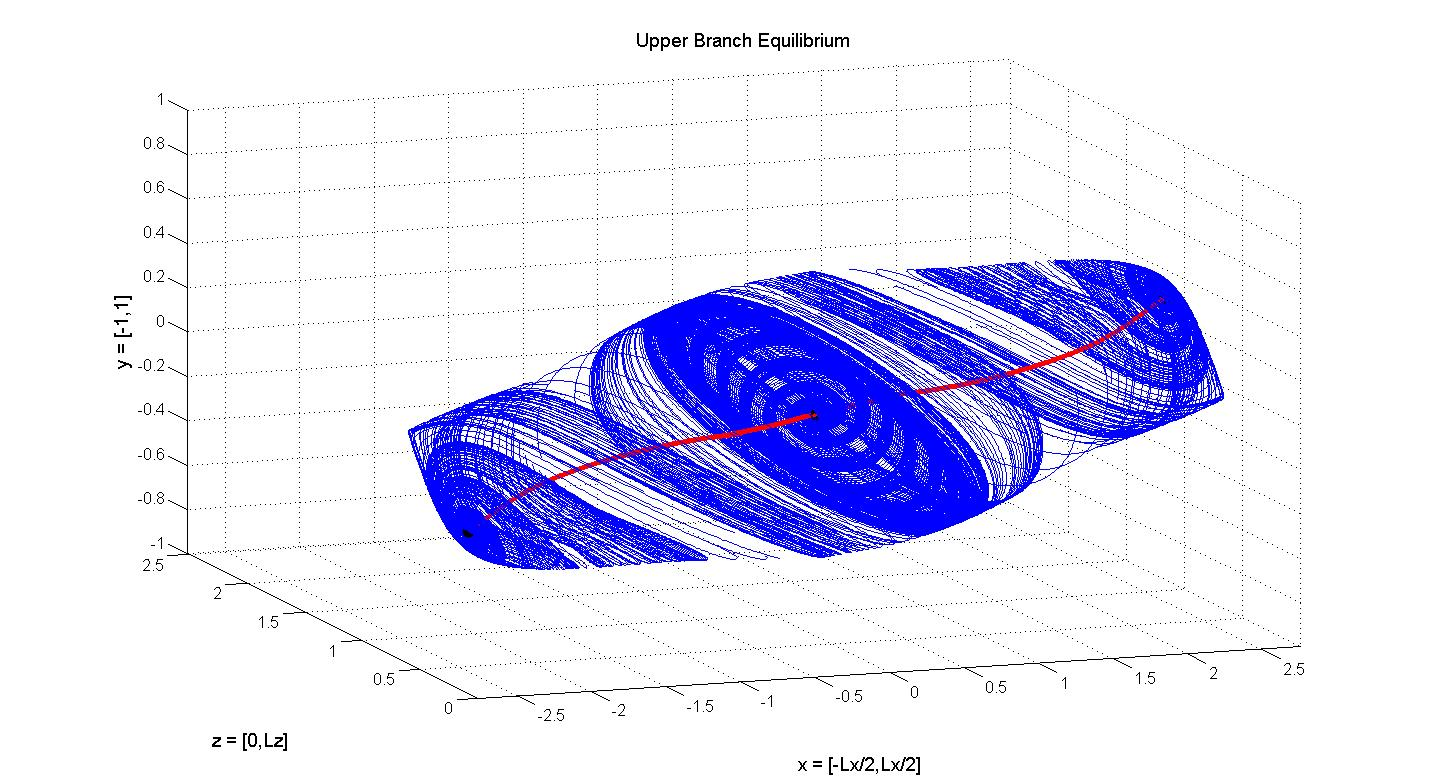
\includegraphics[width=1.1\textwidth]{man14_june3.jpg}
  \caption{
   Heteroclinic connections (red trajectories) from $SP_{N1}$ -> $SP_3$ and $SP_{N2}$ -> $SP_3$, shown in cell with $x \in$ [-Lx/2, Lx/2] along with the unstable manifold of $SP_3$.
   }
  \label{eltonFig:hetero1}
 \end{figure}




  \begin{figure}[!h]
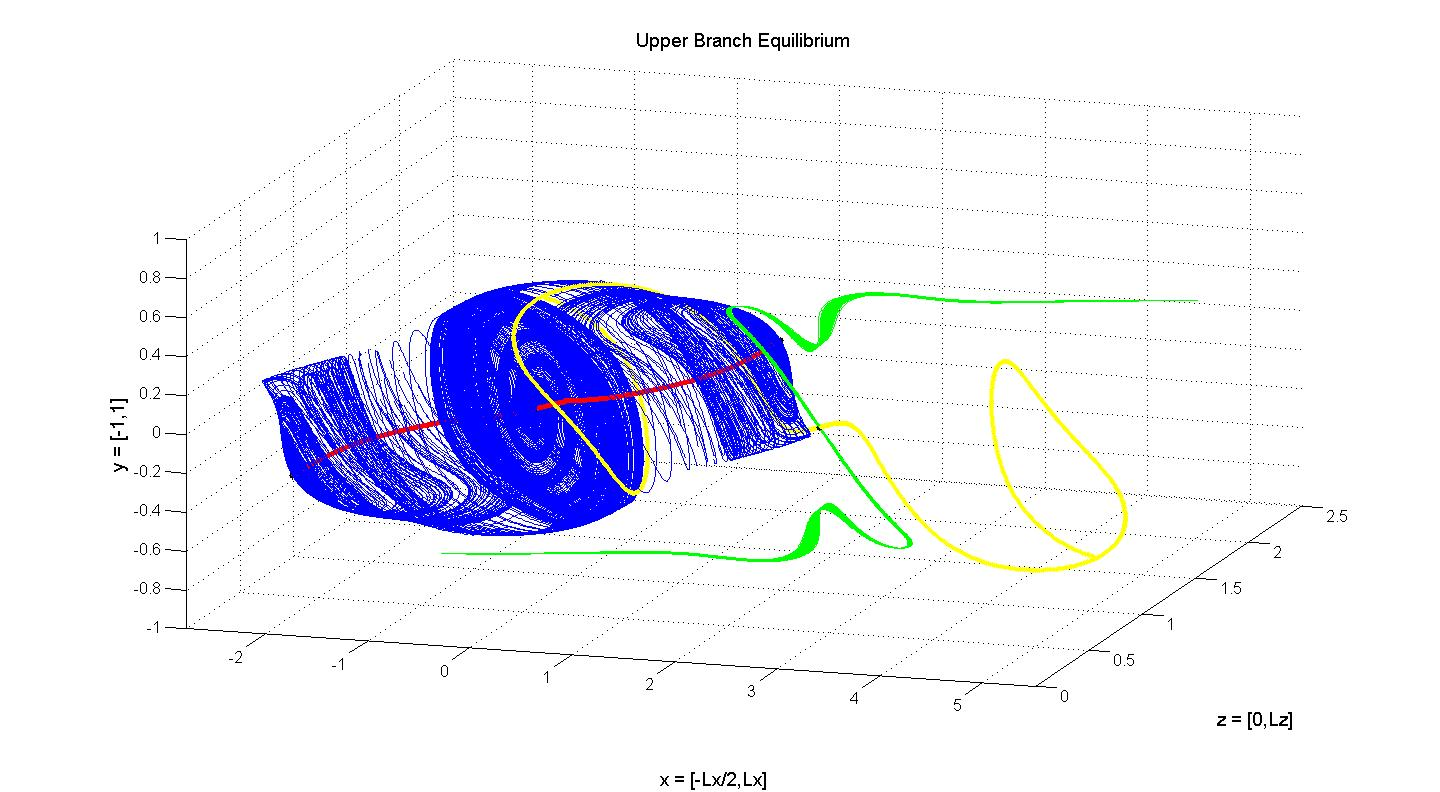
\includegraphics[width=1.1\textwidth]{june4_fig7.jpg}
  \caption{
   Portrait of the fundamental dynamics of the \stagp s $SP_1$, $SP_3$, $SP_{N1}$, $SP_{N2}$ within cell $\Omega$.
   }
  \label{eltonFig:hetero2}
 \end{figure}


 


The dynamics between the \stagp s and their translations is
   quite interesting. In \reffig{eltonFig:manifolds_both} we see a partial view of the stable and unstable manifolds of two of the stagnation points, $SP_1$ and $SP_2$, in the original periodic domain, found by integrating trajectories near the fixed points forwards and backwards in time along the stable or unstable eigenvectors. Local stability analysis shows that $SP_1$ has all real eigenvalues
with a 1D stable manifold,
and a 2D unstable manifold which is locally a plane. $SP_3$
 has a 2D unstable manifold with complex eigenvalues which spiral
 out in a plane and a 1D stable manifold. 
 
 As alluded to in \reffig{eltonFig:fine_usquare}, $SP_{N1}$ and $SP_{N2}$ sit near the center of the swirl of green coming from the unstable direction of $SP_1$. To better understand what is happening here, referring to \reffig{eltonFig:hetero1}, we compute the  stable and unstable manifolds of $SP_{N1}$ and $SP_{N2}$, where we use the shifted translation of $SP_{N2}$, along with the stable and unstable manifolds of $SP_3$. The blue surface is formed by the overlap of trajectories starting along the unstable manifold of $SP_3$ and the stable manifolds of $SP_{N1}$ and $SP_{N2}$.  We see that the stable manifold of $SP_3$ (shown by the red curves) corresponds with the unstable manifolds of $SP_{N1}$ and $SP_{N2}$, thus we have \textit{heteroclinic connections} from $SP_{N1}$ --> $SP_3$ and $SP_{N2}$ --> $SP_3$!
 The thick appearance of the red curves
 is simply so that they can be seen within the blue surface. They are actually just a single trajectory.
 
 Next we bring $SP_1$ into the picture to see the full dynamical portrait within $\Omega$. $SP_1$ has a 2D unstable manifold
 and a 1D stable manifold. The result of all of these manifolds
 plotted together is \reffig{eltonFig:hetero2}. Compare to \reffig{eltonFig:stagps_label2} to see the locations of the stagnation points. The relation of the
 stable manifold of $SP_1$ (yellow curve) and the trajectories that are driven away from $SP_1$ in the unstable direction (green)
 to those of the blue surface is quite interesting. These trajectories
 tightly hug the blue surface as they spiral around it, appearing to be shielded from entering the volume it encompasses. This could have significant implications for the consideration of fluid mixing within plane Couette flow, perhaps showing that it is difficult to achieve a uniformly mixed space for this particular equilibrium; a blob of ink that starts outside of the blue surface may have a difficult time ever entering the region!
 
 One merely translates the image in \reffig{eltonFig:hetero2} in the
 $x$ direction by an amount $L_{x}$ to give a complete picture in
 any periodic cell. The same picture will also occur symmetrically
 (translated by $L_{x}/2$ and $L_{z}/2$) in the left half of the
 box.
  
 





   \subsection{Equilibrium \tEQeight: Additional Symmetries}
   \label{sect:EQ8}

   Having thoroughly analyzed the dynamics of the "Upper Branch" Equilibrium EQ2, we next look at another equilibrium velocity field of \pCf\, EQ8. As of the time of this research, a total of 11 known equilibria have been found. EQ2 was one of the first known, dating back to 1990. And numerically it was found that EQ2 possesed the S group symmetry. Equilibrium EQ8 was found... We consider a more turbulent flow with \Reynolds\ 270. \\


\begin{large}
\noindent \textbf{Tracer dynamics and analysis} \\
\end{large}

 We start once again with a cleverly chosen grid of initial
 trajectories to get a feel for the significant structures in the
 flow. The grid is
 in a plane at $x = L_{x}/2$. The result, after a short integration
 time, is shown in \reffig{eltonFig:EQ8_grid1}. This perspective
 view already shows us quite a bit of information. Once again we
 have symmetries abound, and we know there will be at least 8 stagnation points $SP_1$-$SP_8$.  Another interesting feature of this
 plot is the four vortical structures on the left half. One final noteworthy point
  from the figure is the appearance of a perfect line segment connecting two of the
 stagnation points, which happen to be $SP_1$ and $SP_2$. 
  This strongly suggests a heteroclinic
 connection between these two \stagp s. To confirm this we
 compute the eigenvalues and eigenvectors of the \velgradmat. For
 $SP_1$, there is
 indeed a real, unstable eigenvector pointing along (0,0,1) and for
 $SP_2$ there is a real, stable eigenvector pointing along (0,0,1).
 This, together with the plot, numerically confirms the existence of the heteroclinic trajectory. The same result  holds for the shifted pair at $x = 0$. The rest of the eigenvalues/eigenvectors are given
 below. It is curious that for \tEQeight\ there is a heteroclinic connection which is a simple
 horizontal line connecting the pair of trivial \stagp s in the
 \textit{spanwise} direction, whereas for \tUB\ the connection was some
 arbitrary-looking curve in the \textit{streamwise} direction connected to a nontrivial
 \stagp. Factorization of \tEQeight\
$SP_1$ and $SP_2$ stability eigenspaces is presumably due to symmetry; the spanwise $z$ direction is a $1D$ flow-invariant subspace at
the \stagp s. That ensures the simplicity of the \hec.

\tEQeight, $SP_1$: There are two real, positive eigenvalues
 and one real, negative eigenvalue.
\bea
\left(
    \eigExp[1],\eigExp[2],\eigExp[3]
\right) &=&
      (0.363557,0.227831,-0.591389)
\label{E8SP1} \\
\left(
    \jEigvec[1],\jEigvec[2],\jEigvec[3]
\right) &=&
\left(
    \begin{pmatrix}
             {0} \cr
             {0} \cr
             {1}
    \end{pmatrix} \,,
    \begin{pmatrix}
             {-0.733415} \cr
             {-0.679780} \cr
             {0}
    \end{pmatrix} \,,
    \begin{pmatrix}
             {0.991005} \cr
             {0.133824} \cr
             {0}
    \end{pmatrix}
\right) \,.
\nnu
\eea

\tEQeight, $SP_2$: There are two real, positive eigenvalues
 and one real, negative eigenvalue.
\bea
\left(
    \eigExp[1],\eigExp[2],\eigExp[3]
\right) &=&
      (0.992857,0.255973,-1.248830)
\label{E8SP2} \\
\left(
    \jEigvec[1],\jEigvec[2],\jEigvec[3]
\right) &=&
\left(
    \begin{pmatrix}
             {~0.116961} \cr
             {-0.993136} \cr
             {0}
    \end{pmatrix} \,,
    \begin{pmatrix}
             {0.957795} \cr
             {0.287450} \cr
             {0}
    \end{pmatrix} \,,
    \begin{pmatrix}
             {0} \cr
             {0} \cr
             {1}
    \end{pmatrix}
\right) \,. \\
\nnu
\eea


   \begin{figure}[!h]
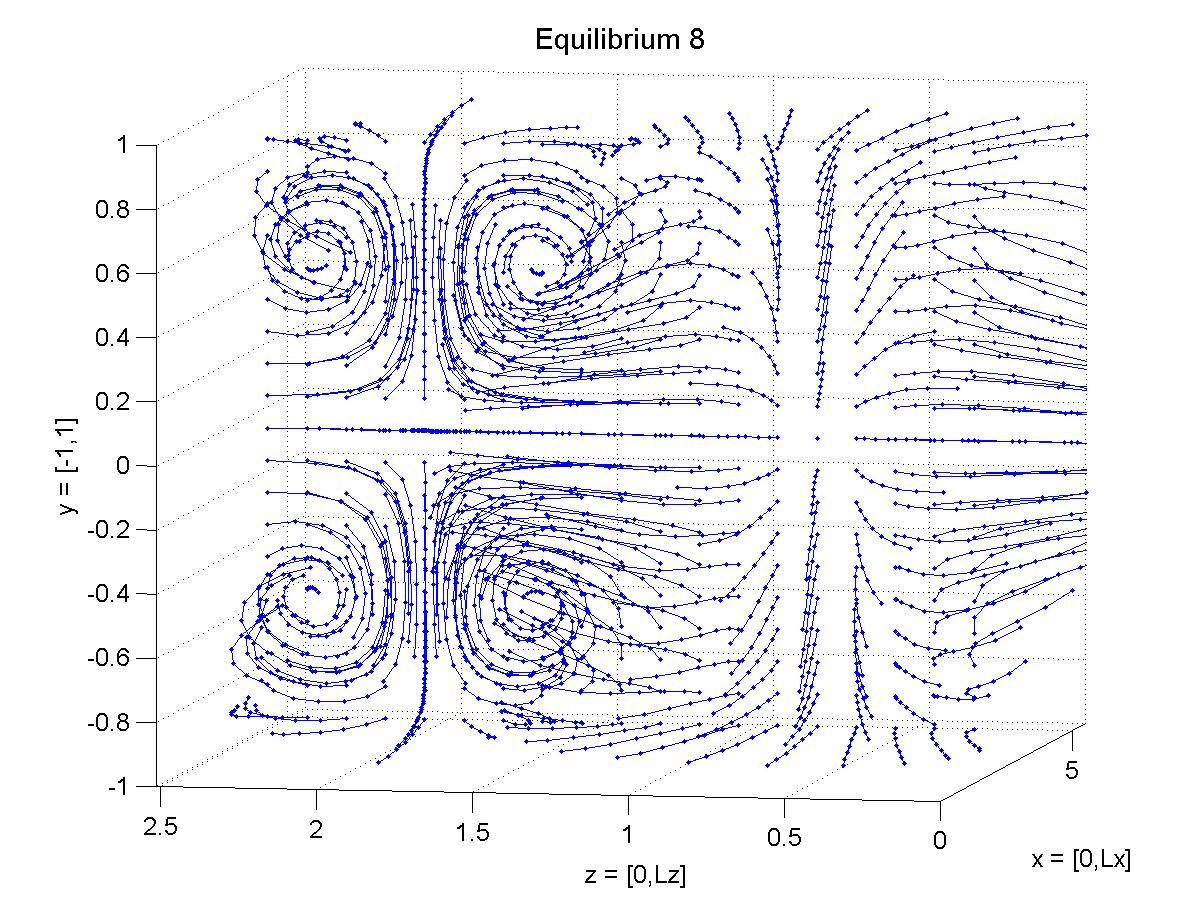
\includegraphics[width=1.0\textwidth]{EQ8_grid1.jpg}
  \caption{
   A grid of initial trajectories in the plane $x = L_{x}/2$ for EQ8,
   integrated for short time.
   }
  \label{eltonFig:EQ8_grid1}
 \end{figure}



\begin{large}
\noindent \textbf{More symmetries --> More stagnation} \\
\end{large}

Equilibrium EQ8 (as well as EQ7, not discussed here), possesses additional symmetries compared to EQ2. EQ2 is in the $S$-invariant subspace of velocity fields and EQ8 is in $S_8$ (\refsect{PCF_symm} and \refsect{sec:symm_stag}).


From \refeq{second_condition} and \refeq{s3lagrange} we know that we will have the additional stagnation points

 \bea
  \bold{x}_{_{SP_{5}}} &=& (L_x/4,0,0) \continue
  \bold{x}_{_{SP_{6}}} &=& (3L_x/4,0,0) \continue
  \bold{x}_{_{SP_{7}}} &=& (L_x/4,0,L_z/2)  \\
  \bold{x}_{_{SP_{8}}} &=& (3L_x/4,0,L_z/2) \nnu
 \,.
\eea
 Interestingly these were actually discovered numerically before the symmetry arguments were understood. A Newton search on
\tEQeight\ revealed that $(L_x/4,0,L_z/2)$ and $(3L_x/4,0,L_z/2)$
are \stagp s. From this one may deduce that symmetry $s_5$ must
hold, and it can then be checked that at any position the velocity
field is indeed invariant under $s_4$ and $s_5$. 

Stability analysis of the new set for \tEQeight\ gives the
following.

 $SP_5$: There is one real, positive eigenvalue
 and a complex pair with negative real part.
  \begin{align} &\eigExp[1] = 0.03109 \,,\quad \jEigvec[1] =
\begin{pmatrix}
             {0.85275} \cr
             {0.41774} \cr
             {-0.31355} \cr
   \end{pmatrix}
   \\
&\{ \eigExp[2],\eigExp[3]\}
  = \eigRe[2] \pm i \,\eigIm[2] =  -0.01555 \pm i\, 0.59385
   \label{EQSP5eigs}\\
&\jEigvec[2] =
\begin{pmatrix}
             {~0.24762} \cr
             {-0.31442} \cr
             {~0.69906} \cr
   \end{pmatrix}
    \,,\quad
\jEigvec[3] =
\begin{pmatrix}
             {-0.20793} \cr
             {~0.55489} \cr
             {~0} \cr
   \end{pmatrix}
\,.
\end{align}
 We have a 1D unstable manifold and a 2D in-spiral
stable manifold. All four of the new points have the same
eigenvalues. $SP_5$ and $SP_8$ have the same eigenvectors, as do $SP_6$
and $SP_7$ whose eigenvectors differ from $SP_5$ only by the sign of
the third component for \jEigvec[1] and by the sign of the first and
second components for \jEigvec[2] and \jEigvec[3].

As another consequence of
numerically searching for \stagp s, the figures produced by
plotting gridpoints where velocity is small, using a cutoff
value of $|\mathbf{u}|^{2}$ which is too large to be useful for
finding \stagp s, we instead find a plot showing
intricate patterns in the flow. \reffig{eltonFig:usquare_EQ8_1} shows a 3D
perspective view of these points, and
\reffig{eltonFig:usquare_EQ8_2} 
shows the projection of \reffig{eltonFig:usquare_EQ8_1} onto the $xz$ plane. These plots may indicate the existence of invariant tori and quasiperiodic dynamical behavior. \\

\begin{figure}[!h]
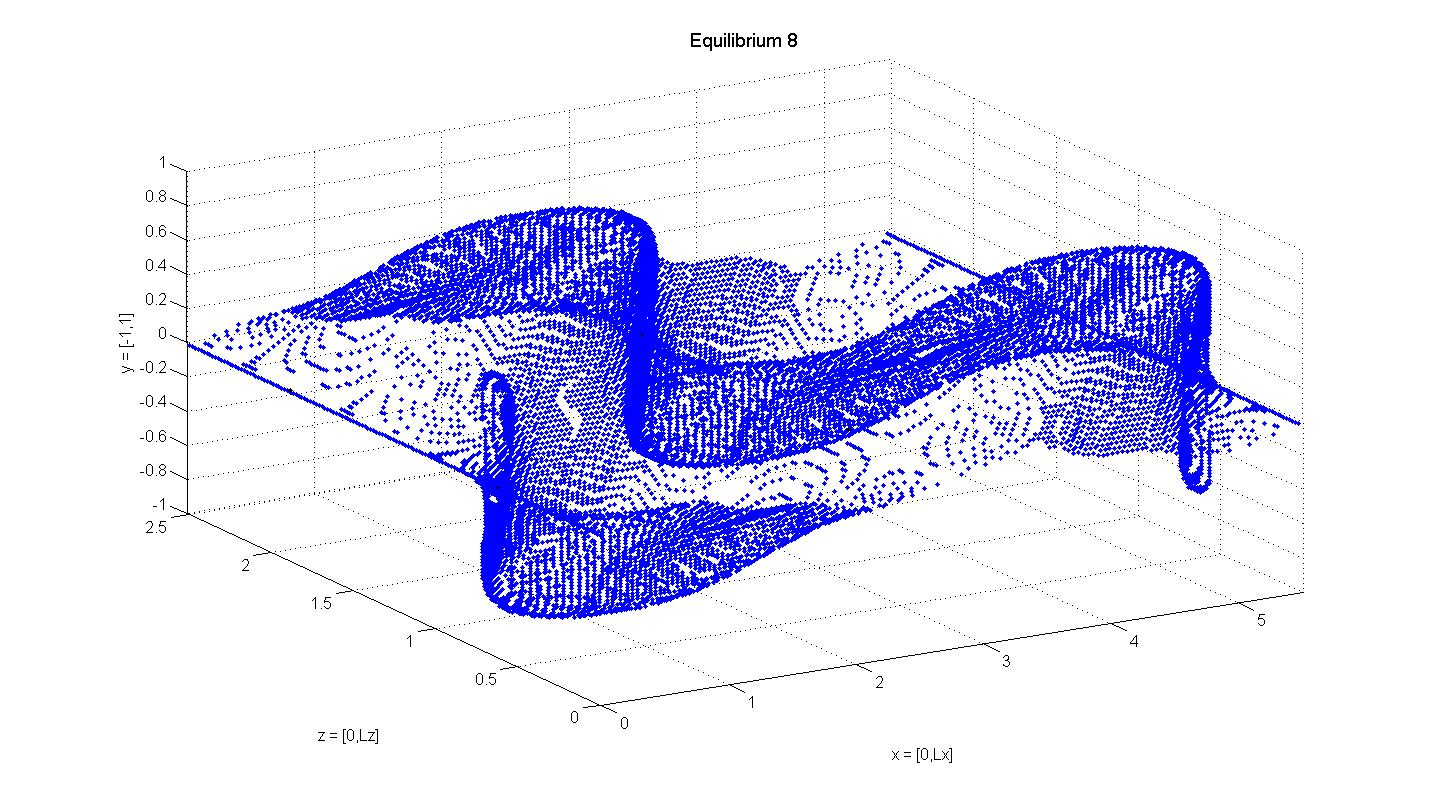
\includegraphics[width=1.0\textwidth]{usquare_EQ8_cute1.jpg}
  \caption{
   A plot of points whose value of velocity squared falls below an
   arbitrary cutoff of $5\times 10^{-7}$. Perspective view.
   }
  \label{eltonFig:usquare_EQ8_1}
 \end{figure}

 \begin{figure}[!h]
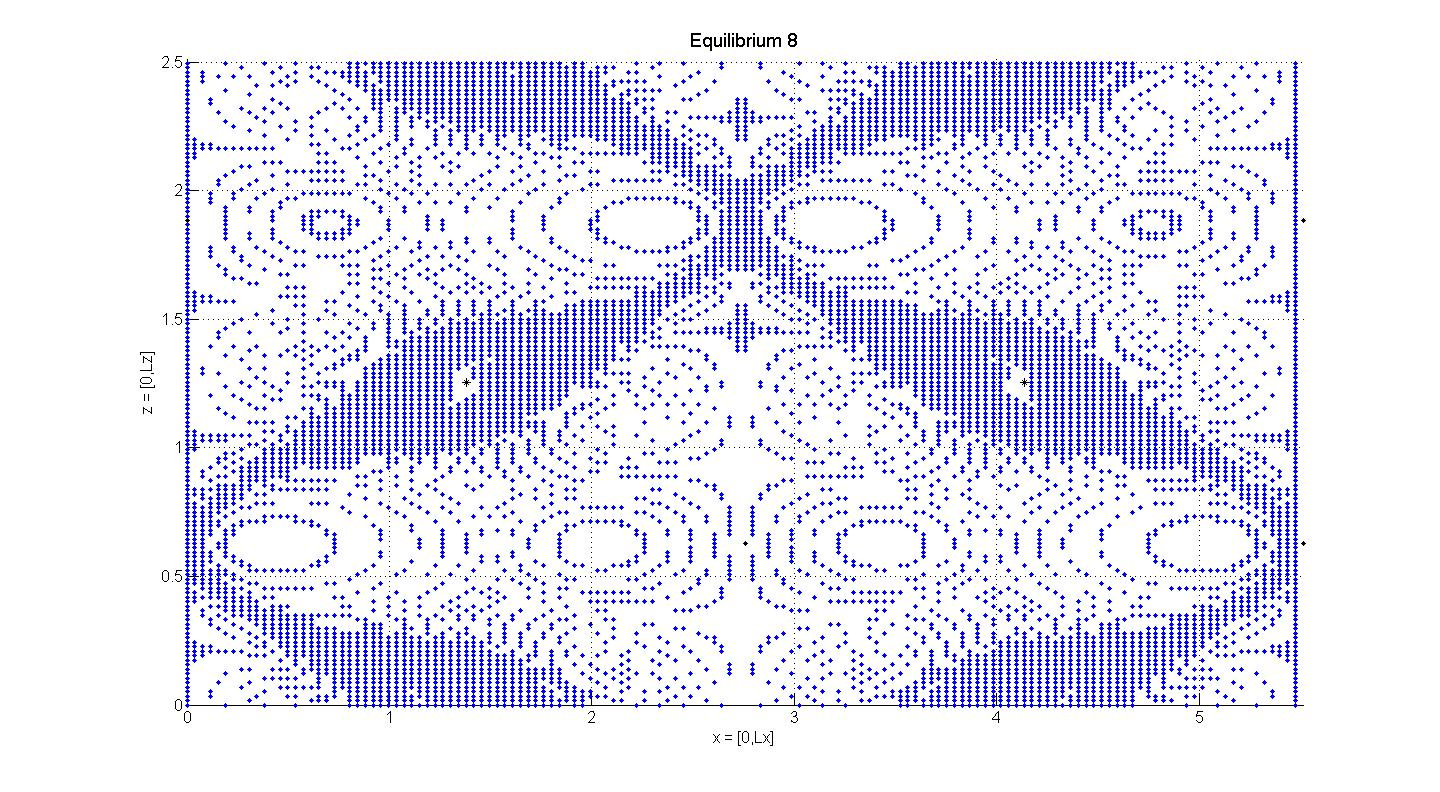
\includegraphics[width=1.0\textwidth]{usquare_EQ8_cute2.jpg}
  \caption{
   A plot of points whose value of velocity squared falls below an
   arbitrary cutoff of $5\times 10^{-7}$. Projection onto the $xz$
   plane.
   }
  \label{eltonFig:usquare_EQ8_2}
 \end{figure}




  

 







\section{Conclusion}
\label{sec:conclusion}


%%% Acknowledgements %%%
\section{Acknowledgments}
Acknowledgment. 











\section{Reading assignments}
\label{sect:Reading}


\subsection{Keywords: Lagrangian mixing in turbulence}

Do literature review for Lagrangian mixing: possible keywords
to google:
\begin{itemize}
\item
    tracer particles in turbulent ...
\item
    Lagrangian dynamics in turbulence
\item
    inertial particles
\item
    Lyapunov exponents of heavy particles in turbulent flows
\end{itemize}

Possible authors (still to check)
\begin{itemize}
\item
Krzysztof Gawedzky (Lyon)
\item
    B. Eckhardt (Marburg):
Geometry of particle paths in chaotic and turbulent flows
\item
    Jean-Francois Pinton (Lyon): Lagrangian experiments
\end{itemize}


\subsection{Articles and books of potential interest}

\medskip\noindent {\bf  PC 2015-08-09}: This indeed is very interesting,
thanks!

\medskip\noindent {\bf Mohammad 2015-08-04}: Of possible interest:
\arXiv{1508.00062} {\em Quantitative Quasiperiodicity}, by
S. Das et al. (2015).

\medskip\noindent {\bf Mohammad 2015-06-30}: Of potential interest to Predrag:
\textit{A dynamical Zeta function for group actions}, Richard Miles.
\arXiv{1506.08555}

\medskip\noindent {\bf  Jean-Luc Thiffeault 2009-3-2}:
Article with Emmanuelle Gouillart, Olivier Dauchot
 and St\'ephane Roux\rf{GDTR08},
``Open-flow mixing: Experimental evidence for strange eigenmodes''
is perhaps worth a read.

\medskip\noindent {\bf  PC 2009-1-20}:
This Master's thesis announcement,
\HREF{http://www.nbi.ku.dk/english/Calendar/Activities_09/msc_abh_23.01.09/}
     {Semi- Lagrangian Methods in Air Pollutions Models},
might have some interesting pointers to
the Lagrangian tracing and mixing literature.

\medskip\noindent {\bf  PC 2008-8-22}:
check out the talk of (and search for articles by)
\HREF{http://www.newton.ac.uk/programmes/HRT/seminars/092215003.html}
     {B. Sawford}:
  	``A Lagrangian view of scalar transport and mixing.''
(Webcast on the Newton Institute homepage.)

\noindent
\HREF{http://www.newton.ac.uk/programmes/HRT/seminars/100210301.html}
    {GL. Eyink} (Johns Hopkins)
  	``Turbulent Lagrangian dynamics of vortex and magnetic-field line''
is a smart guy, this might be worth reading/listening to.
(Webcast on the Newton Institute homepage.)

\noindent
I have not had much luck understanding
\HREF{http://www.newton.ac.uk/programmes/HRT/seminars/100209001.html}
        {L. Biferale} (Tor Vergata)
  	``Lagrangian velocity statistics in turbulence: theory, experiments and numerics,''
in the past, but one could give it a try.
(Webcast on the Newton Institute homepage.)


Ottino\rf{Botti89}
% , J.M. \underline{The kinematics of mixing: stretching, chaos,
% and transport}. Cambridge University Press, 1989.
\\

\noindent
 Chat\'e, H.; Villermaux, E.; and Chomaz, J.M.
{\em Mixing: Chaos
and Turbulence}\rf{chat_mixing99}

\noindent
    Solomon,T.H. \etal "Lagrangian chaos and multiphase processes in
    vortex flows"\rf{solLagr03}.

\noindent
 Fogleman, M.A.; Fawcett, M.J.; and Solomon, "T.H.
Lagrangian chaos and correlated Lévy flights in a non-Beltrami flow:
Transient versus
long-term transport"\rf{fogleman01}.

\noindent
 Du, Yunson and Ott, Edward.
"Growth rates for fast kinematic dynamo instabilities of chaotic
fluid flows"\rf{du_growth06}.

\noindent
 Castelian, Cathy; Mokrani, Asen; Le Guer, Yves;
Peerhossaini, Hassan. "Experimental study of chaotic advection
regime in a twisted duct flow"\rf{castel01}.


d'Ovidio \etal\rf{dovidio08}
     ``Comparison between Eulerian diagnostics and finite-size
    Lyapunov exponents''
    might be worth a quick read.

\medskip\noindent {\bf  Jean-Luc Thiffeault 2001-8-29}:
Read T\'{e}l articles\rf{KarTel97,Tel2000},
they present the basic ideas: the first\rf{KarTel97} is
unphysical and the "openness" of the flow comes from having sinks and
unbounded trajectories.  The second\rf{Tel2000} scatters tracers off a Von Karman
vortex street, where they get stuck behind the cylinder for a while in
the mixing region.

\medskip\noindent {\bf  JRE 2008-12-8}:
G. Haller. "Distinguished material surfaces and coherent structures in three dimensional fluid flows". Physica D, 149. 2001. 248.


\medskip\noindent {\bf  PC 2008-7-12}:
read
\HREF{http://arxiv.org/abs/0807.0678}
     {Dullin and Meiss}\rf{dullin-2008} on ``Quadratic
Volume-Preserving Maps.'' They study the situation when two
\stagp s are saddle-foci with intersecting two-dimensional
stable and unstable manifolds that bound a spherical
``vortex-bubble.'' Probably not seen in your case, but they
write well, and they give you many pointers to $3D$ flows literature.
If you read some of that, please enter it into elton.bib, and
write notes in your blog about what's in these articles.

\medskip\noindent {\bf  PC 2008-7-11}:
Search for, read (and explain to Predrag)
literature on $3D$ flows. There are 2 aspects that surely have much
literature:
    \begin{enumerate}
      \item
$3D$ volume conservation makes these flows
almost symplectic - in particular, Poincar\'e sections of periodic
orbits are area-preserving
      \item
Reversibility. They are presumably the same forward and
backward in time. This discrete symmetry leads to infinite families
of ``symmetry lines'' on which important sets \eqva\ and
\po s lie, and ease the searches for them, as existence of
symmetry line reduces the dimensionality of the search,
They of might be what
leads to symmetry lines discussed by JRE in \refsect{sect:stagpairs}.
However, due to the convective term in \NSe\ I have not been able to
see how reversibility works, other than for
{\velgradmat} $ {\Mvar} $,

    \end{enumerate}

\begin{description}


    \PCpost{2008-5-15}{ Read (and explain to Predrag)
this frequently cited article on $3D$ flows:
Chong, {Perry} and {Cantwell}\rf{ChPeCa90}
    }

    \PCpost{2007-11-2}{ Read (and explain to Predrag)
Schneider recommendations - Homann, Dreher and Grauer\rf{homann-2007}
and  P.K. Yeung and Pope\rf{YeuPop06}
(the P.K. is just next 10 buildings away).
    }

    \PCpost{2007-12-22}{ Read (and explain to Predrag)
Mathur, Haller, Peacock, Ruppert-Felsot, and Swinney, ``Uncovering
the Lagrangian Skeleton of Turbulence''\rf{MHPRS07}. Predrag put a
copy into
\HREF{http://ChaosBook.org/library/index.html\#HallerPRL07}
     {ChaosBook.org/library}.
     }

    \PCpost{2007-12-22}{ Read (and explain to Predrag)
Arneodo \etal\rf{ABBBBB08}, ``Universal intermittent properties of
particle trajectories
              in highly turbulent flows.''
    }


    \PCpost{2006-06-18}{
Not directly relevant to us now, but \refref{OleMog07} has exact analytic
solutions of GOY model - perhaps of interest to make connections with the
Kolmogorov obsessed.
    }

    \MMFpost{2014-10-21}{
Added two references to \texttt{elton/public\_html/papers}
for mix-norms (measures of mixing efficiency):

\emph{A multiscale measure for mixing},
George Mathew, Igor Mezi\'c and Linda Petzold (2005)

\emph{Optimal stirring strategies for passive
scalar mixing},
Zhi Lin, Jean-Luc Thiffeault
and Charles R. Doering
    }

    \PCpost{2014-11-04}{
    Thanks, will study...
Repository gets very huge very quickly if we add *.pdf's of papers to it.
We enter them into \emph{elton/bibtex/elton.bib} and put the pdf's of
papers into \texttt{ChaosBook.org/library/}. Will show you how.
    }

    \PCpost{2014-11-04}{
Noticed two papers of possible interest to Mohammad:

Ajinkya Dhanagare, Stefano Musacchio and Dario Vincenzi,
{\em Weak-strong clustering transition in renewing compressible flows}
(\arXiv{1411.0110}; J. Fluid Mech., in press):
``
  We investigate the statistical properties of Lagrangian tracers transported
by a time-correlated compressible renewing flow. We show that the preferential
sampling of the phase space performed by tracers yields significant differences
between the Lagrangian statistics and its Eulerian counterpart. In particular,
the effective compressibility experienced by tracers has a non-trivial
dependence on the time correlation of the flow. We examine the consequence of
this phenomenon on the clustering of tracers, focusing on the transition from
the weak- to the strong-clustering regime. We find that the critical
compressibility at which the transition occurs is minimum when the time
correlation of the flow is of the order of the typical eddy turnover time.
Further, we demonstrate that the clustering properties in time-correlated
compressible flows are non-universal and are strongly influenced by the
spatio-temporal structure of the velocity field.''

\emph{On the use of the theory of dynamical systems for transient problems}
by Ugo Galvanetto and Luca Magri,
(\arXiv{1411.0111};
Nonlinear Dynamics 74,  pp 373-380,
DOI: 10.1007/s11071-013-0976-7)
\\
 ... address dynamical systems
with parameters varying in time. An idea to predict their behaviour is
proposed. These systems are called \emph{transient systems}, and are
distinguished from \emph{steady systems}, in which parameters are constant. In
particular, in steady systems the excitation is either constant (e.g. nought)
or periodic with amplitude, frequency and phase angle which do not vary in
time. We apply our method to systems which are subjected to a transient
excitation, which is neither constant nor periodic. The effect of switching-off
and full-transient forces is investigated. The former can be representative of
switching-off procedures in machines; the latter can represent earthquake
vibrations, wind gusts, etc. acting on a mechanical system. This class of
transient systems can be seen as the evolution of an ordinary steady system
into another ordinary steady system, for both of which the classical theory of
dynamical systems holds. The evolution from a steady system to the other is
driven by a transient force, which is regarded as a map between the two steady
systems.''

I have not studied either, so I do not know if they are any good.
   }

    \MMFpost{2015-02-12}{
 A cute piece of math: {\it Nonlinear Dynamics of
the Rock-Paper-Scissors Game with Mutations}
Toupo and Strogatz.
Read the paper \arXiv{1502.03370}.
    }

    \PCpost{2015-02-16}{
Very cute. But that's the thing about Strogatz - writes beautifully,
but he'll never leave 2 dimensions :)
    }

    \PCpost{2015-07-20}{
Abud and Caldas\rf{AbuCal15} write in {\em On {Slater's} criterion for
the breakup of invariant curves}: ``Slater's theorem states that an
irrational translation over a circle returns to an arbitrary interval in
at most three different recurrence times expressible by the continued
fraction expansion of the related irrational number. The hypothesis
 is that Slater's theorem can be also verified in
the dynamics of invariant curves. Hence, we use Slater's theorem to
develop a qualitative and quantitative numerical approach to determine
the breakup of invariant curves in the phase space of area-preserving
maps.''
    }

    \PCpost{2015-12-04}{                                        \toCB
Weiss and Knobloch\rf{WeiKno89} write in
{\em Mass transport and mixing by modulated traveling waves}:
``
Particle transport and mixing in modulated traveling waves in a
binary-fluid mixture heated from below is studied numerically. The fluid
divides into three regions separated by Kolmogorov-Arnol'd-Moser curves:
a core region where particles are carried along with the wave (trapped),
an outer region where particles are left behind by the wave (untrapped),
and a separatrix layer between the two where particles chaotically
alternate between being trapped and untrapped. The probability
distributions for the lengths of individual trapped and untrapped events
are sharply peaked at small times, have a power-law decay, and exhibit
similar complex structure. The core and outer regions are responsible for
long-range transport with no diffusion. The chaotic separatrix layer
gives rise to long-range transport with enhanced mixing and anomalous
diffusion.
''

Gottwald and Melbourne\rf{GottMel13} make a distinction
between `strong' and `weak chaos'. They write:
``
we adopt the standard perspective of decomposing the dynamics
into the dynamics on the symmetry group and the dynamics
orthogonal to it. Systems with symmetry, or ``equivariant dynamical
systems,'' thus are cast into a so-called skew product
\[
\ssp=f(\ssp)
    \,,\qquad
\dot{\LieEl} = \LieEl \Lg(\ssp)
\]

Given a certain shape dynamics
(regular, strongly chaotic or weakly chaotic), can we say anything
about the growth rate of solutions on the group? More specifically,
what is the expected diffusive behavior?

For anisotropic systems, strong chaos leads to diffusive behavior
(Brownian motion with drift) and weak chaos leads to superdiffusive
behavior (Lévy processes with drift). For isotropic systems, the drift
term vanishes and strong chaos again leads to Brownian motion. We
establish the existence of a nonlinear Huygens principle for weakly
chaotic systems in isotropic media whereby the dynamics behaves
diffusively in even space dimension and exhibits superdiffusive behavior
in odd space dimensions.
''
    }

\end{description}







\bibliographystyle{unsrt} %prsty} %apsrev} %plain}
\bibliography{../bibtex/elton}



  \renewcommand{\ssp}{a}            %state space point
  \renewcommand\xInit{{a_0}}        %initial x
  \renewcommand{\deltaX}{{\delta a}}    %trajectory displacement
  \renewcommand\velField[1]{{F(#1)}}    %Gibson statespace velocity field
  \renewcommand\velField[1]{{u(#1)}}    %Eulerian statespace velocity field


\end{document}
